\section{Analysing Conflict}\label{conflict}
In software development, especially in agile methods, conflict analysis is an important task to ensure the coherence and functionality of the system to be developed. A conflict is defined as a inconsistency that arises when two or more requirements, often encapsulated as USs, contradict each other. This section will introduce and define conflict analysis, focusing on the concept of \textit{content inconsistency} between USs.

The main objective of this analysis is to rationalise the software development workflow by semantically identifying conflicts between the USs within the backlog of a project.

A conflict of requirements arises when two or more USs show contradictions or inconsistencies. This can manifest itself in various forms, e.g. in the manipulation of the same resource by several USs at the same time, in overlapping functions or in conflicting conditions.

\begin{example}
	Considering following USs:\\\\
	user\_story\_13: "\#G03\# As a Staff member, I want to Apply a Hold, so that I can prevent progression through the workflow or other actions in the system until the issue is resolved."\\\\
	user\_story\_14: "\#G03\# As a Staff member, I want to Remove a Hold, so that I can allow progression through the workflow or other actions in the system now that the issue has been resolved."\\\\
	In this example, user\_story\_14 deletes a resource that is used by user\_story\_13. This means that user\_story\_13 cannot be applied at all if user\_story\_14 is executed first, which leads to a conflict between these USs.
\end{example}

In section \ref{conflict_requirement}, we present the requirements and functional needs that serve as input for the design phase in order to fulfil the requirements. In section \ref{conflict_desing} we explain the design decisions of the workflow shown in figure \ref{fig:conflict_operational_flow} and explain how the architecture is structured. 

\subsection{Requirements}\label{conflict_requirement}
In order to accomplish the analysis of conflicts in USs we try to address following functional requirements:
\begin{itemize}
	
	\item As a user, I want to perform semantic analysis on user stories within a specified project backlog, so that I can identify and address conflicts effectively.
	
	\item As a user, I want a report on the US-pairs that are conflicting in the main parts so I can change them if needed.
	
	\item As a user, I want to apply a filter to the conflict report to only show US-pairs that have the same resource (as entity) with different verbs (as action), so that the verbs are semantically contradictory (e.g. one US deletes a resource that another US is using, or deleting or one US creates a resource that another US prohibits).
	
	%\item As a user, I want to mark found redundancy clauses as Triggers with a hash symbol (\#) and show those that have a redundancy in \enquote{Persona} (as a noun) and \enquote{Action} (as a verb) entries, so that I can better see if the persona in is also recognised as a redundancy.
	
	%\item As a user, I want to mark the containers (as Contains) with a hash symbol (\#) and display found resources as conflict element (as noun), so that I can better see whether the contained entity is also recognised as a conflict.
	
	\item As a user, I would like to have a conflict report that shows founded US texts in US-pairs and adds a hash symbol (\#) at the beginning and end of conflicting verbs and a noun (as a resource) as a marker, so that I can better recognise the verbs and noun that conflict in US-pairs.
	
	\item As a user, I want to see how many conflict US-pairs have been created in the main parts of the USs within a backlog, so that I can summarise conflict US-pairs founded on this basis for further statistical purposes.
	
	\item As a user, I want a table at the top of the conflict report that lists the US-pairs in conflict, so that I can quickly see all the US-pairs that have been founded.
	
\end{itemize}
To judge the operation of a system, we define following non-functional requirements:
\begin{itemize}
	\item Testability: The system should support automated test procedures to ensure that semantic analysis and conflict detection work correctly. It should include comprehensive test cases covering different scenarios, including edge cases, to verify the accuracy and reliability of conflict detection.
	
	\item Documentation: The system should include detailed documentation covering all aspects of functionality and setup. User manuals, API documentation and troubleshooting guides should be provided. 
	
	\item Performance: The system should perform the conflict analysis within a reasonable time frame, even with large project backlogs. It should be optimised so that it can process large volumes of data without any significant loss of performance.
	
	\item Scalability: The system should be scalable to handle an increasing the number of USs and larger project backlogs.
		
\end{itemize}

\subsection{Design}\label{conflict_desing}
This section describes the operational flow and architectural considerations that underpin the framework.
\subsubsection*{Design Overview}
To address the conflict detection requirements specified in Section \ref{conflict_requirement}, our system used the backlogs labelled with Doccano tool\footnote{https://github.com/ace-design/nlp-stories} generated by Mosser et al. as the primary input\cite{arulmohan2023extracting}. 

In order to apply conflict analysis, a preparation phase is required. In this phase, each verb should be classified using the VerbNet\footnote{\href{https://verbs.colorado.edu/verbnet}{https://verbs.colorado.edu/verbnet}} classification. Finally, each verb class annotated into four categories, namely \textit{Create, Delete, Preserve, or Forbid} (from now on) called \textit{action-rule}. To validate the action rules, a personal judgement is made for each verb in the context of the backlog by three evaluators as a final check, so that each person verifies the action rules for each verb and also comments his/her own interpretation. We then collect all personal judgements and combine all inconsistencies for each verb. Subsequently, we add action rules into the backlogs labelled with Doccano tool. 

After preparation, annotated USs are used to analyse conflicts between USs in the backlog using the \textit{ReportMaker} class.

Finally, a conflict assessment phase is initiated for further statistical purposes. 

Figure \ref{fig:conflict_operational_flow} illustrates how each step in this sequence is interconnected, with the output of one step feeding directly into the next. This diagram effectively demonstrates the toolchain and process workflow, highlighting how each tool transforms artefacts and contributes to the overall objective of conflict detection.
\begin{figure}[h]
	\centering 
	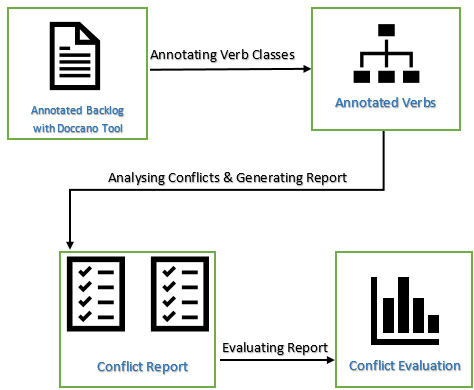
\includegraphics[scale=0.65]{conflict_operational_flow}
	\caption{Step-by-step visualisation of the tool chain and its inputs and outputs}\label{fig:conflict_operational_flow}
\end{figure}
\paragraph{Preparing the JSON-Format of the Primary Input}\label{conflict_workflow_preparing_json_format}
Since the annotated USs in the original JSON files did not separate entries such as Entity, Action, Text, Targets and Contains, it is not clear which element belongs to which part of the USs, which leads to ambiguity. Accordingly, we use a class called \textit{JSONTransformer} that separates entries based on their occurrence in both the main and benefit parts of the USs. It also specifies an identifier to assign a unique identifier to each US, which is stored in a JSON object called \textit{"US\_Nr"}. 
These additions improve the system's ability to distinguish and process individual USs within the analytical pipeline.

\paragraph{Extraction of text reports} Creating a text report aims to find conflicts between USs and highlight important information, such as identifying potentially conflicts US-pairs, the conflict reason, the resource (as noun) affected by actions (as verbs) causing the conflict, the texts of the main parts with the affected elements marked with \# and a tabulation of the potentially conflicting pairs.

\paragraph{Evaluating the reports} Once we have created the reports, we can now assess the correctness of the US-pairs reported as conflicts, i.e. whether the reported US-pairs really cause a conflict.

\subsubsection*{Software Architecture}\label{conflict_architectur}
In this section, we present the basic structures of our workflow and the discipline of creating such structures. Each structure comprises software elements, relations among them, and properties of both.
\begin{itemize}
	\item Annotated USs with Doccano Tool\footnote{https://github.com/doccano/doccano}: Mosser et al. used publicly available requirements from Dalpiaz et al.\cite{Dalpiaz2018} consisting of 19 product backlogs and 1,458 USs. The dataset is a raw archive of 19 text files, each containing one US per line. As there were no public expert-based annotations, Mosser et al. manually annotated the dataset using the Doccano tool for \textit{Named Entity Recognition}. Labels included persona, action, entity, benefit part and relations such as triggers, targets, and contains based on their domain meta-model.
	As artefact we receive a graph-based model with JSON format, which represents the refined and annotated dataset for the recognition of \emph{entities}, \emph{actions}, \emph{personas} and \emph{benefits} of USs \cite{mosser2022modelling}.
	
	\item Eclipse as IDE\footnote{https://eclipseide.org/}: Eclipse is an integrated development environment (IDE) used in computer programming. It contains a base work workspace and an extensible plug-in system for customizing the environment.
	We chose this IDE because it offers the Henshin tool specifically for model-based development.
	
	\item VerbNet as Verb Lexicon Resource\footnote{https://verbs.colorado.edu/verbnet/}: VN is the largest on-line network of English verbs that links their syntactic and semantic patterns. It is a hierarchical, domain-independent, broad-coverage verb lexicon with mappings to other lexical resource, such as WordNet\footnote{https://wordnet.princeton.edu/}, PropBank \footnote{https://propbank.github.io/}, and FrameNet \footnote{http://framenet.icsi.berkeley.edu/}. VerbNet is organized into verb classes extending Levin (1993) classes through refinement and addition of subclasses to achieve syntactic and semantic coherence among members of a class. Each verb class in VN is completely described by thematic roles, selectional preferences of the arguments, and frames consisting of a syntactic description and a semantic representation with subevent structure patterned on the Dynamic Event Model of Pustejovsky and Moszkowicz and Pustejovsky\cite{kipper2006extending}.
	
	\item JSONTransformer Class: This class is part of the \textit{org.henshin.backlogconflict.code.rule} package and is a key component of the software architecture designed for transforming primary input datasets in JSON format. It separates entries based on their occurrence in both the main and benefit parts of the USs. It also assigns a unique identifier to each US to facilitate tracking and management. 
	
	This transformation simplifies subsequent tasks for editing, analysing and conflict resolution by providing a clear structure for the USs and their components. The separation of main and benefit parts and the assignment of unique identifiers improves the manageability and traceability of USs within the system.
	
	\item Action Rule Reference Database: This component is essential for identifying conflicts between USs, especially conflicts arising from actions over common entities ( as resources). To achieve this, we categorise actions into four different groups: \textit{Preserve, Delete, Create and Prohibit}.
	
	The main purpose of the action rule reference database is to facilitate the translation of actions (in the form of verbs) found in USs into corresponding action-rules. This process involves several important steps:
	\begin{enumerate}
		\item Collection of Actions: We collect all actions (represented as verbs) from existing datasets and compile them into a CSV file. This file serves as comprehensive reference database.
		
		\item Contextual Translation: Each verb in the CSV file is translated into the corresponding action-rules related to its VerbNet class. 
	\end{enumerate}
	
	\item ActionsRulesCreator Class: The ActionsRulesCreator class is an integral part of the \textit{org.henshin.backlogconflict.code.rule} package. It leverages the action rule reference database to enhance the JSON transformation process by adding new \textit{target} JSON-Array entries. These entries consist of a set of triples: action, entity, and action-rules. The action-rules are derived from the reference database, ensuring consistent and accurate conflict detection and resolution.
	
	\item ReportMaker Class: This class developed within the \textit{org.henshin.backlogconflict .code.report} packages, its primary function is to identify conflicting US-pairs based on specific criteria and generate comprehensive reports on these conflicts. This class provides detailed information on the nature of the conflicts, making it an invaluable tool for maintaining system coherence and resolving inconsistencies. It performs the following key tasks:
	\begin{enumerate}
		\item Identification of Conflict US-pairs: The class analysis USs to identify pairs that conflict based on predefined criteria. These criteria may including conflicting actions, or inconsistencies in the USs.
		
		\item Detailed Conflict Reporting: Once conflicts are identified, the class generates detailed reports. These reports contain essential information such as the affected entity(as resource), potential conflicted actions, conflict reason, and the texts of main parts of the USs with marked elements with "\#".
		
		\item Tabular Summary: In addition to detailed conflict descriptions, the class also produces a tabular summary of all identified conflict pairs in a backlog, providing a quick overview of the conflict US-pairs.
	\end{enumerate}
	
	\item ReportExtractor Class: The class from the \textit{org.henshin.backlog.code.report} package is used in our software architecture to extract and format reports from the CDA-generated \textit{Minimal-Model.ECore} that contain all information about redundant US-pairs such as redundant elements with their name and type. It uses classes from the \textit{org.eclipse.emf.ecore} package to handle EMF (Eclipse Modelling Framework) resources that support the management and manipulation of \textit{Minimal-Model.ECore} data in a structured format.
	
	In operation, the ReportExtractor class reads minimal-model.ecore files containing detailed information about redundant US-pairs. It then processes this data to generate reports in both text and JSON formats, aiding in the systematic analysis of potential redundancies within the USs. This is facilitated through methods that dynamically read and interpret the JSON data, extracting key information such as actions, entities, and their interactions.
	
	\item Evaluation Class: The class is part of the \textit{org.henshin.backlog.code.evaluation} package, serves a critical function within our software architecture, focusing on the analysis and determination of redundancy between USs based on specified criteria. This class utilizes JSON processing to assess the overlap and redundancy between elements of USs, such as triggers, targets, and contains, which are vital for identifying potential redundancies in the USs.
	
	Key functionalities of this class include reading and interpreting JSON data, where it extracts detailed elements related to USs and evaluates them against redundancy criteria defined in its methods. The class's method \textit{evaluateRedundancyCriteria} is particularly central, as it processes the JSON objects representing USs to determine if they are fully or partially redundant based on the presence and matching of various JSON array elements like triggers, targets, and contains in the main and benefit parts of the USs.
	
\end{itemize}
Figure \ref{fig:conflict_technical_implementation} shows the architectural composition, highlighting the integral components and their user interface and artefacts.
\begin{figure}[h]
	\centering 
	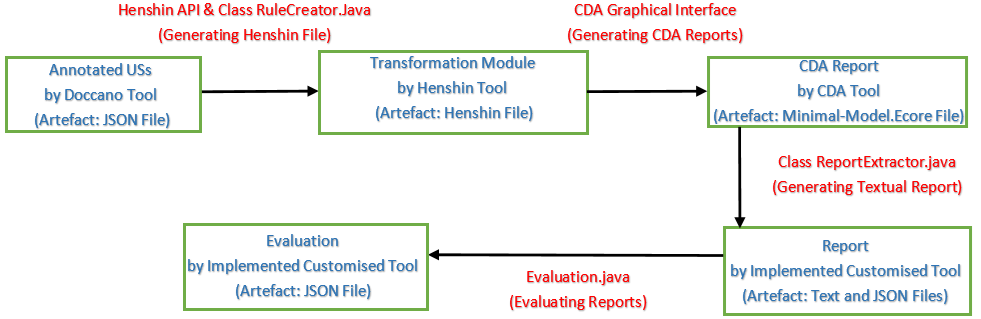
\includegraphics[scale=0.6]{technical_implementation}
	\caption{Design phases}\label{fig:conflict_technical_implementation}
\end{figure}
Regarding conflict, some definitions are clarified:
\begin{definition}[\textbf{Main and Benefit Parts in User Story}]
	A user story (US) is divided into two distinct parts that collectively describe what the user wants, why they want it, and how it will benefit them. These are:
	\begin{itemize}
		\item The \textit{main part}, which is essential as it clearly and concisely summarises the persona, the intended functionality and the resources required to perform the action. This part usually has follow the format: \textit{"As a [persona], I want [what]"}. 
		
		Here, the persona helps contextualise the requirement by linking it to a user type, which promotes understanding and empathy. The intended functionality describes the action that the persona wants to perform or the function they need, providing a clear statement of the requirement.
		
		Specifying the resources required to perform the action helps with planning and resource allocation and ensures that the development team is aware of the tools, technologies and time required.
		
		\item The \textit{benefit part}, which formulates the potential benefit for the end user and typically begins with the phrase \enquote{so that}. This part of the US is used for justifying the need for a feature by explaining the value or improvement it brings to the user's experience. It connects the functionality directly to user satisfaction, efficiency, or productivity gains, making it easier for the development team to prioritize features based on their impact.
		
		It is worth noting that sometimes the benefit part may not exist in the structure of USs. In such cases, the main part can stand alone.
	\end{itemize}
\end{definition}
\newpage
\begin{definition}[\textbf{Conflict}]
	 %TODO: angepasste US
	Conflict refers to situations where two USs try to:	 
	\begin{itemize}
		\item delete a resource which another US are using
		\item delete a resource which another US also wants to delete
		\item create a resource which another US prohibits
	\end{itemize}
	$Notation$. Lowercase identifiers refer to single elements, and uppercase identifiers denote sets. 
	\\A user story $us$ is a 2-tuple $us = \langle m,b\rangle $ where:
	\begin{enumerate}
		\item A main $m$ is define a 6-tuple: \\\\$m = \langle p,A,E,Tr,Ta,Co\rangle $ \\\\where:
		
	\begin{itemize}
		\item $p$ is the persona.
		
		\item $A = \{ a_1,a_2,...\} $ is a set of actions.
		
		\item $E = \{e_1,e_2,...\}$ is a set of entities.
		
		\item $Tr = \{(p_1,a_1),(p_2,a_2),...\}$ is a set of trigger references, each begin a pair of persona and action.
		
		\item $Ta = \{(a_1,e_1,R_1),(a_2,e_2,R_2),...\}$ is a set of target references, each begin a triple of action, entity, and action-rules $R$.
		
		\item $Co = \{ (e_1,e_2,R_1),(e_*,e_*,R_2),... \}$ is a set of contain references, each begin a triple of entities and action-rules R.
		
		\item $R = \{preserve, create, delete, forbid\}$ are the rules applied to actions.
	\end{itemize}
		\item A benefit $b$ is define as a 4-tuple:\\\\ $b = \langle A,E,Ta,Co\rangle $\\\\ where: 
		\begin{itemize}
			\item $A = \{ a_1,a_2,...\} $ is a set of actions.
			 
			\item $E = \{e_1,e_2,...\}$ is a set of entities.
			
			\item $Ta = \{(a_1,e_1),(a_2,e_2),...\}$ is a set of target references, each begin a pair of action and entity.
			
			\item $Co = \{ (e_1,e_2),(e_*,e_*),... \}$ is a set of contain references, each begin a pair of entities. 
			
		\end{itemize}
	\end{enumerate}
	To denote that a syntactic operator, we add the subscript
	“syn”; for instance, $=_{syn}$ is syntactic equivalence which introduced by Lucassen et al. \cite{lucassen2016improving}.\\ Consider two USs:\\\\ $us_1 = \langle m_1,b_1\rangle $ where $m_1 = \langle p_1,a_1,e_1,tr_1,ta_1,co_1 \rangle$\\\\$us_2 = \langle m_2,b_2\rangle$ where $m_2 = \langle p_2,a_2,e_2,tr_2,ta_2,co_2 \rangle$ \\\\
	$us_1$ causes a conflict if:\\\\ The entity $e_1$ is an exact redundant of entity $e_2$, formally:\\ $isRedundant(e_1,e_2) \leftrightarrow e_1 =_{syn} e_2$ and one of the following conditions holds:\\
	\begin{enumerate}
		\item $ta_1 = (e_1,a_1,"preserve")$ and $ta_2 = (e_2,a_2,"delete")$
		
		\item $ta_1 = (e_1,a_1,"create")$ and $ta_2 = (e_2,a_2,"forbid")$
		
		\item $ta_1 = (e_1,a_1,"delete")$ and $ta_2 = (e_2,a_2,"delete")$
	\end{enumerate}
	To comprehensively assess conflicts, it is important to consider not only the textual content but also the functional relevance of each action over entities within the USs. By categorizing actions into four groups, conflict that may not be immediately apparent through a simple text comparison can be uncovered, thereby reducing time consumed in finding conflicts manually.
\end{definition}	
\begin{definition}[\textbf{Full Redundancy}]
	A US-pair are fully redundant in their main parts if
	\begin{itemize}
		\item there are redundant target references $Ta_2$ in $m_2$ for all target references $Ta_1$ in $m_1$, so that $Ta_1$ and $Ta_2$ are redundant, and vice versa, and
		
		\item there are redundant trigger references $Tr_2$ in $m_2$ for all trigger references $Tr_1$ in $m_1$, so that $Tr_1$ and $Tr_2$ are redundant, and vice versa, and
		
		\item there are redundant contain references $Co_2$ in $m_2$ for all contain references $Co_1$ in $m_1$, so that $Co_1$ and $Co_2$ are redundant, and vice versa.
		
	\end{itemize}
	A US-pair are fully redundant in their benefit parts if
	\begin{itemize}
		\item there are redundant target references $Ta_2$ in $b_2$ for all target references $Ta_1$ in $b_1$, so that $Ta_1$ and $Ta_2$ are redundant, and vice versa, and
		
		\item there are redundant contain references $Co_2$ in $b_2$ for all contain references $Co_1$ in $b_1$, so that $Co_1$ and $Co_2$ are redundant, and vice versa.
		
	\end{itemize}
	A US-pair was categorised as "full redundancy" in the main/benefit part if all occurring clauses in the main/benefit part consisting of triggers (for the main part only), targets and contains were syntactically identical.\\\\
	This means that in each pair, the wording, order and structure of the clauses relating to the triggers and targets must be identical to fall into this category. The check also extends to the "contain" elements, if these are present, to ensure that these also match perfectly and without deviations.\\\\
	Full redundancy in the main part means that the redundant stories do not provide additional information and can be consolidated or eliminated without compromising the completeness or operational integrity of the system specifications.\\\\
	On the other hand, having this level of redundancy in the benefit part means that USs achieve the same goal; they can be categorised in the same group. This means that if the end results or benefits described by the USs are identical, regardless of the different actions/entities or triggers that lead to these results, the USs effectively serve the same purpose within the system.
\end{definition}
\begin{example}
	For example, the following US-pair is identified as \enquote{Full Redundancy} in the main part:
	
	\textit{user\_story\_01:} \enquote{\#g14\# as a \#publisher\#, i want to \#publish\# a \#dataset\#, so that i can view just the dataset with a few people.}
	
	\textit{user\_story\_02:} \enquote{\#g14\# as a \#publisher\#, i want to \#publish\# a \#dataset\#, so that i can share the dataset publicly with everyone.}\\\\
	All existing clauses associated with the main elements in this scenario - in particular the trigger (where "Publisher" is the persona and "Publish" is the action) and the targets (where "Publish" is the action and "Dataset" is the entity) - are exactly the same in the main parts of the USs. This complete similarity shows that there is "full redundancy" in the main parts of these USs.
\end{example}
\begin{example}
	Following US-pair is identified as \enquote{Full Redundancy} in \enquote{Benefit} part:
	
	\textit{user\_story\_02:} \#g05\# as a data publishing user, I want to be able to edit the model of data I have already imported, so that I can \#fix\# \#bugs\# or \#make\# \#enhancements\# in the \#API\# built for my \#data\#.
	
	\textit{user\_story\_07:} \#g05\# as a data publishing user, I want to be able to edit the data source of data I have already imported, so that i can \#fix\# \#bugs\# or \#make\# \#enhancements\# in the \#API\# built for my \#data\#.
	
	As we can see, targets(["fix", "bugs"], ["make", enhancements"]) and contains (["API", "enhancements"], ["data","API"]) in the benefit part are identical between USs, therefore, we have \enquote{Full Redundancy} in the \enquote{Benefit} parts.
\end{example}
Last but not least, sometime there are words in the annotated USs that are not labelled as a reference (trigger, target or contain) by the Doccano tool at all, which leads to a full redundancy being incorrectly recognised instead of a partial.
\begin{example}
	Considering following US-pair:
	
	user\_story\_26: \#g05\# as an \#api user\#, i want to be able to \#understand\# if a \#user\# is an administrator, so that [...].
	
	user\_story\_25: \#g05\# as an \#api user\#, i want to be able to \#understand\# if a \#user\# is a publisher, so that [...].\\\\
	In this example, full redundancy is found due to the redundant targets and triggers in the main part, which is not entirely correct. This is because there are some phrases that do not appear as contain or target in any reference, such as: "administrator" (user\_story\_26) and "publisher" (user\_story\_25).
\end{example}
\begin{definition}[\textbf{Partial Redundancy}]
	A US-pair are partially redundant in their main parts if there is a target reference $ta_1$ in $m_1$ and a target reference $ta_2$ in $m_2$, so that $ta_1$ and $ta_2$ are redundant.\\\\
	A US-pair are partially redundant in their benefit parts if there is a target reference $ta_1$ in $b_1$ and a target reference $ta_2$ in $b_2$, so that $ta_1$ and $ta_2$ are redundant.\\\\
	Note that in this definition, a US-pair that is fully redundant in the main part (or in the benefit part) is also partially redundant in the main part (or in the benefit part).\\\\
	Partial redundancy in USs occurs when only certain clauses, such as targets, have significant overlap but are not completely identical. This means that while there are shared aspects such as targets between USs, other clauses such as triggers or contains may not overlap, indicating an incomplete match. Such a scenario indicates that there is substantial, but not fully, a match between the USs.
	%	Was found when only some clauses were redundant in either the Main or Benefit parts, while others were unique. This indicates overlapping clauses, but not full redundancy.
\end{definition}
\begin{example}
	Following US-pair is identified as \enquote{Partial Redundancy} in main part:
	
	\textit{user\_story\_09:} \#g04\# as a \#user\#, I want to be able to \#view\# a \#map display\# of the public recycling bins around my \#area\#.
	
	\textit{user\_story\_10:} \#g04\# as a \#user\#, I want to be able to \#view\# a \#map display\# of the special waste drop off sites around my \#area\#.
	
	As we can see, there are some redundancy clauses such as Triggers (["user", "view"]), Targets (["view", "map display"]) and Contains(["map display", "area"]) between the USs. There are also clauses such as Contains (["public recycling bins"] vs. ["hazardous waste collection points"]) that are distinct elements justifying the maintaining of separate USs. We therefore assess this as "Partial redundancy" in the "Main part".
\end{example}
\begin{example}
	Following US-pair is identified as \enquote{Partial Redundancy} in benefit part:
	
	\textit{user\_story\_17:} \#g03\# as a staff member, I want to manage approved proffers, so that I can \#ensure\# \#compliance\# with and satisfaction of the proffer in the future.
	
	\textit{user\_story\_30:} \#g03\# as a staff member, I want to manage affidavits, so that I can \#ensure\# \#compliance\# with the requirements prior to the hearing.
	
	As we can see, there is a redundancy clause as targets (["ensure", "compliance"]) between the USs in the benefit part, but there is also a clause as contains (["proffer", "satisfaction"] vs ["requirements", "hearing"]), which leads us to evaluate this as \enquote{Partial Redundancy} in the \enquote{Benefit} part.
\end{example}
\subsubsection*{Design Phases}\label{design_phases}
To provide a comprehensive overview of the design phases, this section explains each step of the process, from initial setup to final evaluation, using practical examples.
\subsubsection*{Step 1: Data Preparation}\label{design_step_1}
As primary input, we receive a graph-based model generated by the Doccano tool, which represents the refined and annotated dataset for the recognition of \emph{entities}, \emph{actions}, \emph{persons} and \emph{benefits} of USs \cite{arulmohan2023extracting}.

The datasets have the JSON format, the structure of which is very important in the Java classes \textit{RuleCreator}, \textit{ReportExtractor}, and \textit{Evaluation}. Therefore, understanding the JSON format provided is needed for the further procedure.

Each JSON file for a backlog dataset contains a JSON-array in which each US entry is defined as a JSON-object. Listing \ref{list:desing_json_format} illustrates the format used for the US entry.
\begin{MyListing}
	\paragraph{}
	\hrule
	\centering
	\lstinputlisting[basicstyle=\ttfamily\footnotesize]{Listing/json_format.json}
	\caption{The JSON format of each US entry in JSON file}\label{list:desing_json_format}
	\hrule
\end{MyListing}
Mosser et al. have linked each \emph{Persona} to each \emph{Primary Action} as \emph{Trigger} relationships, each \emph{Primary Actions} to each \emph{Primary Entity} as \emph{Target} relationships and each \emph{Primary/Secondary Entity} to each \emph{Primary/Secondary Entity} implying a \emph{Contains} relationship\cite{arulmohan2023extracting}.

To interact with the entries in JSON file, we need to distinguish between the entries that are defined as JSON-objects, such as: {Text, Action, Entity, Benefit} and the entries that are defined as a JSON-array, such as: {Persona, Primary/Secondary Action, Primary/Secondary Entity, Triggers, Targets, Contains}.
\subsubsection*{Identifying USs in JSON-File}\label{desing_workflow_nummerize_us}
Annotated USs in each JSON file have no identifier. To distinguish USs, we use a Python script called \textit{nummerise\_us.py} \footnote{https://github.com/amirrabieyannejad/Redundancy\_Analysis/tree/main/Script/numberise\_us}, which receives JSON files as input and adds a JSON object named \enquote{US\_Nr} with an identifier as value (e.g. user\_story\_01) to each US and returns the JSON files as output.
Listing \ref{list:desing_json_format_sample} illustrates the added JSON object "US\_Nr" and its value in the JSON file.
\begin{MyListing}
	\paragraph{}
	\hrule
	\centering
	\lstinputlisting[basicstyle=\ttfamily\footnotesize]{Listing/json_format_sample.json}
	\caption{The JSON format with the additional JSON object "US\_Nr" and its value}\label{list:desing_json_format_sample}
	\hrule
\end{MyListing}
\subsubsection*{Step 2: Creation of Rules}\label{design_step_2}
Step 2 of the design involves a central process in which the US data structured in JSON files is transformed into transformation rules using the Henshin API. This involves the creation of an Ecore meta-model that represents the structure of the data we are working with, followed by the generation of Henshin transformation rules using RuleCreator class.
\subsubsection*{Creating Ecore Meta-Model}\label{design_workflow_ecore}
To be able to create rules in Henshin, an Ecore (meta)-model should be available. Ecore is the core (meta)-model at the heart of the EMF (Eclipse Modelling Framework). It enables the formulation of other models by utilising its constructs.

Accordingly, we create an Ecore meta-model as shown in Figure \ref{fig:design_ecore_meta_model}, which is inspired by the meta-model shown in Figure \ref{fig:conceptual_metamodel} and corresponds to the JSON-objects in the JSON-file as follows:
\begin{itemize}
	\item \textit{Persona} as a class in the meta-model corresponds to the JSON-object \enquote{Persona} in the JSON-file.
	\item \textit{Entity} as an abstract class, from which \textit{Primary/Secondary Entity} inherits as a class in the meta-model, corresponds to the JSON-object \enquote{Entity}, which contains two JSON-arrays, namely \enquote{Secondary/Primary Entity} in the JSON-file.
	\item \textit{Action} as an abstract class and \textit{Primary/Secondary Action} as an inherited class in the meta-model correspond to the JSON-object \enquote{Action}, which contains two JSON-arrays, namely \enquote{Secondary/Primary Action} in the JSON-file.
	\item \textit{Benefit} as a class in the meta-model, which also has an attribute called \enquote{text} that corresponds to the JSON-object \enquote{Benefit} in the JSON-file.
	\item \textit{Story} as a class in the meta-model that contains text from US, which also has an attribute called \enquote{text} that corresponds to the JSON-object \enquote{Text} in the JSON-file.
	\item Abstract class \textit{NamedElement} has attribute \textit{name}, which Primary/Secondary Action/Entity inherit from it, which corresponds to the value of \textit{Primary/Secondary Action/Entity} in JSON-file.
	\item \textit{Edge} with the name \textit{triggers} between Persona and Primary Action in the meta-model, which corresponds to the JSON-array \enquote{Triggers}, where each JSON-array in it contains a pair, the first element corresponding to the \textit{Persona} and the second to the \textit{Primary Action}.
	\item \textit{Edge} named \textit{targets} between Primary/Secondary Action and Primary/Secondary Entity in the meta-model, which corresponds to the JSON-array \enquote{Targets}, where each JSON-array has a pair, the first element corresponding to \enquote{Primary/Secondary Action} and the second element corresponding to \enquote{Primary/Secondary Entity}.
	\item \textit{Edge} named \textit{contains} between Primary/Secondary Entity and itself in the meta-model, which corresponds to the JSON-array \enquote{Contains}, where each JSON-array in it has a pair where the first element corresponds to \enquote{Primary/Secondary Entity} and the second element corresponds to \enquote{Primary/Secondary Entity}.
\end{itemize}
\begin{figure}[h]
	\centering
	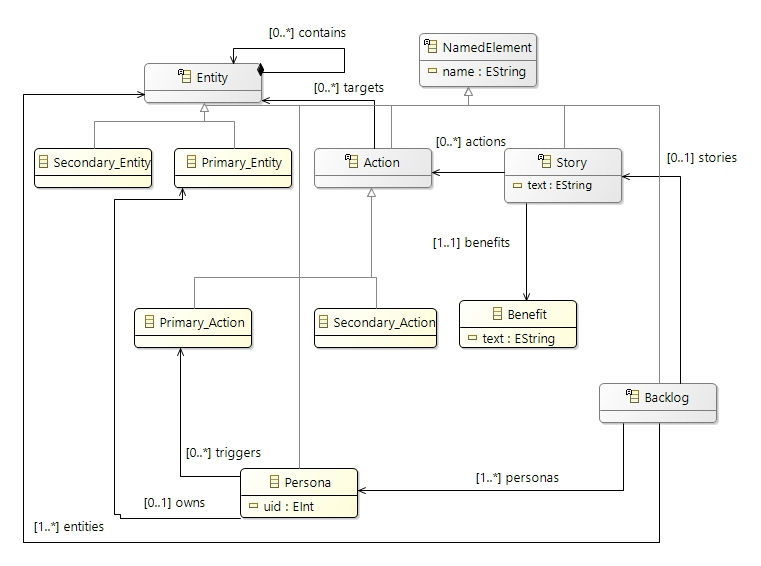
\includegraphics[scale=0.6]{ecore_metamodel}
	\caption{Ecore meta-model inspired by Mosser et al. \cite{mosser2022modelling}}\label{fig:design_ecore_meta_model}
\end{figure}
\subsubsection*{Creating Rules}\label{design_workflow_rule_creator}
With the identified USs in the the JSON-file, we generate rules with the Henshin package \textit{org.eclipse.emf.henshin.model.compact}, which is responsible for the creation of \textit{transformation rules} and their \textit{classes}, \textit{attributes}, \textit{edges} and annotates them with \textless\emph{Delete}\textgreater, \textless\textit{Create}\textgreater or\textless\textit{Preserve}\textgreater, which are vital for the CDA tool to recognise the redundant pairs.

To generating rules we create a package named \textit{org.henshin.backlog.code.rule} and specially the class \textit{RuleCreator} which used following classes\footnote{https://wiki.eclipse.org/Henshin/Compact\_API}:
\begin{itemize}
	\item \textit{org.eclipse.emf.henshin.model.compact.CModule}: CModule class can import elements from an Ecore file to use them in the transformation process responsible for linking the Ecore meta-model to the Henshin-file to be created.
	\item \textit{org.eclipse.emf.henshin.model.compact.CRule}: Once we have a CModule, we can specify transformation rules with the CRule class and create them.
	\item \textit{org.eclipse.emf.henshin.model.compact.CNode}: Now that we have a transformation rule, we want to fill this rule with nodes, edges and attributes. To create a node within a transformation rule, we need the CRule class. To create an edge we need to reference two nodes together. The default action when specifying a node, edge or an attributes is the \textless\emph{preserve}\textgreater action. We can also specify a different action when we create a node or an edge, for example \textless\emph{delete}\textgreater or\textless\emph{create}\textgreater.
	\item org.henshin.backlog.code.rule.RuleCreator: We implement \textit{RuleCreator} class that creates a rule with annotated nodes, edges and attributes based on a JSON-file as input and a Henshin-file containing all rules as output, where each rule and its members(nodes, attributes, edges) correspond to the individual US and their JSON-objects/arrays in the JSON-file. 
	
	The most important design decision of this class is the way nodes, attributes and edges are annotated in order to be able to apply conflict and dependency analysis (CDA) for rules stored as a Henshin file.
	
	We decided to annotate the \enquote{name} attribute of all Primary/Secondary Actions/Entities and their associated edges including \enquote{targets}, \enquote{triggers} and \enquote{contains} as \textless delete\textgreater  action. 
	
	The main goal is to increase the probability of identifying US-pairs characterised by matching names of \textit{action} nodes and \textit{entity} nodes in conjunction with an edge called \textit{targets}. This congruence serves as a basic criterion for identifying potentially redundant US-pairs and simplifies the process of redundancy detection in the context of US analysis.
\end{itemize}
\begin{example}
	Listing \ref{list:design_json_user_story_12} shows the JSON format in relation to user\_story\_12 and Figure \ref{fig:desing_rule_user_story_12} shows the application of the RuleCreator class in this US, which is a transformation rule where the targets and the associated contains relationships are annotated as a \textless Delete\textgreater action and the rest of the nodes and edges are annotated as a \textless Preserve\textgreater action.\\\\
	Text of US is:
	user\_story\_12: "\#G03\# As a Staff member, I want to Assign an Application for Detailed Review, so that I can review the for compliance and subsequently approved or denied."
	%Considering the backlog dataset as shown in Listing \ref{list:backlog_g03}:
	\begin{MyListing}
		\paragraph{}
		\centering
		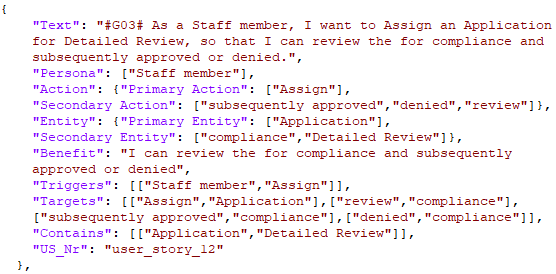
\includegraphics[scale=0.8]{Listing/json_user_story_12.png}
		\caption{JSON entities Related to user\_story\_12}\label{list:design_json_user_story_12}
	\end{MyListing}
	\begin{figure}[h]
		\centering
		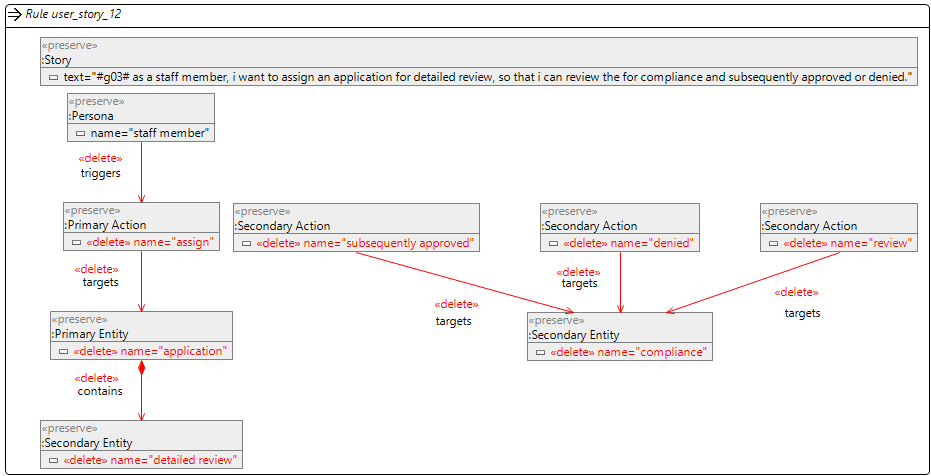
\includegraphics[scale=0.6]{rule_user_story_12}
		\caption{Generated transformation rule related to user\_story\_12 using RuleCreator class}\label{fig:desing_rule_user_story_12}
	\end{figure}
	As we can see, the "targets" edges and their direct relationships ("triggers" and "contain", if any) are also annotated as \textless delete\textgreater, which is very important to find redundant elements with the CDA tool.
\end{example}
\begin{example}
	Listing \ref{list:design_json_user_story_39} shows the JSON entities related to user\_story\_39 and Figure \ref{fig:design_rule_user_story_39} shows transformation rule generated by RuleCreator class.\\\\
	Text of US is:
	user\_story\_39: "\#G03\# As a Plan Review Staff member, I want to Review Plans, so that I can review them for compliance and either approve, or fail or deny the plans and record any conditions, clearances, or corrections needed from the Applicant."
	\begin{MyListing}
		\paragraph{}
		\centering
		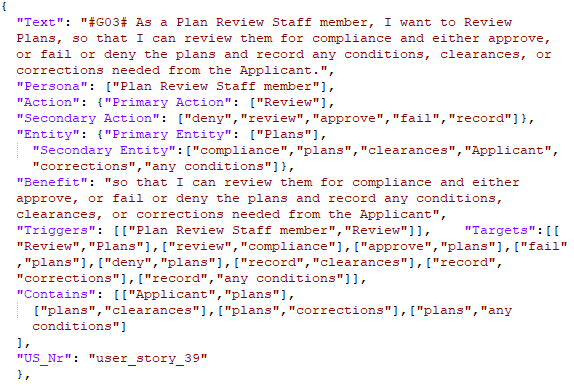
\includegraphics[scale=0.8]{Listing/json_user_story_39.png}
		\caption{JSON entities Related to user\_story\_39}\label{list:design_json_user_story_39}
	\end{MyListing}
	\begin{figure}[h]
		\centering
		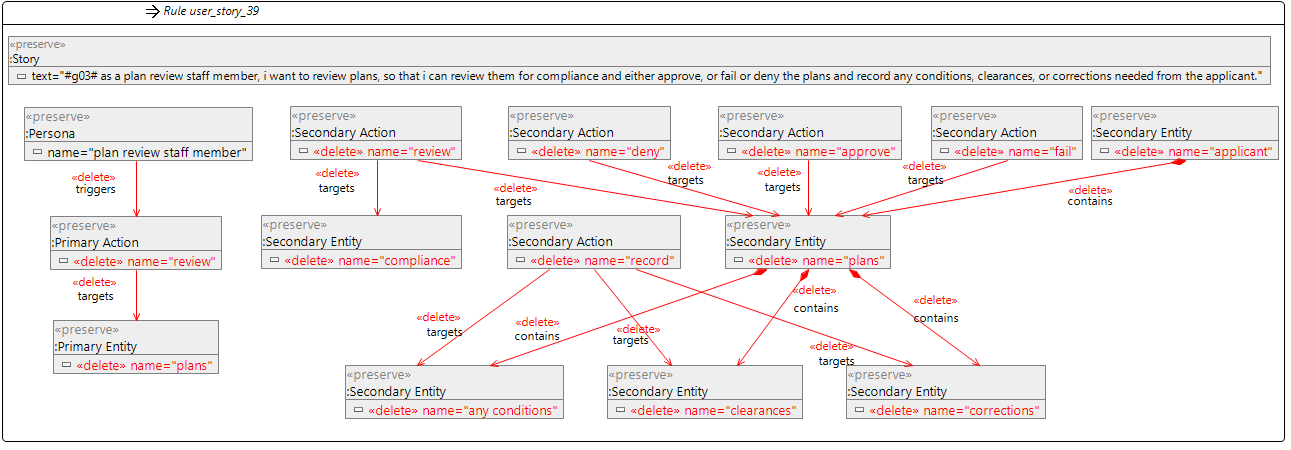
\includegraphics[scale=0.43]{rule_user_story_39}
		\caption{Generated transformation rule related to user\_story\_39 using RuleCreator class}\label{fig:design_rule_user_story_39}
	\end{figure}
	Attribute "Plan", as we can see, it appears both in the main part as a primary entity and in the benefit part as a secondary entity, forming the various relationships as targets and contains.
\end{example}
\begin{example}
	Listing \ref{list:desing_json_user_story_51} shows the JSON entities related to user\_story\_51 and Figure \ref{fig:desing_rule_user_story_51} shows transformation rule generated by RuleCreator class.\\\\
	Text of US is:
	user\_story\_51: "\#G03\# As an Enforcement Staff member, I want to Issue a Notice of Violation, so that I can provide formal communication to the responsible party."
	\begin{MyListing}
		\paragraph{}
		\centering
		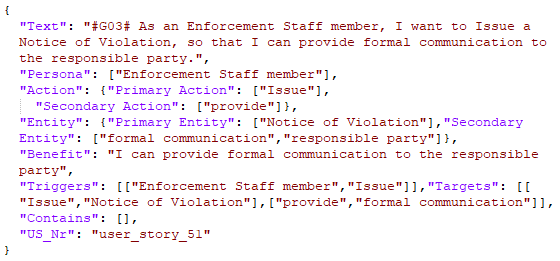
\includegraphics[scale=0.8]{Listing/json_user_story_51.png}
		\caption{JSON entities Related to user\_story\_51}\label{list:desing_json_user_story_51}
	\end{MyListing}
	\begin{figure}[h]
		\centering
		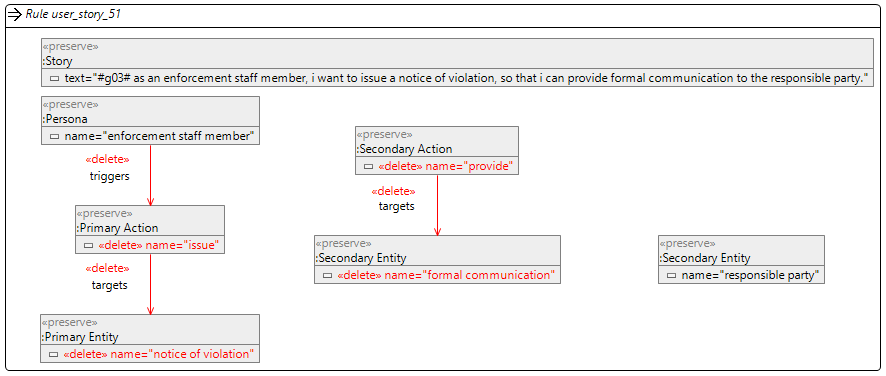
\includegraphics[scale=0.55]{rule_user_story_51}
		\caption{Generated transformation rule related to user\_story\_51 using RuleCreator class}\label{fig:desing_rule_user_story_51}
	\end{figure}
	Last but not least, we have determined that the secondary entity "responsible party" has neither a target nor a contains relationship. Therefore, it is not annotated as \textless delete\textgreater, but as \textless preserve\textgreater. This is due to the fact that some phrases have been identified as entities in the Doccano tool, but their relationship is not annotated at all, which is problematic for analysing redundancy.
\end{example}
\subsubsection*{Step 3: Conflict and Dependency Analysis}\label{step_3}
After the rules and the corresponding henshin file have been created by the RuleCreator class, we are now able to pass them to the conflict and dependency analysis (CDA) to find potential redundancy pairs.

Since the analysis of conflicts and dependencies related to the \textit{attribute} is not yet considered in the CDA API \footnote{https://wiki.eclipse.org/Henshin/conflict\_and\_Dependency\_Analysis}, we decided to use the user interface (UI) of the CDA extension of Henshin, which supports analysis of conflict and dependencies of rules through the interactive use of CDA.

To apply CDA to Henshin files, we just need to right-click on the Henshin file and select \textit{Henshin} -\textgreater\textit{ conflict and Dependency Analysis} from the context menu as shown in Figure \ref{fig:henshin_context_menu}.
\begin{figure}[h]
	\centering
	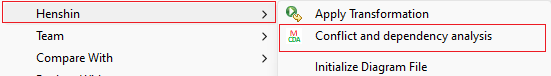
\includegraphics[scale=0.5]{henshin_context_menu}
	\caption{Applying CDA to the selected Henshin file}\label{fig:henshin_context_menu}
\end{figure}
A user interface then appears, prompting to select the rule sets to be analysed and the type of analysis. We then select as \enquote{\textit{First}} and \enquote{\textit{Second} \textit{Rules}}, all rules related to USs. Additionally, as the type of analysis we select \enquote{\textit{conflicts}} as illustrated in Figure \ref{fig:select_rules}.
\begin{figure}[h]
	\centering
	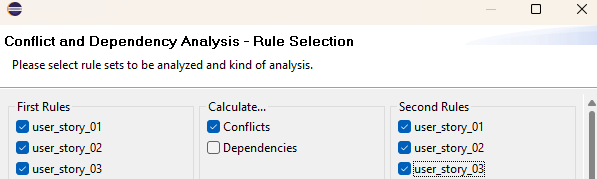
\includegraphics[scale=0.5]{select_rules}
	\caption{CDA user interface: Selection of rules and type of analysis}\label{fig:select_rules}
\end{figure}
On the next page of the CDA UI shown in Figure \ref{fig:select_granularity}, we specify the depth of analysis that we use with \enquote{\textit{Fine granularity}} when selecting \enquote{\textit{Create a complete result table}} and \enquote{\textit{Create an abstract result table}}. 

Fine granularity provides a detailed examination of each conflicting rule by listing all conflict reasons. Unlike coarse granularity, which focuses only on minimal conflict reasons, fine granularity includes both minimal and more general conflict reasons. The binary granularity, where simple conflicting rule pairs are listed, may be too simple for complex systems where understanding the nature of the conflict is essential for the solution. 
We choose \enquote{Fine granularity} as the depth of analysis due to the fact that it shows all conflict reasons for each conflicting rule pair. This allows for a deeper understanding of how different model fragments contribute to conflicts.

A conflict reason is a model fragment whose presence leads to a conflict. General conflict reasons result from different combinations of minimal conflict reasons\cite{cda_api}.
\begin{figure}[h]
	\centering
	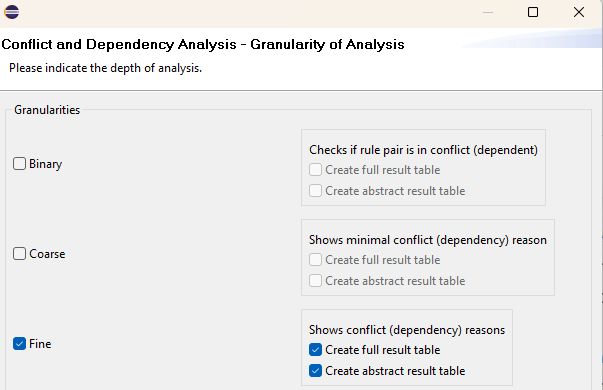
\includegraphics[scale=0.5]{select_granularity}
	\caption{CDA user interface: Selection of report granularity}\label{fig:select_granularity}
\end{figure}
During the execution of the CDA analysis, the rule pairs is analysed and a conflict analysis is performed. Once the calculation is complete, the results are listed in the \enquote{CDA} -\textgreater \enquote{Result window}, as shown in Figure \ref{fig:cda_report}. The top entry shows the granularity, which in our case is \enquote{Fine}. These entries contain the rule pairs that conflict with each other. Each rule pair contains a number of conflict reasons.
\begin{figure}[h]
	\centering
	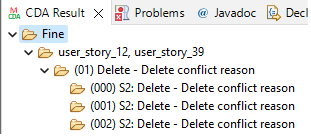
\includegraphics[scale=0.5]{cda_report}
	\caption{CDA report with fine granularity}\label{fig:cda_report}
\end{figure}
Figure \ref{fig:cda_report_in_project_dir} shows how the data is saved in the project tree view. The results directory is created in the directory containing the Henshin that was used for the analyses. The new folder name is the date and time at which the analysis was performed. In contrast to the \enquote{\textit{CDA/Results}} view, this folder contains all conflict reasons and atoms together in a rule pair directory.
\begin{figure}[h]
	\centering
	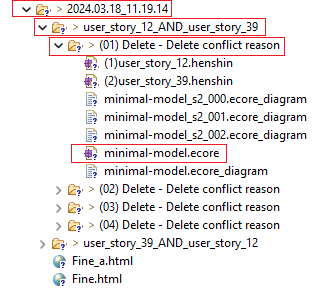
\includegraphics[scale=0.5]{cda_report_in_project_dir}
	\caption{Saving CDA results data in the project structure view}\label{fig:cda_report_in_project_dir}
\end{figure}
For each conflict reason, there is a \enquote{\textit{minimal-model.ecore}} file, that contains packages in which various conflict elements such as \enquote{attributes} and \enquote{references} (edges) are mapped together and displayed in different packages.

Figure \ref{fig:minimal_model_packages} shows the representation of the conflicting attributes and references. An attribute has the property of changing the value and is represented by an arrow \enquote{-\textgreater}. The attribute from the first rule is separated from the second rule by an underscore, just as with the nodes.
\begin{figure}[h]
	\centering
	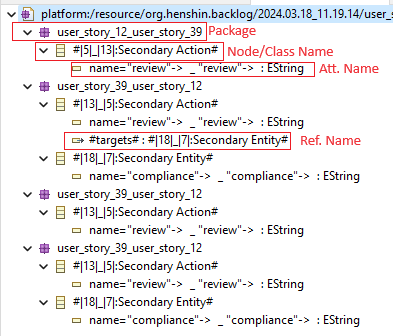
\includegraphics[scale=0.5]{minimal_model_packages}
	\caption{Representation of redundant attributes and references in \textit{minimal-model.ecore} file}\label{fig:minimal_model_packages}
\end{figure}
\begin{example}
	To illustrate this step, we also pass the transformation rules created in step 2, which reflect three USs (user\_story\_12/39/51), to the CDA tool and selecting "conflicts" as conflict type to calculate with "fine granularity" as the depth of analysis.\\
	Once the calculation is complete, the results are listed in the "CDA" -\textgreater "Results Window" as shown in Figure \ref{fig:step_3_cda_report}. Figure \ref{fig:step3_cda_report_project_tree_view} shows how the data is saved in the project's tree view, which contains all conflict reasons and atoms together in a rule pair directory.
	\begin{figure}[h]
		\centering
		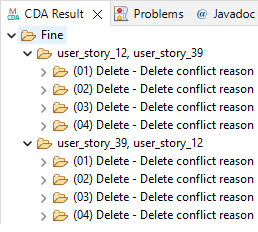
\includegraphics[scale=0.5]{step_3_cda_report}
		\caption{CDA report in relation to three transformation rules with "conflicts" as the type to be calculated and "fine granularity" as the depth of the analysis}\label{fig:step_3_cda_report}
	\end{figure}
	\begin{figure}[h]
		\centering
		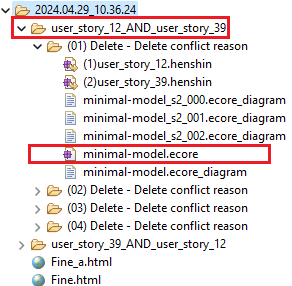
\includegraphics[scale=0.5]{step3_cda_report_project_tree_view}
		\caption{Saving CDA results data in the project's tree view}\label{fig:step3_cda_report_project_tree_view}
	\end{figure}
	As we can see, the CDA tool has only found redundancy between user\_story\_12 and user\_story\_39. This is because there are no redundant clauses between two USs (user\_story\_12 and user\_story\_39) and user\_story\_51.\\
	Regarding the redundant elements specifically, we can refer to the created file "minimal-model.ecore", which is located in the tree view of the project under each conflict reason. Figure \ref{fig:step3_cda_report_project_tree_view} show the minimal-model.ecore file related to user\_story\_12 and user\_story\_39.\\\\
	The file Minimal-model.ecore, which refers to user\_story\_12 and user\_story\_39, is divided into packages, with each package containing different matches of redundant elements. If there is a redundancy between two elements, this is explicitly indicated by a hash symbol (\#). Figure \ref{fig:step3_cda_package} illustrates the redundant elements found in each package.\\\\
	\begin{figure}[h]
		\centering
		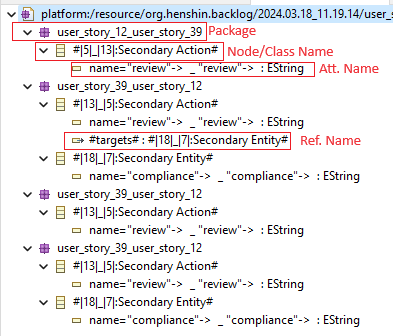
\includegraphics[scale=0.5]{minimal_model_packages}
		\caption{Representation of the redundant elements in each package within \textit{minimal-model.ecore} file}\label{fig:step3_cda_package}
	\end{figure}
	For example, the attribute "name" with the value "review" in "Secondary Action" and the attribute "targets" with the value "compliance" in "Secondary Entity" are labelled as redundant (both with a hash symbol). The reference to "targets" is also marked as redundant (with a hash symbol), which means that the reference (targets) from "Secondary Action" to "Secondary Entity" is also redundant between USs, which is a very important criterion for finding redundancy correctly.
\end{example}
\subsubsection*{Step 4: Report Extraction}\label{step_4}
To create a lightweight report for the group or individual in question, we need to extract the key information from the CDA report, e.g. redundancy US-pair, redundancy clauses, count of redundancy clauses in each part of the US (main or benefit part), and create a report as a text file with the following information:
\begin{itemize}
	
	\item A table of potential redundant pairs with the number of total redundancy clauses.
	
	\item Founded potential redundant US-pairs.
	
	\item Redundancy words and clauses of founded US-pairs. Clauses consisting of two words that have one of the relationships triggers, targets or contains.
	
	\item Text of US-pairs whose redundancy words are marked with a hash symbol (\#).
	
	\item Parts of the sentence in which words and clauses are found.
\end{itemize}
\subsubsection*{Structure of a US}
The delineation and checking of redundancy clauses within USs requires a methodical approach, especially when distinguishing between the main and the benefit part of a US-pair. This distinction is crucial to ensure that redundancy identifications within one part are not mistakenly transferred to the other. Consequently, the analytical framework comprises three conditions, each of which specifies its own methodology for case processing:
\begin{itemize}
	\item Presence of benefit in both USs of the redundancy-pair: if a benefit is identifiable in each US of the pair, a process of separation is used to split the main content from the benefit parts. After this separation, a targeted search for redundancy clauses is carried out only within the main part, whereby identified redundancies are annotated with a hash symbol (\#). This process is repeated for the benefit parts to ensure a thorough check and marking of redundancies within each individual part.
	
	\item Exclusive presence of a benefit in one US of the redundancy-pair: In scenarios where only one US of the pair contains a benefit part, the analysis is limited to the main part of both USs. The aim remains the identification and annotation of redundancy clauses within this part. The lone benefit part remains in its original state and is excluded from the redundancy check.
	
	\item Absence of benefit parts in both USs of the pair: If neither of the two USs of the redundancy-pair contains a benefit part, the focus shifts completely to the main parts. The investigation is designed to highlight redundancy clauses within these parts, whereby the benefit parts are not taken into account due to their non-existence.
	
\end{itemize}
This structured and segmented approach ensures precise and efficient identification of redundancy clauses within the USs, optimising the clarity and effectiveness of textual report.
\begin{example}
	After the CDA directory for user\_story\_12 and user\_story\_39 is created by CDA tool graphic interface (UI), we pass the location of directory into ReportExtractor class and in order to extracting the important information and save it into the texual report as well as JSON report.
	Listing \ref{list:textual_report_sample} illustrates the example of the textual report. In this case, the report only contains one US-pair.
	\begin{MyListing}
		\paragraph{}
		\centering
		%\lstinputlisting[basicstyle=\ttfamily\footnotesize]{Listing/TextualReportSample.txt}
		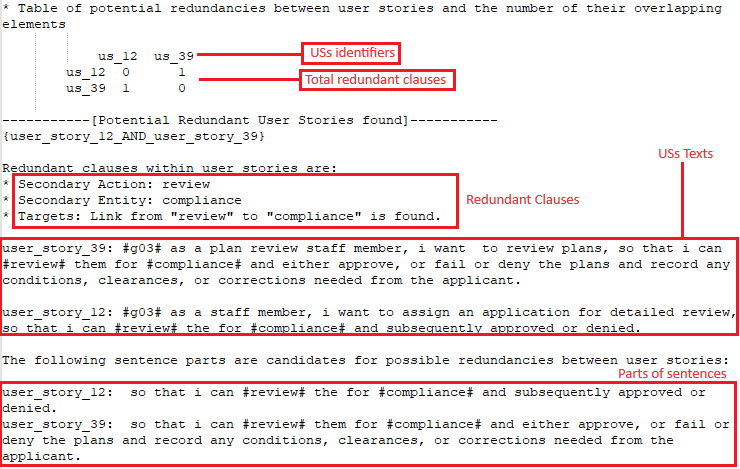
\includegraphics[scale=0.7]{Listing/TextualReportSample.png}
		\caption{Example of generated textual report for one US-pair}\label{list:textual_report_sample}
	\end{MyListing}	
	As we can see, the text report consists of a 2 x 2 table whose first column and first row are US identifiers, and the numbers inside the table are the total number (benefit part + main part) of redundancy elements between two USs; secondly, the redundant clauses related to the redundant US-pair are listed; thirdly, the text of US whose redundant phrases are marked with a hash symbol; finally, the part of the clauses in which redundant elements occur is displayed.	
\end{example}
For further evaluation purposes and easy export of the report to another platform such as Excel, a JSON report is created that collects the information about redundant US-pairs separately in a JSON object with the following entries:
\begin{itemize}
	\item Potential Redundant User Stories:  which has stored the US-pair identifier(e.g. "user\_story\_12\_AND\_user\_story\_39"). 
	
	\item Status: consisting of "Main/Beneift Part Redundancy Clauses" and "Total Redundancy Clauses", which store the count of redundancy clauses in the main and benefit part as well as in the total part of the US.
	
	\item Entity: which can consist of a "Secondary/Primary Entity" and stores the founded redundant entities.
	
	\item Common Targets/Contains: which consists of the "Main Part" and "Benefit Part" entries and only stores the targets/contains relationships that are common between the USs in a particular part of the USs. For example, if there are common redundant targets in the main part of the USs, these are included in the "Main Part" entity of the "Common Targets".
	
	\item Text: consisting of two entries, namely "First UserStory" and "Second UserStory", in which the text of the US-pair whose hash symbol has already been applied in redundant phrases is stored.
	
	\item Project Number: stores the number of the Project(e.g. "G03").
	
	\item Part of Sentence: consists of the entries "First UserStory" and "Second UserStory", in which the part of the US sentences containing redundant clauses is stored.
	
	\item All Targets/Contains: which consists of the "Main Part" and "Benefit Part" entries and stores the whole targets/contains relationships that are occurred in the particular part of the USs.
	
\end{itemize}
\begin{example}
	Listing \ref{list:json_report_sample} illustrates the example of the JSON report regarding user\_story\_12 and user\_story\_39.
\end{example}
\begin{MyListing}
	%\paragraph{}
	
	\centering
	%\lstinputlisting[basicstyle=\ttfamily\footnotesize]{Listing/TextualReportSample.txt}
	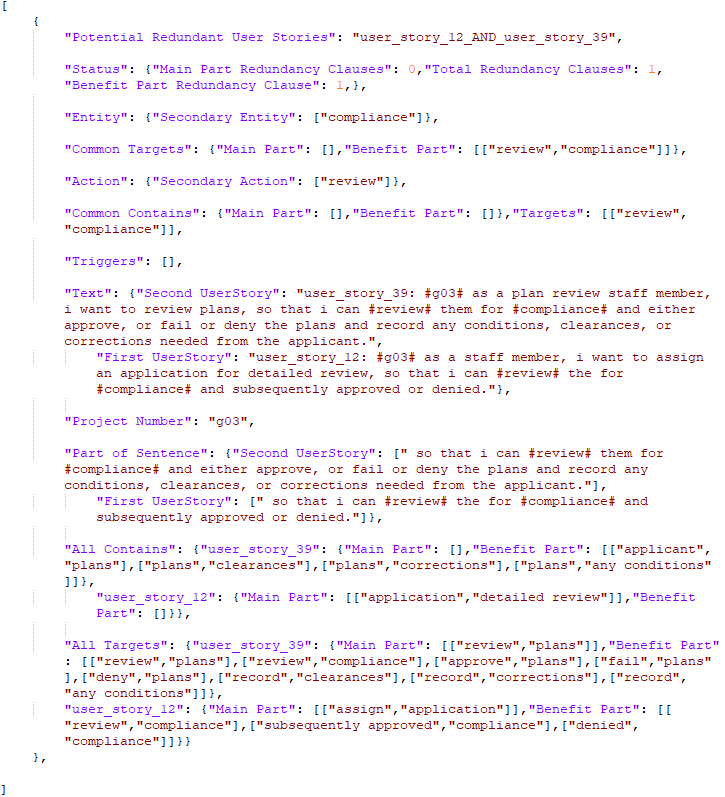
\includegraphics[scale=0.7]{Listing/JSONReportSample.png}
	\caption{Example of generated JSON report for one US-pair}\label{list:json_report_sample}
	
\end{MyListing}	
\subsubsection*{Step 5: Report Evaluation}
The Evaluation class, part of the \textit{org.henshin.backlog.code.evaluation} package, was developed to determine the level of redundancy in USs based on JSON reports. This class provides methods to evaluate whether two USs are either fully or partially redundant, analysing different application components of these USs.

The evaluation process involves a complex logic to determine whether USs are redundant. This includes:
\begin{itemize}
	\item Checking whether the arrays are empty or contain similar elements.
	\item Comparing the individual elements in the arrays for both USs to determine if they fully match (full redundancy) or if they have some common elements (partial redundancy).
\end{itemize}
\begin{example}
	For the two US-pairs of dataset G03, we apply the evaluation class to determine whether there is redundancy in the main or benefit part, and if so, what type of redundancy is recognised(full or partially).\\\\
	As shown in Listing \ref{list:json_evaluation}, four entries are added to the JSON report, namely "Main Partially Redundant", "Benefit Part Fully Redundant",
	"Main Part Fully Redundant", "Benefit Partially Redundant" as "Status" which their value is whether true or false. 
	\begin{MyListing}
		\paragraph{}
		
		\centering
		%\lstinputlisting[basicstyle=\ttfamily\footnotesize]{Listing/TextualReportSample.txt}
		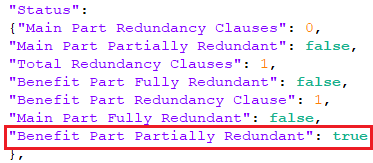
\includegraphics[scale=0.7]{Listing/json_evaluation.png}
		\caption{Example of generated entries in JSON report regarding evaluation of level of redundancy in main or benefit part}\label{list:json_evaluation}
		
	\end{MyListing}	
	
	In the case of user\_story\_12 and user\_story\_39, the entry "Benefit Partially Redundant" was marked as \textit{true}, which means that US-pair in benefit parts are partially redundant.
	
\end{example}
The class performs these checks by iterating through the JSON arrays of Triggers, Targets and Contains and comparing each element with those in the common sections to determine redundancy.


\subsection{Implementation}\label{redundancy_implementation}
In this section, we explain the objective and scope of the implementation, the functionality and the programming languages used.

The entire implementation is available in the GitHub repository \footnote{\href{https://github.com/amirrabieyannejad/Redundancy_Analysis/tree/main}{https://github.com/amirrabieyannejad/Redundancy\_Analysis/tree/main}}.
%\subsubsection*{Objective and Scope}
%The goal and scope of the work is divided into four phases. Firstly, converting the USs annotated by the CRF tool into graph transformation rules; secondly, using the CDA tool of the Henshin to automatically report redundancies between USs pairwise; thirdly, extracting important information from the CDA report into a text report; fifthly, evaluation of reports. %For further analysis, we stored the information in a JSON file to be able to import the data into another platform such as Excel.
%Figure \ref{fig:implementation_phases} illustrates the mentioned implementation phases.
%\begin{figure}[h]
%	\centering
%	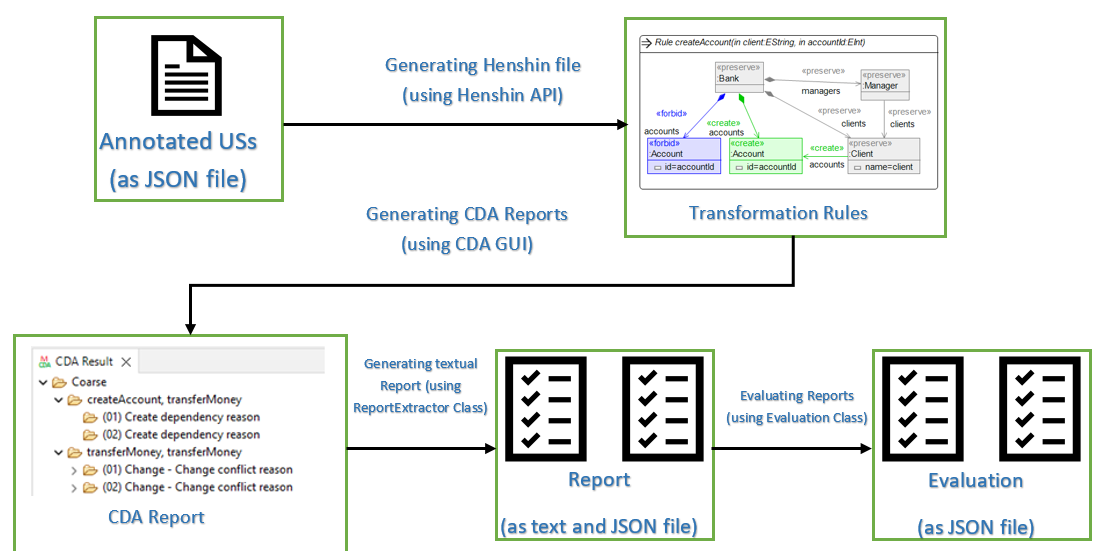
\includegraphics[scale=0.3]{implementation_phases}
%	%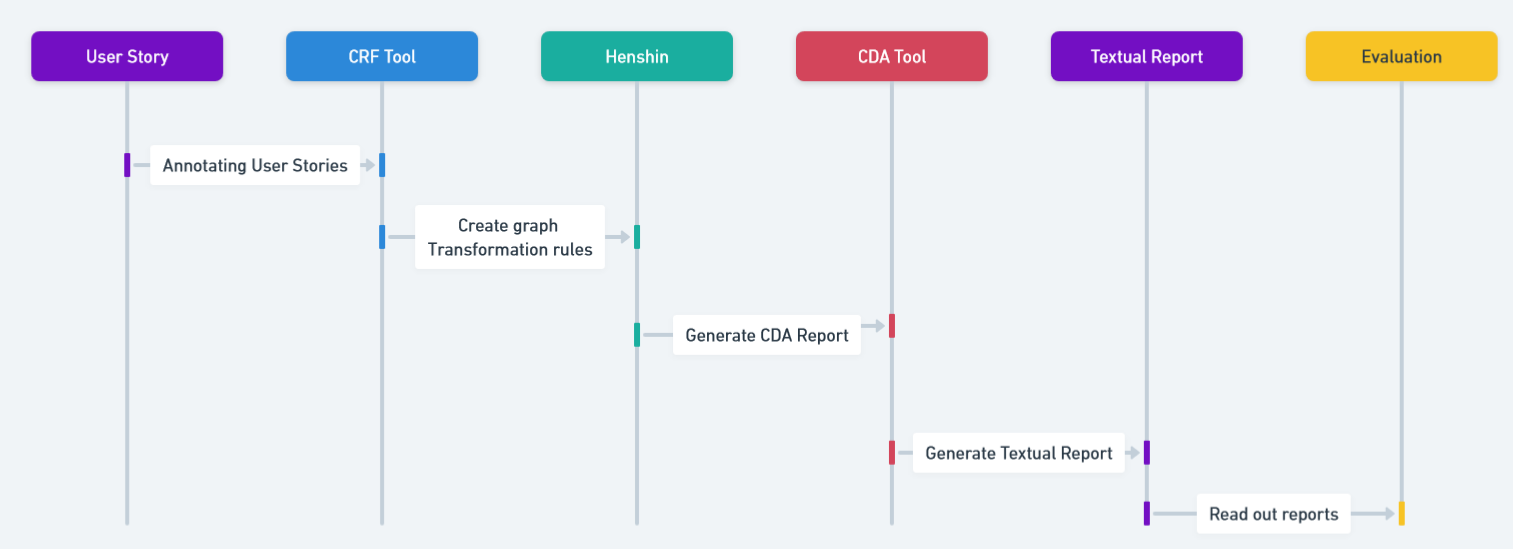
\includegraphics[scale=0.35]{sequence_diagram}
%	\caption{Three Implementation phases}\label{fig:implementation_phases}
%\end{figure} 
\subsubsection*{Methodology}
This section explains and introduces tools that are required during the development process.

Following approach and tools are necessary in order to develop our workflow:
\begin{itemize}	
	\item Java as programming language\footnote{\href{https://www.java.com/de/}{https://www.java.com/de/}}: Java is a widely used object-oriented programming language and software platform that is used to implement the Henshin and EMF APIs, which are critical to our approach to utilising them. Therefore, we use Java as our programming language.
	
	\item GitHub as version control\footnote{\href{https://github.com/}{https://github.com/}}: GitHub is a developer platform that allows developers to create, store, manage and share their code. It uses Git software, providing the distributed version control of Git plus access control, bug tracking, software feature requests, task management, continuous integration, and wikis for every project.
\end{itemize} 
\subsubsection*{Implementation Phases}\label{implementation_phases}
This section contains a step-by-step guide to implementation, starting with the set-up and ending with the final evaluation.
%\subsubsection*{Step 1: Data Preparation}\label{step_1}
%As primary input, we receive a graph-based model generated by the CRF tool, which represents the refined and annotated dataset for the recognition of \emph{entities}, \emph{actions}, \emph{persons} and \emph{benefits} of USs \cite{mosser2022modelling}.
%The datasets have the JSON format, the structure of which is very important in the Java classes \textit{RuleCreator}, \textit{ReportExtractor}, and \textit{Evaluation}. Therefore, understanding the JSON format provided is needed for the further procedure.
%Each JSON file for a backlog dataset contains a JSON-array in which each US entry is defined as a JSON-object. Listing \ref{list:json_format} illustrates the format used for the US entry.
%\begin{MyListing}
%	\paragraph{}
%	\hrule
%	\centering
%	\lstinputlisting[basicstyle=\ttfamily\footnotesize]{Listing/json_format.json}
%	\caption{The JSON format of each US entry in JSON file}\label{list:json_format}
%	\hrule
%\end{MyListing}
%Mooser et al. have linked each \emph{Persona} to each \emph{Primary Action} as \emph{Trigger} relationships, each \emph{Primary Actions} to each \emph{Primary Entity} as \emph{Target} relationships and each \emph{Primary/Secondary Entity} to each \emph{Primary/Secondary Entity} implying a \emph{Contains} relationship\cite{arulmohan2023extracting}.
%To interact with the entries in JSON file, we need to distinguish between the entries that are defined as JSON-objects, such as: {Text, Action, Entity, Benefit, US\_Nr} and the entries that are defined as a JSON-array, such as: {Persona, Primary/Secondary Action, Primary/Secondary Entity, Triggers, Targets, Contains}.
%In order to parsing JSON file, we use \enquote{org.json} library which provide us the classes as follow:
%\begin{itemize}
%	\item \enquote{JSONObject}: An unordered collection of key and value pairs.
%	\item \enquote{JSONArray}: Provide an ordered sequence of values.
%	\item \enquote{JSONTokener}: A tool that breaks a piece of text into a series of tokens that can be used by JSONObject or JSONArray to parse JSON entries.
%\end{itemize}
%\subsubsection*{Identifying USs in JSON-File}\label{workflow_nummerize_us}
%Annotated USs in each JSON file have no identifier. To distinguish USs, we use a Python script called \textit{nummerise\_us.py} \footnote{https://github.com/amirrabieyannejad/USs\_Annotation/tree/main/Script/numberise\_us}, which receives JSON files as input and adds a JSON object named \enquote{US\_Nr} with an identifier as value (e.g. user\_story\_01) to each US and returns the JSON files as output.
%Listing \ref{list:json_format_sample} illustrates the added JSON object "US\_Nr" and its value in the JSON file.
%\begin{MyListing}
%	\paragraph{}
%	\hrule
%	\centering
%	\lstinputlisting[basicstyle=\ttfamily\footnotesize]{Listing/json_format_sample.json}
%	\caption{The JSON format with the additional JSON object "US\_Nr" and its value}\label{list:json_format_sample}
%	\hrule
%\end{MyListing}
\subsubsection*{Creation of Rules}\label{step_creation_of_ruels}
In this section, we explain the methods we used to convert the US data structured in JSON files into transformation rules using the Henshin API. The process starts with the creation of an Ecore meta model, as explained in Section \ref{design_step_2}, which reflects the structure of the data. The Henshin transformation rules are then generated using the RuleCreator class and its methods.
%\subsubsection*{Data Structures}
%The datasets of the backlogs annotated with the CRF tool have the JSON format, the structure of which is very important in the Java classes \textit{RuleCreator} and \textit{ReportExtractor}. Therefore, understanding the JSON format provided is crucial for the further procedure.

%Each JSON file for a backlog dataset contains a JSON-array in which each US entry is defined as a JOSN-object. Listing \ref{list:json_format} illustrates the format used for the US entry.
%\begin{MyListing}
	%\paragraph{}
	%\hrule
	%\centering
	%\lstinputlisting[basicstyle=\ttfamily\footnotesize]{Listing/json_format.json}
	%\caption{The JSON format of each US entry in JSON file}\label{list:json_format}
	%\hrule
%\end{MyListing}
%To interact with the entries in JSON file, we need to distinguish between the entries that are defined as JSON-objects, such as: {Text, Action, Entity, Benefit, US\_Nr} and the entries that are defined as a JSON-array, such as: {Persona, Primary/Secondary Action, Primary/Secondary Entity, Triggers, Targets, Contains}.
%In order to parsing JSON file, we use \enquote{org.json} library which provide us the classes as follow:
%\begin{itemize}
	%\item \enquote{JSONObject}: An unordered collection of key and value %pairs.
	%\item \enquote{JSONArray}: Provide an ordered sequence of values.
%	 \item \enquote{JSONTokener}: A tool that breaks a piece of text into a series of tokens that can be used by JSONObject or JSONArray to parse JSON entries.
%\end{itemize}
%Provide detailed explanations of key implementation aspects, such as algorithms, data structures, design patterns, and any custom solutions developed. Discuss any challenges faced during implementation and how you addressed them.
\subsubsection*{Methods of the RuleCreator Class}
In this section, the methods of the RuleCreator class is described as follows:
\begin{itemize}
	
	\item AssignCmodule: This method assign a CModule to a Ecore meta-model. It creates a new CModule object with the provided Henshin-file name, adds imports from the Ecore file, and returns the module.
	
	\item processJsonFile: It takes parsed JSON array as input and processes their attributes, such as persona, actions, entities, text and their edges, such as targets, triggers. Corresponding elements are created as output in a the Henshin transformation module (CModule).
	
	\item processRule: It takes the \enquote{US\_Nr} JSON-object as input and creates a new CRule with the name of unique US identifier in the CModule.
	
	\item processPersona: It receives as input the persona extracted from the JSON data and the associated CRule to create a new CNode representing the persona within the provided CRule and adds the attribute \enquote{name} with persona as value. Finally, the created CNode representing the persona is returned.
	
	\item processText: It receives as input US text extracted from JSON data and the associated CRule to create a new CNode representing the text within the provided CRule and adds the attribute \enquote{text} with US text as value. Finally, the created CNode representing the US text is returned.
	
	\item processActions: The processActions method is responsible for creating CNode objects that represent actions within the CModule. As parameters, it receives the JSON-object of the actions, the CNode-object representing the persona associated with the actions and the unique identifier of the US. Since the edge triggers only refer to the persona and the primary action, a new CNode is created for each primary action that represents the primary action within the provided CRule, an attribute \enquote{name} is added and an edge is created from the persona node to the primary action with the label \enquote{triggers}. For each secondary action, a new CNode is created to represent the action within the provided CRule and an attribute \enquote{name} is added to the action node.
	
	\item checkEntityIsTarget: It receives the name of the entity and the JSON-array with information about targets edges. The method iterates through the JSON-array targets, which contains arrays that represent targets edges between actions and entities. It compares the targets entity with the specified entity. If there is a match, true is returned to indicate that the entity belongs to a targets relation.
	
	\item processEntities: It receives as parameters the JSON-object with information about the entities, the CRule object representing the US to which the entities belong and the JSON-array with information about the targets associated with the entities. The method checks whether primary/secondary entities are present, then creates a CNode for each primary/secondary entity and checks whether the entity is present in the targets array. If this is the case, its attribute \enquote{name} is annotated for deletion. This method is used within the \textit{processContainsEdges} method to determine whether an entity involved in a contains relation is also a targets of another entity.
	
	\item processContainsEdges: It receives the JSON-object to be processed, the JSON array with information about contains/targets edges and the US identifier as parameters. It first checks whether both entities belong to contains edges. If both entities exist, an edge is created between them in CRule with the label \enquote{contains}. If one of the entities is a targets of another entity (as specified in the targets array), the edge is annotated as \textit{delete}. If none of the entities is a targets, the edge is annotated as \textit{preserve}.
	
\end{itemize}
Figure \ref{fig:rule_creator_class_diagram} is a class diagram that illustrates the attributes, operations and relationships related to the RuleCreator class.
\begin{figure}[h]
	\centering
	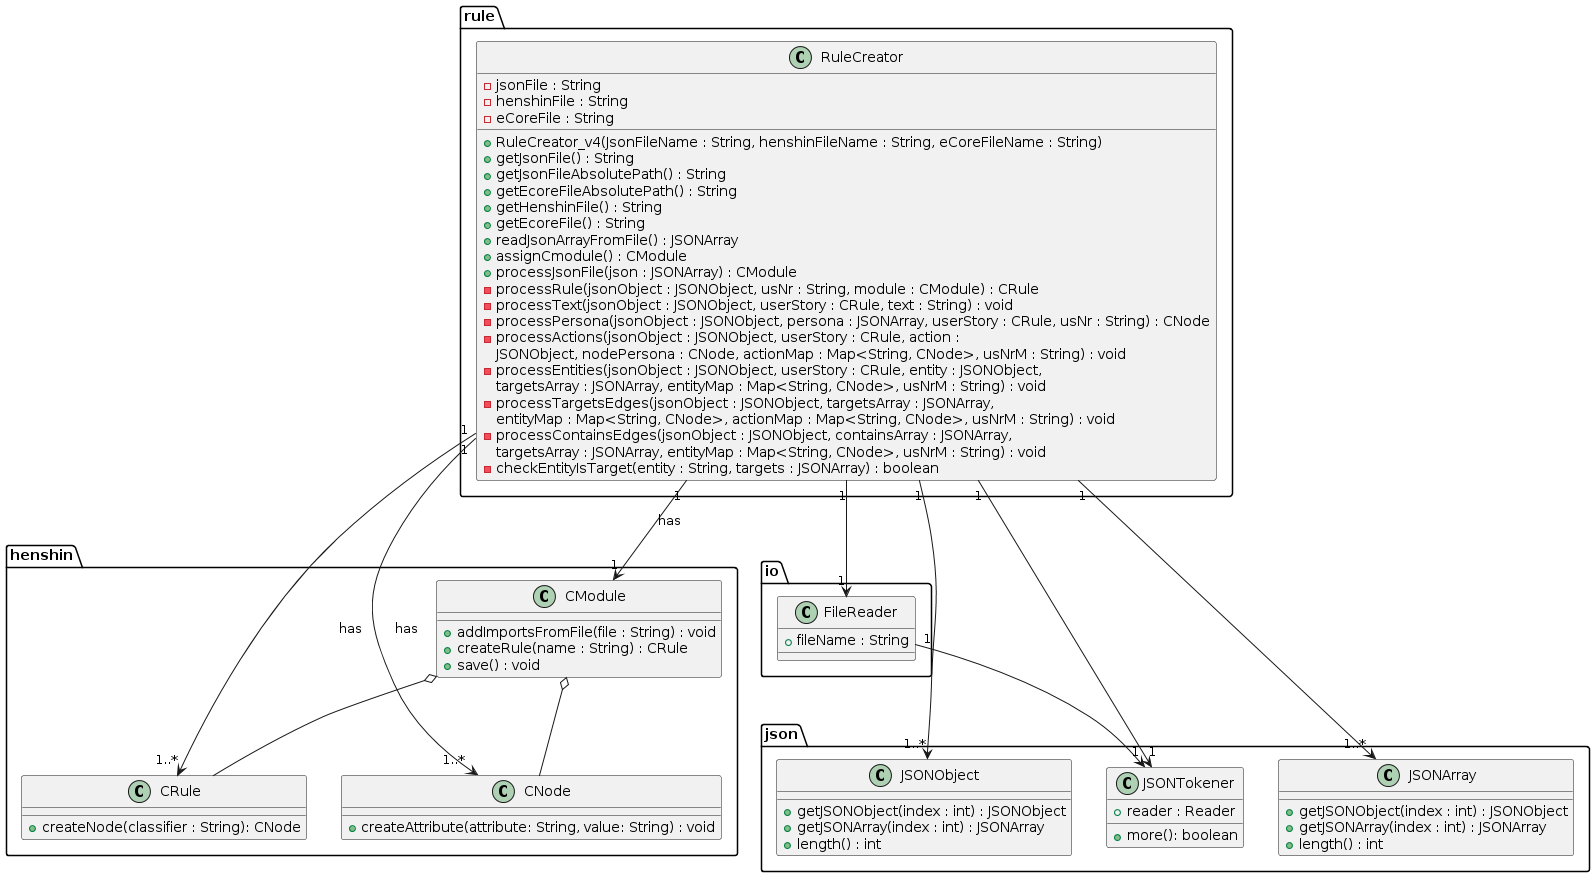
\includegraphics[scale=0.3]{rule_creator_class_diagram}
	\caption{Class diagram of the RuleCreator class and its relationships}\label{fig:rule_creator_class_diagram}
\end{figure}
%To illustrate this step, three example is given in which the RuleCreator class is applied to a dataset (G03) with three collected USs and the resulting artefact is presented.
%\begin{example}
%Listing \ref{list:json_user_story_12} shows the JSON format in relation to user\_story\_12 and Figure \ref{fig:rule_user_story_12} shows the application of the RuleCreator class in this US, which is a transformation rule where the targets and the associated contains relationships are annotated as a \textless Delete\textgreater action and the rest of the nodes and edges are annotated as a \textless Preserve\textgreater action.\\\\
%Text of US is:
%user\_story\_12: "\#G03\# As a Staff member, I want to Assign an Application for Detailed Review, so that I can review the for compliance and subsequently approved or denied."
%Considering the backlog dataset as shown in Listing \ref{list:backlog_g03}:
%\begin{MyListing}
%	\paragraph{}
%	\centering
%	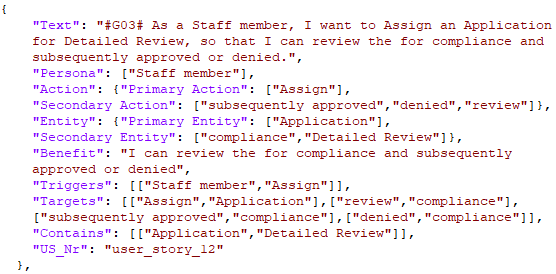
\includegraphics[scale=0.8]{Listing/json_user_story_12.png}
%	\caption{JSON entities Related to %user\_story\_12}\label{list:json_user_story_12}
%\end{MyListing}
%\begin{figure}[h]
%	\centering
%	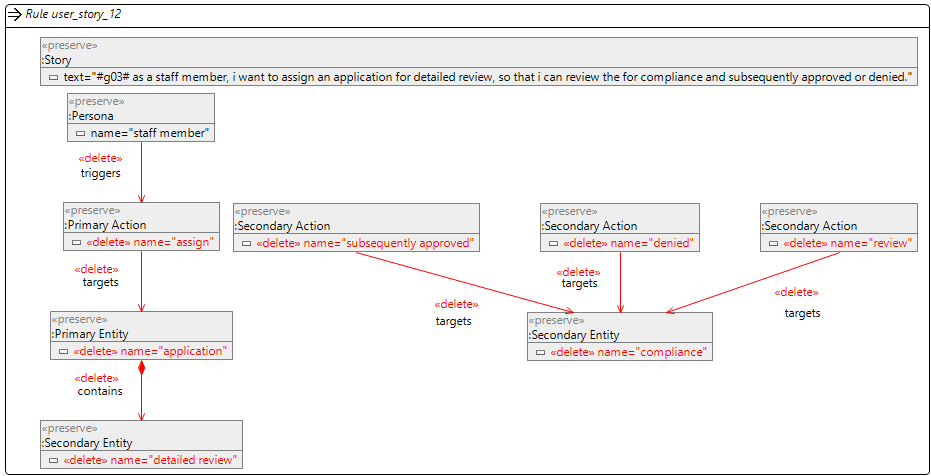
\includegraphics[scale=0.6]{rule_user_story_12}
%	\caption{Generated transformation rule related to user\_story\_12 using RuleCreator class}\label{fig:rule_user_story_12}
%\end{figure}
%As we can see, the "targets" edges and their direct relationships ("triggers" and "contain", if any) are also annotated as \textless delete\textgreater, which is very important to find redundant elements with the CDA tool.
%\end{example}
%\begin{example}
%Listing \ref{list:json_user_story_39} shows the JSON entities related to user\_story\_39 and Figure \ref{fig:rule_user_story_39} shows transformation rule generated by RuleCreator class.\\\\
%Text of US is:
%user\_story\_39: "\#G03\# As a Plan Review Staff member, I want to Review Plans, so that I can review them for compliance and either approve, or fail or deny the plans and record any conditions, clearances, or corrections needed from the Applicant."
%\begin{MyListing}
%	\paragraph{}
%	\centering
%	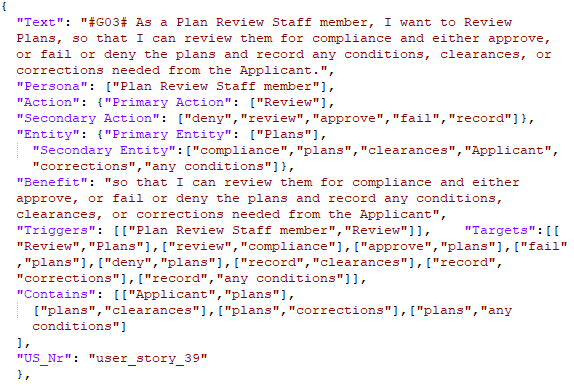
\includegraphics[scale=0.8]{Listing/json_user_story_39.png}
%	\caption{JSON entities Related to user\_story\_39}\label{list:json_user_story_39}
%\end{MyListing}
%\begin{figure}[h]
%	\centering
%	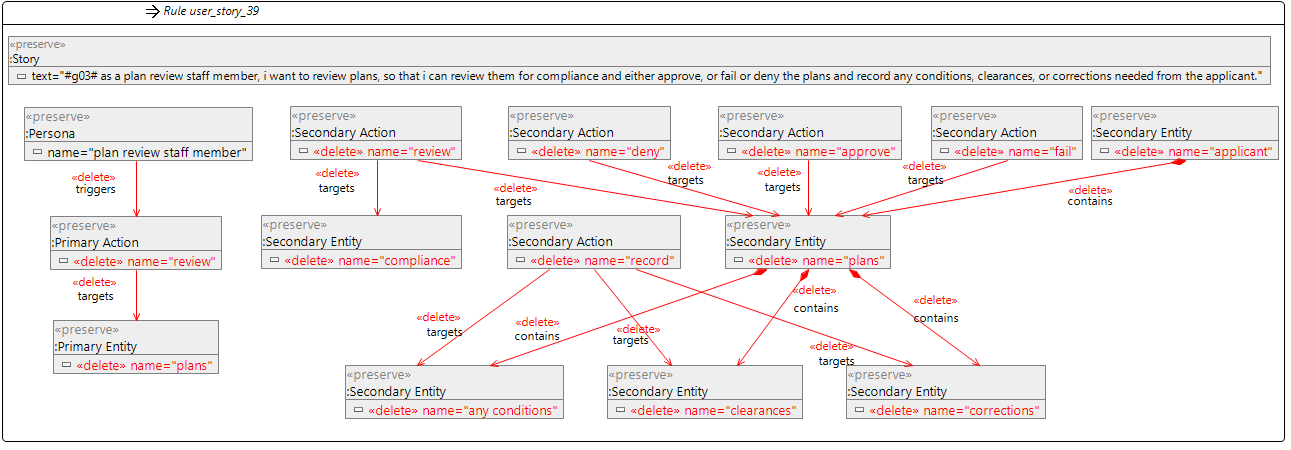
\includegraphics[scale=0.43]{rule_user_story_39}
%	\caption{Generated transformation rule related to user\_story\_39 using RuleCreator class}\label{fig:rule_user_story_39}
%\end{figure}
%Attribute "Plan", as we can see, it appears both in the main part as a primary entity and in the benefit part as a secondary entity, forming the various relationships as targets and contains.
%\end{example}

%\begin{example}
%Listing \ref{list:json_user_story_51} shows the JSON entities related to user\_story\_51 and Figure \ref{fig:rule_user_story_51} shows transformation rule generated by RuleCreator class.\\\\
%Text of US is:
%user\_story\_51: "\#G03\# As an Enforcement Staff member, I want to Issue a Notice of Violation, so that I can provide formal communication to the responsible party."
%\begin{MyListing}
%	\paragraph{}
%	\centering
%	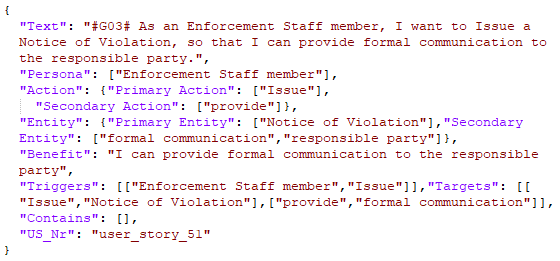
\includegraphics[scale=0.8]{Listing/json_user_story_51.png}
%	\caption{JSON entities Related to user\_story\_51}\label{list:json_user_story_51}
%\end{MyListing}
%\begin{figure}[h]
%	\centering
%	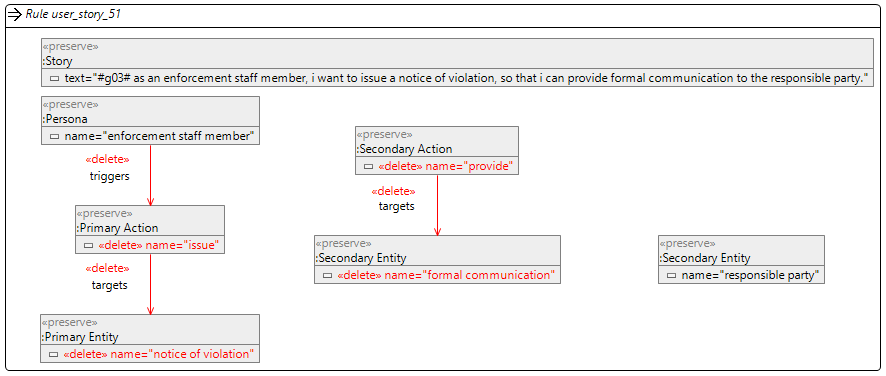
\includegraphics[scale=0.55]{rule_user_story_51}
%	\caption{Generated transformation rule related to user\_story\_51 using RuleCreator class}\label{fig:rule_user_story_51}
%\end{figure}
%Last but not least, we have determined that the secondary entity "responsible party" has neither a target nor a contains relationship. Therefore, it is not annotated as \textless delete\textgreater, but as \textless preserve\textgreater. This is due to the fact that some phrases have been identified as entities in the CRF tool, but their relationship is not annotated at all, which is problematic for analysing redundancy.
%\end{example}
\subsubsection*{Report Extraction}\label{step_report_extraction}
In order to extracting a textual report associated with a specific backlog, we implement a class called \textit{ReportExtractor} within the package \textit{org.henshin.backlog.code.report}, which include the following classes from the package \textit{org.eclipse.emf.ecore}\footnote{\href{https://download.eclipse.org/modeling/emf/emf/javadoc/2.7.0/org/eclipse/emf/ecore/}{https://download.eclipse.org/modeling/emf/emf/javadoc/2.7.0/org/eclipse/emf/ecore/}}. These classes are important for reading the content of \textit{minimal-model.ecore}:
\begin{itemize}
	
	\item org.eclipse.emf.ecore.resource.Resource: A resource of an appropriate type is created by a resource factory; a resource set indirectly creates a resource using such a factory. A resource is typically contained by a resource set, along with related resources.
	
	\item org.eclipse.emf.ecore.resource.ResourceSet: A resource set manages a collection of related resources and notifies about changes to this collection. It provides a tree of content. A collection of adapter factories supports the search for an adapter via a registered adapter factory. 
	
	\item org.eclipse.emf.ecore.EObject: EObject is the root of all modelled objects, therefore all method names start with "E" to distinguish the EMF methods from the client methods. It provides support for the behaviour and functions that are common to all modelled objects.
	
	\item org.eclipse.emf.ecore.EPackage: A representation of the model object \enquote{EPackage}.
	
	\item org.eclipse.emf.ecore.EClassifier: A representation of the model object \enquote{EClassifier}.
	
	\item org.eclipse.emf.ecore.EClass: A representation of the model object \enquote{EClass}.
	
	\item org.eclipse.emf.ecore.EAttribute: A representation of the model object \enquote{EAttribute}.
	
	\item org.eclipse.emf.ecore.EReference:  A representation of the model object \enquote{EReference}.
	
\end{itemize}
\subsubsection*{Storing Redundancy Items into RedundancyItems Class}
To save the redundant elements found by the CDA tool, we implement classes to save the elements according to their type.

Figure \ref{fig:redundancyItems_class_diagram} is a class diagram that illustrates the attributes, operations and relationships related to the ReundancyItems class to store the redundancy elements provided by the CDA tool.
\begin{figure}[h]
	\centering 
	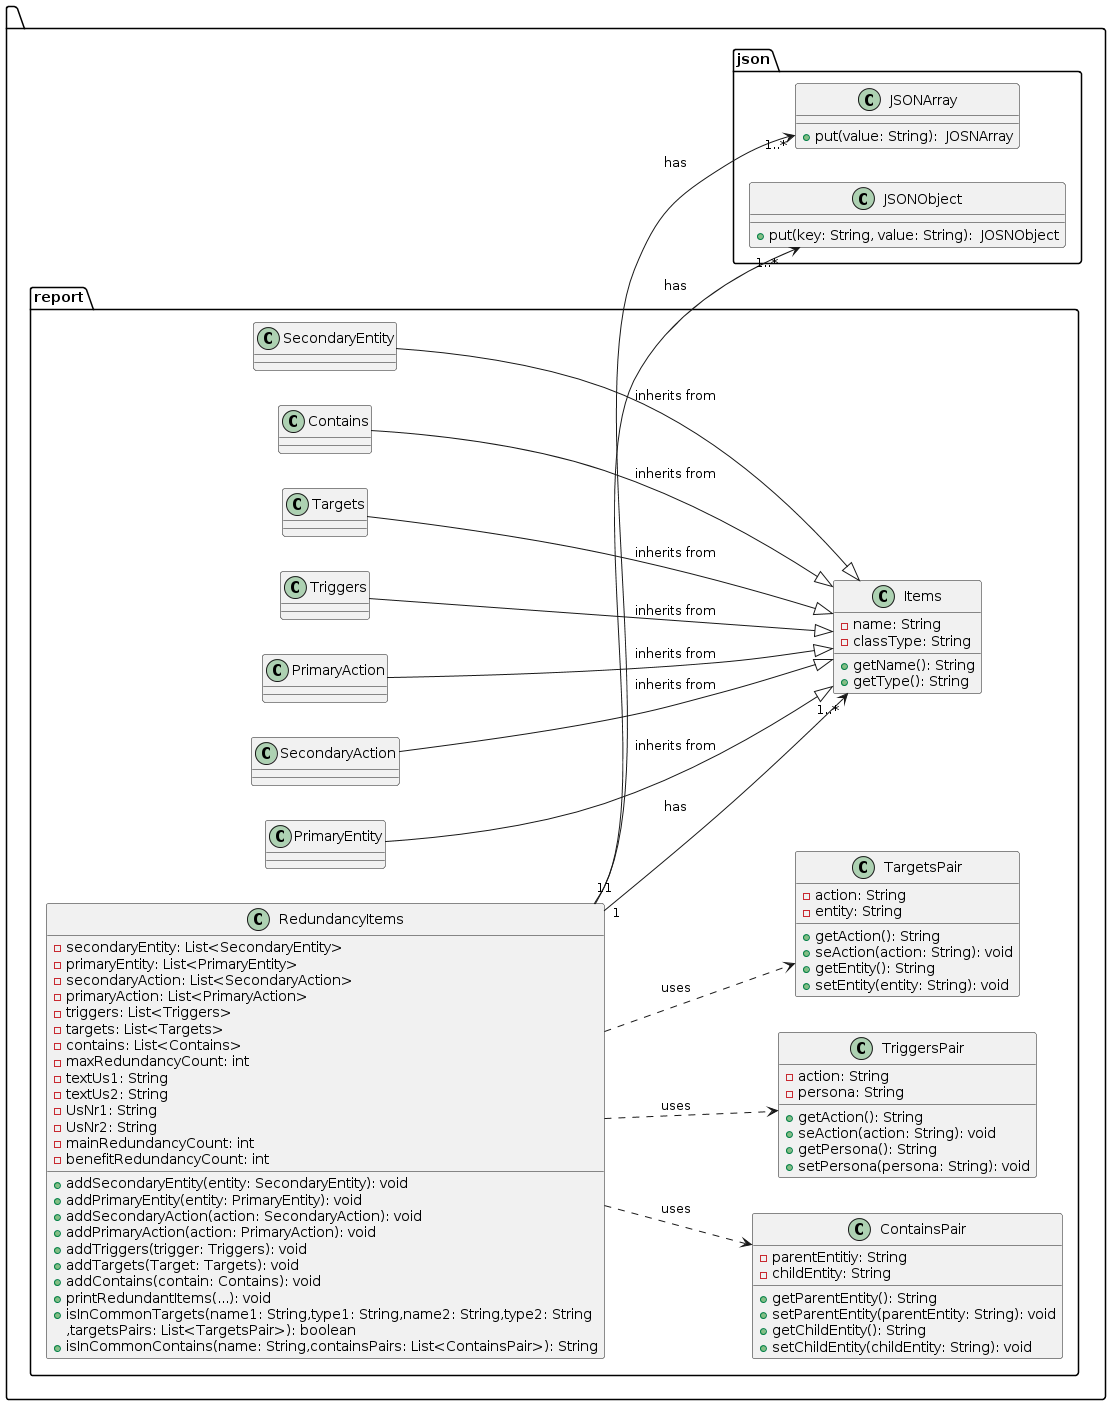
\includegraphics[scale=0.36]{redundancyItems_class_diagram.png}
	\caption{Class diagram for the RedundancyItems class and its relationship}\label{fig:redundancyItems_class_diagram}
\end{figure} 
The following classes were created to represent the extracted model object accordingly. All these classes are extensions of the class \textit{RedundancyItems}, which contains all extracted model object from \enquote{minimal-model.ecore} such as \enquote{EClass}, \enquote{EAttribute} or \enquote{EReference}:
\begin{itemize}
	
	\item PrimaryAction/SecondaryAction: Which has only saved the EClass specified by \enquote{Primary/Secondary Action} and the EAttribute model object with the methods \textit{getType} to retrieve the saved EClass and \textit{getName} to retrieve the saved EAttribute.
	
	\item PrimaryEntity/SecondaryEntity: Which has only saved the EClass specified by \enquote{Primary/Secondary Entity} and the EAttribute model object with the methods \textit{getType} to retrieve the saved EClass and \textit{getName} to retrieve the saved EAttribute.
	
	\item Targets: The EClass specified by \enquote{Primary/Secondary Action} as \textit{outgoing edge} and an EAttribute model object as \textit{incoming edge} with \enquote{Primary/Secondary Entity}. The method \textit{getType} retrieve the stored EClass and method \textit{getName} retrieve the stored EAttribute.
	
	\item Contains: The EClass specified by \enquote{Primary/Secondary Entity} as \textit{outgoing edge} and an EAttribute model object as \textit{incoming edge} with \enquote{Primary/Secondary Entity}. The method \textit{getType} retrieve the stored EClass and method \textit{getName} retrieve the stored EAttribute.
	
	\item Triggers: The EClass specified by \enquote{Persona} as \textit{outgoing edge} and an EAttribute model object as \textit{incoming edge} with \enquote{Primary Action}. The method \textit{getType} retrieve the stored EClass and method \textit{getName} retrieve the stored EAttribute.
	
	\item RedundantPair: Stores the identifier of the two USs that were founded as a redundant pair. It also stored the total count of redundancy clauses of US-pair.
	
	\item TargetsPair: Stores effective value of \enquote{\textit{Primary/Secondary Action}} and \enquote{\textit{Primary/Secondary Entity}} in action and entity fields accordingly.
	
	\item ContainsPair: Stores effective value of \enquote{\textit{Primary/Secondary Entity}} as \enquote{\textit{parent/child entity}} due to the fact that parent entity is a containment of child entity.
	
	\item TriggersPair: Stores effective value of \enquote{\textit{Persona}} as a persona and \enquote{\textit{Primary Action}} as an action.
	
\end{itemize}
The class RedundancyItems contains following methods which are important for class ReportExtractor:
\begin{itemize}
	\item isInCommonContains: This method is designed to determine whether a given entity (specified by its name) is part of a redundant pair listed in the \enquote{Contains} array of related USs stored in a JSON file.
	
	As input, it receives the name of the entity for which we want to check whether it exists in a redundant pair. In addition, a list of redundant pair objects that represent pairs of entities where one entity contains the other. If there is a match with the parent entity, it returns the child entity and vice versa.
	\item isInCommonTargets: This method is responsible for determining whether a particular action/entity is part of a redundant pair listed in the "Targets" array of related USs stored in a JSON file.
	
	As input, it receives the name and type of the first element, which is an action, and the name and type of the second element, which is an entity. It also receives a list of TargetsPair objects, which are pairs of common actions and entities between US-pairs.
	
	For each pair, it checks whether the specified names and types match either the action or entity in the pair. If a match is found, the method returns \textit{true}, which means that the specified elements are part of a redundant pair.
	\item printRedundantItems: This method is responsible for creating a report on redundancy items based on the data stored in the class instance. 
	
	As input, it takes several parameters, including a "FileWriter" to write to the textual report's file, lists of different pairs of "Targets", "Contains" and "Triggers", and a JSON-object to store the report data in JSON format, which is vital for evaluation process.
\end{itemize}
\subsubsection*{ReportExtractor Class: Methods related to Extracting Redundancy Items}
To extract the redundant elements and save them in a redundancyItems object, we must first iterate through all existing \textit{minimal-mode.ecore} files and extract the redundant item from each EPackage.

Figure \ref{fig:report_extractor_class_diagram} is a class diagram that illustrates the attributes, operations and relationship related to the extraction of redundancy items founded by the CDA tool and their storage in a RedundancyItems object.
\begin{figure}[h]
	\centering
	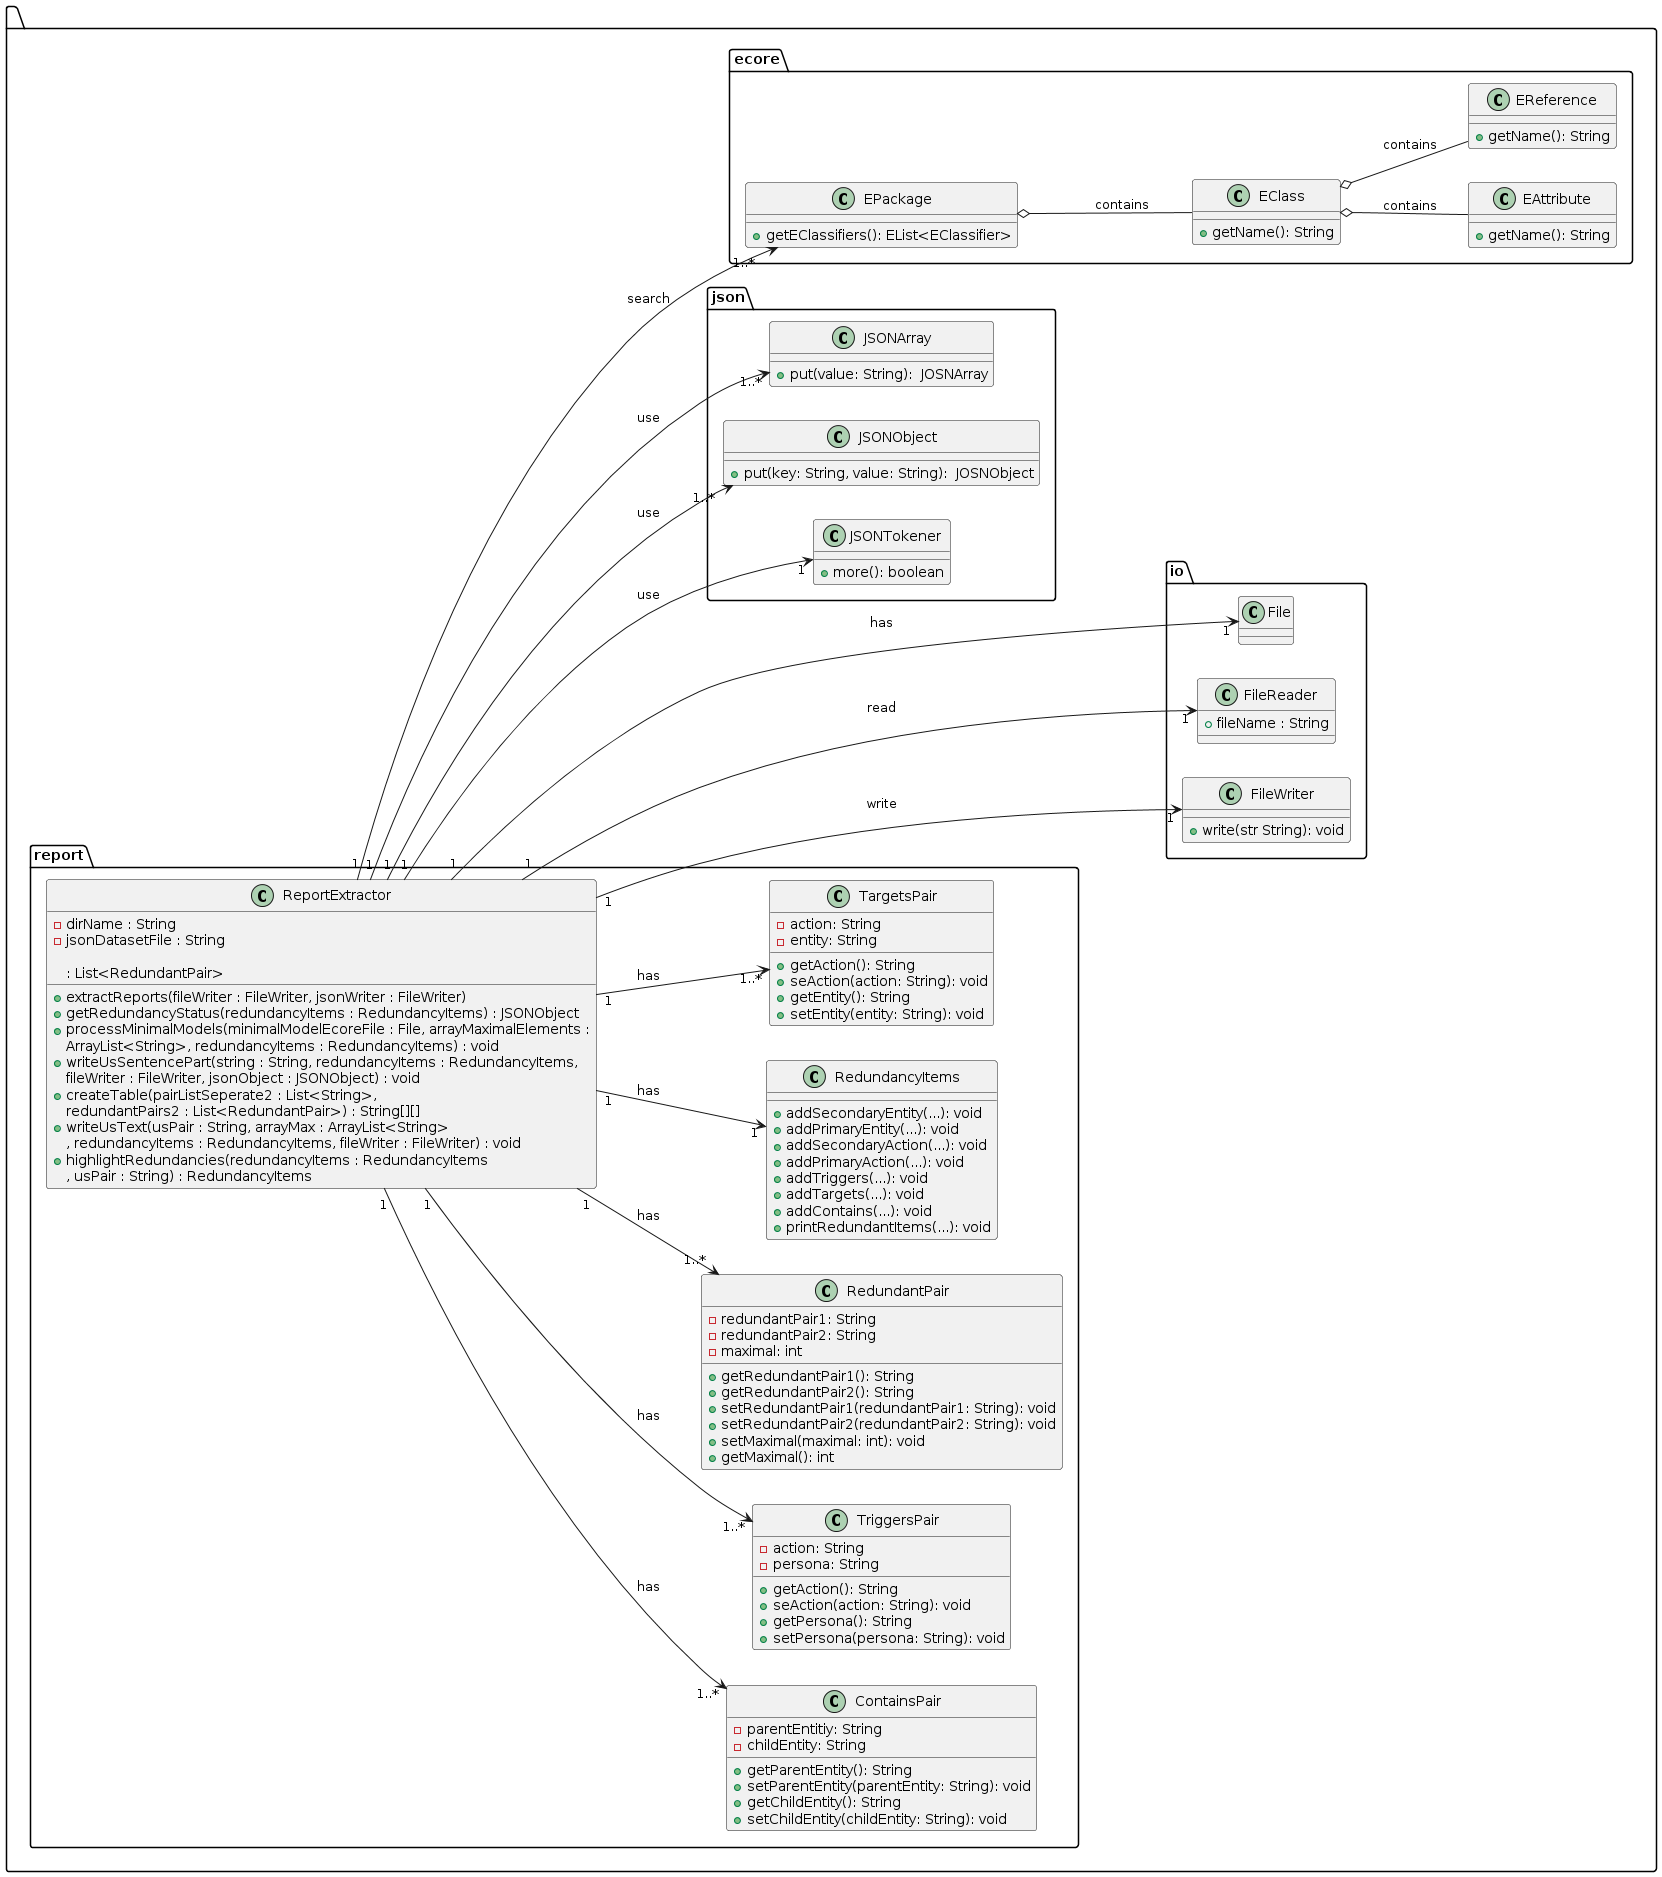
\includegraphics[scale=0.27]{report_extractor_class_diagram}
	\caption{Class diagram for the process of extracting redundancy items}\label{fig:report_extractor_class_diagram}
\end{figure} 

The following methods in the ReprortExtractor class are responsible for extracting the redundancies found by the CDA tool:
\begin{itemize}
	\item extractReports: This method orchestrates the extraction and analysis of created CDA report from a directory containing conflicted US-pairs and their associated reasons(conflict reason), and generates both text and JSON reports for further investigation and processing.
	
	It receives two fileWriter objects as input, one for writing textual and one for JSON reports.
	
	It iterates through each directory in the main directory that represents a conflict pair and uses the \textit{checkIfReportExist} method to make sure that the current US-pair are not already proceeded and the \textit{containsAnd} method to check whether it contains the conjunction \enquote{AND} to make sure that it is the valid US-pair name (\textit{e.g.} "user\_stroy\_12\_AND\_user\_stroy\_39" is a valid directory name).
	
	For each valid conflict pair directory, it iterates through the conflict reason directories within the current conflict pair directory and uses the \textit{minimalEcoreExist} method to check whether a \textit{minimal-model.ecore} file exists with reference to a conflict reason.
	
	To identify redundancy items, it uses the method \textit{processMinimalModels} and reads the "minimal-model.ecore" file, processes its content and iterates over the contained EPackages in order to process them further with the method \textit{iteratePackages}, which saves all redundancy items in a RedundacyItems object.
	
	In addition, the methods \textit{hasEntitys}, \textit{hasActions} and \textit{hasTargets} are used to check whether the identified elements contain "Primary/Secondary actions" and "Primary/Secondary Entities" with common "Targets" reference. If the identified elements fulfil the criteria, the redundancy pair is included in the report.
	
	It then writes the potentially redundant USs and their clauses to the textual as well as JSON report files for further analysis.
	
	As output, the method returns a list of RedundantPair objects containing information about identified redundancies between US-pairs.
	
	\item createOrOverwriteReportFile: The method is responsible for creating or overwriting report file. It first ensures the existence of a report file. If the file doesn't exist, it creates a new one; if it already exists, it overwrites the existing file. Finally, it returns a \textit{FileWriter} to allow writing to the report file.
	
	\item checkIfReportExist: This method takes two parameters, namely US-pair and the list of all previously processed pairs in the CDA report directory. It returns \textit{true} if the US-pair was found in the pairList, which means that a report with the specified pairs has already been executed and therefore does not need to be executed again.
	
	\item minimalEcoreExist: This method checks the existence of a \textit{minimal-model.ecore} file using a conflict pair and a conflict reason generated by CDA tool.
	
	As input, it receives a conflict pair and a conflict reason. Using these parameters, the method constructs the file path to the minimal-model.ecore file and checks whether the file exists under the constructed path.
	
	If the ECore file exists, the method returns \textit{true}, indicating that the minimal-model.ecore file exists for the examined conflict pair and conflict reason. If the file does not exist, \textit{false} is returned.
	
	\item containsAnd: This method ensures that the folder name is identified with "\textit{\_AND\_}", as the report generated by CDA tool is formatted like \enquote{user\_story\_\textless digit \textgreater \_AND\_ user\_story\textless digit \textgreater}. It returns \textit{true} if the examined directory contains \enquote{AND}, otherwise \textit{false} is returned.
	
	\item processMinimalModels: This method reads a minimal model Ecore file, processes its content and iterates over the contained EPackages in order to process them further with the \textit{iteratePackages} method. 
	
	As parameters, it receives a File object that represents examined minimal model Ecore file, an array list in which the names of the redundant elements are stored, and a RedundancyItems object that is used to handle redundant elements. 
	
	First, a ResourceSet and a ResourceFactoryRegistry corresponding to the minimal model Ecore file are set up and a Resource object is created from the Ecore file; the \textit{iteratePackages} method is called for each EPackage.
	
	\item iteratePackages: This method identifies redundancies within the attributes and references of EClasses in examined minimal model, stored them accordingly and updates the RedundancyItems object.
	
	It takes several parameters, such as the EPackage to be iterated over, an array list in which the names of the redundant elements are stored, and a RedundancyItems object. 
	
	It iterates through every EClassifier in the minimal package that contains EClasses and checks whether \enquote{\#} is present in EClass; if this is the case, EClass has been recognised as a conflict by CDA tool.
	
	If an attribute is found, the class of the conflicting attribute is determined and added to the corresponding element within RedundancyItems (e.g. Primary/Secondary Action/Entity). 
	
	Each EReference is then iterate through the EClass. Depending on the reference name, the reference is added to the corresponding element within RedundancyItems (e.g. Triggers, Targets, Contains). The method is completed once all EClassifiers within the specified EPackage have been processed.
	
	\item hasActions: This method is useful for using the data stored in RedundancyItem to determine whether certain actions are present in a list of redundant items, in order to later check whether the identified elements fulfil the criteria and the redundancy pair is included in the report.
	
	It checks if there's a match with name of any primary/secondary action stored in the RedundancyItems object. If match is found, it immediately returns \textit{true}.
	
	\item hasEntitys: This method is used to determine whether certain secondary/primary entities  are present in the RedundancyItems object based on their name. For each item, it checks whether there is a match with the name of a primary/secondary entity stored in the RedundancyItems object. 
	
	If a match is found, \textit{true} is returned immediately, in order to later check whether the identified elements fulfil the criteria and the redundancy pair is included in the report.
	
	\item hasTargets: This method uses the content of a RedundancyItems object to determine whether targets are present in a list of founded redundant elements.
	
	As input, it receives an array list with the names of the redundant elements and an object of the type RedundancyItems, which contains a collection of founded "Targets".
	
	The method checks whether there is a match with the name of any targets reference stored in the RedundancyItems object. 
	
	If a match is found between the elements, the method immediately returns \textit{true}, which means that at least one targets reference is present, in order to later check whether the identified elements fulfil the criteria and the redundancy pair is included in the report.
	
	\item readJsonArrayFromFile: This method provides the ability to read JSON data from a file and convert it into a JSON array object, handling cases where the file is empty or does not exist.
	
	It receives the file path of the JSON file to be read as input. An attempt is made to open the specified file and check whether the file is empty or does not exist. If the file exists and is not empty, it reads the JSON data from the file and creates a JSON array object from the JSON data read from the file and returns the JSON array object with the JSON data.
	
	
	\item getRedundancyStatus: This method add statistics like count of main/benefit/total redundancies into JSON report. It receive as input redundancyItems and as output write the count of main/benefit/total redundancies into JSON report already defined in method \textit{highlightRedundancies}.
\end{itemize}
\subsubsection*{Methods for Extracting Data from Dataset of Backlog}
To get information about USs such as text, redundant clauses in targets/contains/triggers references between US-pairs, we need to extract data from the primary input dataset.
%Figure \ref{fig:json_data_extractor_diagram} illustrate the communication between three processes.
%\begin{figure}[h]
%\centering 
%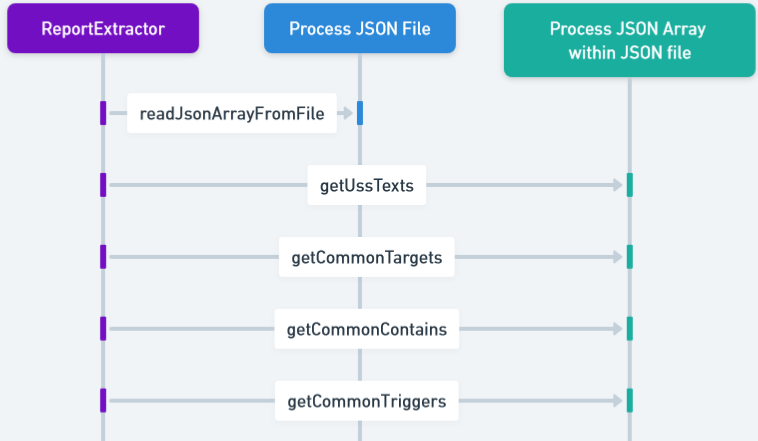
\includegraphics[scale=0.35]{data_extractor_diagram}
%\caption{Sequence diagram for the processes of extracting common entries between two USs from dataset of the %backlog}\label{fig:json_data_extractor_diagram}
%\end{figure} 

The following methods in the ReprortExtractor class are responsible for extracting data from dataset within JSON file:
\begin{itemize}
	\item readJsonArrayFromFile: This method receives a JSON file as input. After reading, the JSON content is tokenised, parsed into a JSON array and the parsed JSON array is returned.
	
	\item getUSsTexts: This method ensures that the text of the specified US-pair is retrieved from the JSON file and properly assigned to the RedundancyItems object for further processing. It receives a US-pair and RedundancyItems as input. 
	
	It reads a JSON array from a file using the \textit{readJsonArrayFromFile} method, iterates over each JSON object in the array and compares the extracted US identifier with the US identifier extracted from the input US-pair. If a match is found, the text of the first and second USs is set in the redundancyItems object.
	
	\item getCommonTargets: Used to determine overlaps in "Targets" references (pairs of actions and entities) between specified US-pairs from a JSON file.
	
	It receives the identifiers of the US-pair as input. After it finds the US objects, it compares each pair of entries (actions and entities) in "Targets" references of the two USs and looks for matches.
	
	The output is the matches, i.e. the list of common pairs of actions and entities, in "Targets" reference.
	
	\item getCommonContains: Used to determine overlaps in "Contains" references (pairs of entities) between specified US-pairs from a JSON file.
	
	It receives the identifiers of the US-pair as input. After it finds the US objects, it compares each pair of entities in "Contains" references of the two USs and looks for matches.
	
	The output is the matches, i.e. the list of common pairs of entities, in "Contains" reference.
	
	\item getCommonTriggers: Used to determine overlaps in "Triggers" references (pairs of personas and actions) between specified US-pairs from a JSON file.
	
	It receives the identifiers of the US-pair as input. After it finds the US objects, it compares each pair of entries (personas and actions) in "Triggers" references of the two USs and looks for matches.
	
	The output is the matches, i.e. the list of common pairs of personas and actions, in "Triggers" reference.
\end{itemize}
\subsubsection*{Methods for Highlighting Words using Hash Symbol(\#)}
In order to distinguish redundancy words between a US-pair, in text of each US, we decide to highlighting redundant words using hash symbol like \enquote{ ... \#\textless word\textgreater\# ... }.
%Figure \ref{fig:highlight_diagram} is a sequence diagram that illustrates the communication between processes related to the highlighting of redundancy words.
%\begin{figure}[h]
%\centering 
%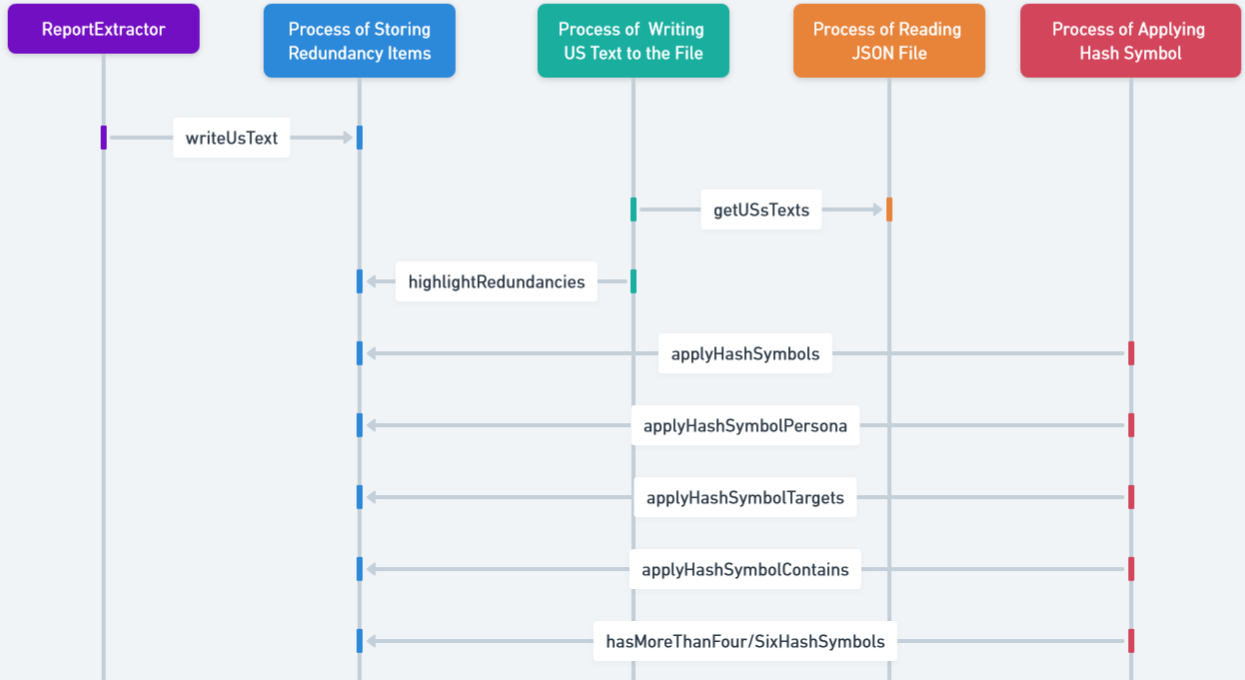
\includegraphics[scale=0.35]{highlight_diagram}
%\caption{Sequence diagram for the process of highlighting redundancy clauses in the Texts of US-pair}\label{fig:highlight_diagram}
%\end{figure} 

The following methods in the ReprortExtractor class are responsible for highlighting redundancy words:
\begin{itemize}
	\item writeUsText: This method reads the text of examined US-pair, highlights redundant element between them using \textit{highlightRedundancies} method, writes the highlighted text to a file, and records information about the redundant elements. 
	
	As input it receive a US-pair, a list of redundant pairs to store redundant pairs in it, an object redundancyItems containing stored redundancy elements and a fileWriter object used for writing output.
	
	It extract the identifier of the two USs from US-pair, retrieves the text of the USs from JSON file and add them to RedundancyItems, invoke the \textit{highlightRedundancies} method to identify and highlight redundants between the USs, it writes the highlighted text of each US to the FileWriter. Finally, sets the redundant pair and count of redundancy clauses.
	\item highlightRedundancies: This method identifies redundancies between US-pair, applies hash symbols using \textit{applyHashSymbols} method to highlight common items and updates the redundancy counts in the redundancyItems object. 
	
	It takes two parameters, redundancyItems and US-pair, which represents the pair of USs to be analysed. 
	
	It checks whether both USs contain a main clause part or whether one of them has a benefit part or whether both USs also have a benefit part.
	
	It applies hash symbols to common elements that only occur in the part of the USs that occurs in the same part (e.g. only main or only benefit part of the USs). 
	
	In each condition, it checks if there are redundancy clauses in the main part, then persona is also highlighted using \textit{applyHashSymbolPersona} method. It also updates the count of main/benefit/total redundancies and sets the changed text of USs. Finally, it returns the updated redundancyItems object.
	\item applyHashSymbols: This method is used to mark certain words within a substring with hash symbols (\#) at the beginning and end to ensure that they are distinguishable and can be easily identified or processed later. 
	
	It takes a substring in which replacements are to be made and a field of matches containing the words to be surrounded with hash symbols. First, the field of matches is sorted in descending order of length and processed accordingly to avoid adding hash symbols to unwanted clauses. 
	\begin{example}
		For example, let's assume that we have \enquote{data} and \enquote{data format} as redundancy elements. If we continue first with \enquote{data} and then with \enquote{import data}, \enquote{import data} will be replaced by \enquote{import \#data\#}, which is not desired.
	\end{example}
	\item hasMoreThanFour/SixHashSymbols: These methods receive a text from the US as input. They are used to check whether there are redundant clauses in the main part of the sentence (it can be one or two clauses). If so, \textit{true} is returned.
	
	\item applyHashSymbolPersona: This method identifies common "Triggers" references, marks them with hash symbols and returns the changed text parts together with the count of redundant triggers references. 
	
	As input, it receives a list of common triggers between US-pair, RedundancyItems and the parts of the USs. It iterates through the list of common triggers and checks whether both elements (persona and primary action) of the triggers are present in both parts. 
	
	It then increments the redundancy count to keep track of the count of redundant triggers. The output returned, is the text of USs containing the manipulated text parts with hash symbols and the redundancy count the in main parts.
	
	\item applyHashSymbolTargets: This method identifies common targets references between two parts of USs, marks them with hash symbols and returns the changed text parts together with the count of redundant targets references.
	
	As input, it receives a list of common targets between the US-pair, RedundancyItems and the parts of the USs. 
	
	It iterates through the list of common targets and checks whether both elements (primary/secondary action and primary/secondary entity) of the targets are present. It then increments the redundancy count in examined part of USs to keep track of the count of redundant targets. 
	
	The output returned is the text of USs containing the manipulated text parts with hash symbols and the redundancy count in examined parts (mains or benefits).
	
	\item applyHashSymbolContains: This method identifies common contains references between two parts of USs, marks them with hash symbols and returns the changed text parts together with the count of redundant contains references. 
	
	As input, it receives a list of common contains between the US-pair, RedundancyItems and the parts of the USs. It iterates through the list of common contains and checks whether both elements of the contains are present in both parts. It then increments the redundancy count to keep track of the count of redundant contains.
	
	The output returned is the text of USs containing the manipulated text parts with hash symbols and the redundancy count in examined parts (mains or benefits).
	
\end{itemize}
\subsubsection*{Methods related to Report Divided Parts of USs}
To show which part of the USs with redundancy words occur between a US-pair, we have split the individual parts of the USs and included them in the report.
%Figure \ref{fig:splitUsText_diagram} is a sequence diagram that illustrates the communication between processes related to the splitting of parts of a US-pair containing redundancy words.
%\begin{figure}[h]
%\centering 
%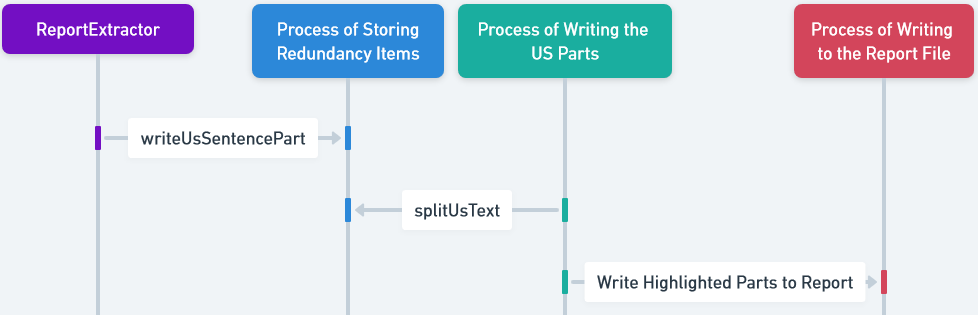
\includegraphics[scale=0.35]{splitUsText_diagram}
%\caption{Sequence diagram for the process of splitting parts of US-pair containing redundancy word}\label{fig:splitUsText_diagram}
%\end{figure} 
The following methods in the ReprortExtractor class are responsible for splitting and reporting the parts of the USs :
\begin{itemize}
	
	\item splitUSsText: This method is used to split the text of two USs into separate sections based on the occurrence of redundancy clauses. 
	
	The input is the text of the first and second US and their corresponding identifiers, a FileWriter for writing to a file and a JSON object for processing JSON data. 
	
	It splits each US text into three parts using commas and saves the result in arrays. It iterates over parts of the first and second USs and searches for occurrences of hash symbol pairs. For each part, the number of hash symbol pairs found is counted. Finally, all parts of the records that contain hash symbols are written to a text file and a JSON file as well.
	
	\item writeUSsSentenceParts: This method facilitates the extraction and storage of highlighted USs parts from US-pair in a textual report file for further analysis.
	
	As input, it receives the US-pair, RedundancyItems and a FileWriter allowing the extracted USs parts to be written. It receives the text of the USs from the redundancyItems object and calls the \textit{splitUsText} method to split the US-pair texts into USs parts with highlighted elements.
	
	The extracted USs parts are also written to the text and JSON report files, using the FileWriter for further processing and analysis.
	
	\begin{example}
		Take, for example, the following US-pair:
		
		\textit{user\_story\_60:} \#g22\# as an it staff member, I want to \#know\# \#how\# the \#data\# is \#used\#, so that I can determine what kind of basic services and functionalities are required.\\\\
		\textit{user\_story\_04:} \#g22\# as a data manager, I want to \#know\# \#how\# the \#data\# is \#used\#, so that I can develop more detailed usage and support scenarios with researchers.\\\\
		The following sentence parts are candidates for possible redundancies between USs:\\\\
		user\_story\_04:  I want to \#know\# \#how\# the \#data\# is \#used\#\\\\
		user\_story\_60:  I want to \#know\# \#how\# the \#data\# is \#used\#	
	\end{example}
\end{itemize}
\subsubsection*{Methods related to Creating Table}
The summary of potential redundancies between US-pairs is presented in a table, which makes it easy to find out which US-pairs have been identified as potentially redundant US-pairs and how many redundancy elements there are in total.
%Figure \ref{fig:writeTable_diagram} is a sequence diagram that illustrates the communication between the processes related to creating tables and addition to text reports.
%\begin{figure}[h]
%\centering 
%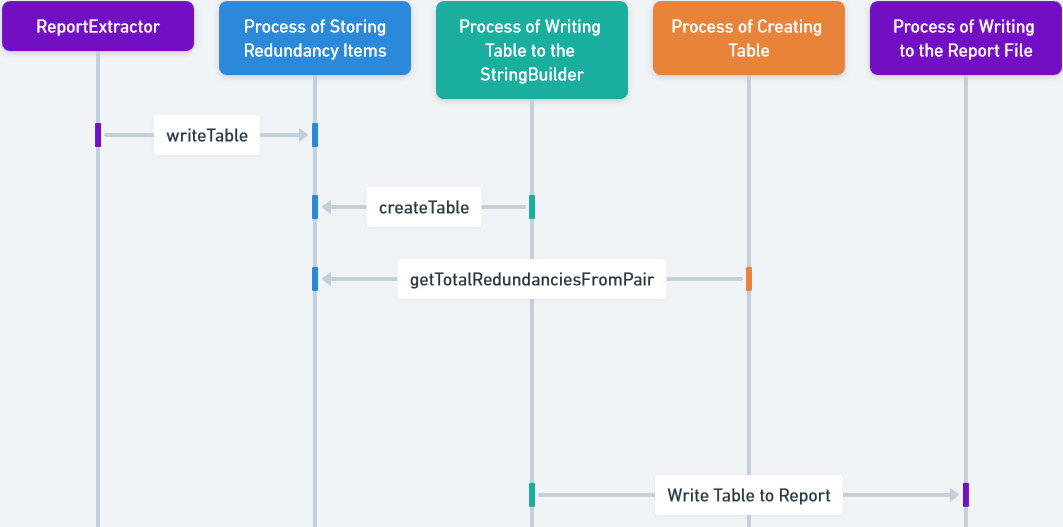
\includegraphics[scale=0.35]{writeTable_diagram}
%\caption{Sequence diagram for the process of creating and adding tables to the textual report}\label{fig:writeTable_diagram}
%\end{figure} 
The following methods in the ReprortExtractor class are responsible for creating a table at the beginning of the text report:
\begin{itemize}
	\item writeTable: This method is used to write a table of potential redundancies between USs and the count of their total redundant clauses using \textit{createTable} method.%, including the addition of the count of main and benefit redundancy clauses using \textit{createTable} method.
	
	As input, it receives a File object into which the table is inserted and a list of redundancy pairs containing information about redundant clauses in US-pairs.
	
	It reads the existing content of the textual report file into a StringBuilder. It creates a table to display the potential redundancies between USs and the count of total redundancy clauses.
	
	The table headers and contents are generated based on the redundant pairs. It calculates the maximum width for each column in the table to ensure proper formatting. Finally, the table content is written to the FileWriter, followed by the existing content stored in the report's StringBuilder.
	
	\item createTable: This method prepares the content for the table in which potential redundancies between USs are displayed, taking into account the total redundancy count between each US-pairs based on the RedundantPair objects provided.
	
	As input, it receives a list of unique US-pairs for which the table is to be created and a list of RedundantPair objects containing information about redundant clauses between US-pairs.
	
	It initialises a two-dimensional array containing the contents of the table. The size of the table is determined by the count of unique pairs of USs plus one for the header row and column.
	
	It fills the header row and the first column of the table with unique pairs of US-pairs, replacing \enquote{user\_story} with \enquote{us} for the purpose of brevity.
	
	It calculates the maximum redundancy count between each US-pair by calling the method \textit{getTotalRedundanciesFromPair}. Finally, it fills the table with the total redundancy count. 
	
	The output is a two-dimensional array representing the contents of the table, with each cell containing the maximum redundancy count between the corresponding pair of USs.
	
	\item getTotalRedundanciesFromPair: This method makes it easier to retrieve the total number of redundancies between a US-pair from a list of RedundantPair objects.
	
	As input, it receives a list of RedundantPair objects containing information about redundant elements in US-pairs, where the first and second USs are to be compared.
	
	It iterates through each RedundantPair object in the RedundantPairs list and checks for each RedundantPair object whether the examined US-pair matches as redundant US-pair. 
	
	If a matching pair is found, the maximum redundancy number stored in this RedundantPair object is returned. If no matching pair is found, \textit{zero} is returned, indicating that there are no redundancies between the examined US-pair.
\end{itemize}
\subsubsection*{Report Evaluation}\label{step_report_evaluation}
The Evaluation class, found in the \textit{org.henshin.backlog.code.evaluation} package, was created to assess redundancy levels in USs based on extracted JSON reports. This class includes methods that evaluate whether two USs are fully or partially redundant, focusing on various application components within these USs.

Figure \ref{fig:evaluation_class_diagram} is a class diagram that illustrates the attributes, operations of the Evaluation class and its relationship to other classes.
\begin{figure}[h]
	\centering 
	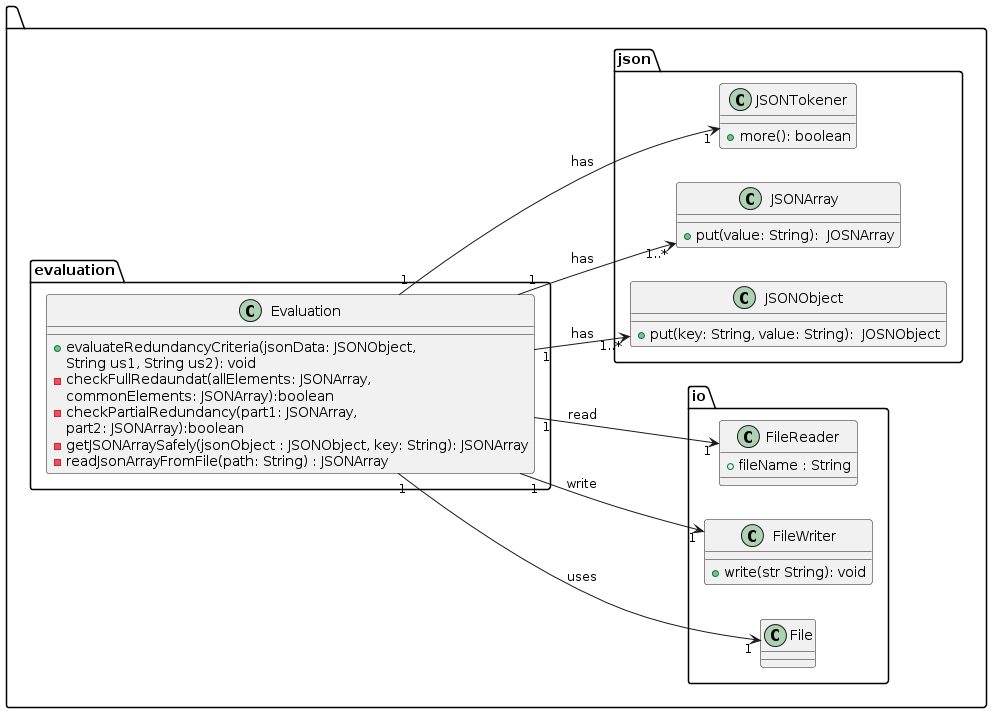
\includegraphics[scale=0.4]{evaluation_class_diagram}
	\caption{Class diagram related to Evaluation class}\label{fig:evaluation_class_diagram}
\end{figure} 
The class offers a detailed mechanism to evaluate redundancies through following methods:
\begin{itemize}
	\item\textit{evaluateRedundancyCriteria}: This method compares elements such as "Triggers", "Targets" and "Contains" in the "Main" and "Benefit" parts of USs. The method checks whether these clauses are fully redundant (i.e. they are identical between USs) or partially redundant (i.e. they share some clauses but are not fully identical).
	
	As input, it receives the JSON object for a specific US-pair.
	
	In particular, it checks various conditions, e.g. whether common clauses are present, whether targets or contains are empty and whether the clauses in the stories are fully or partially identical.
	
	As output, the method updates the JSON report with new keys indicating the redundancy status:
	
	Main Part Fully Redundant: A Boolean value indicating whether the "main part" of the USs is fully redundant.
	
	Main Part Partially Redundant: A Boolean value that indicates whether the "main part" of the USs is partially redundant.
	
	Benefit Part Fully Redundant: A Boolean value that indicates whether the "benefit part" of the USs is fully redundant.
	
	Benefit Partially Redundant: A Boolean value that indicates whether the "benefit part" of the USs is partially redundant.
	
	\item checkPartialRedundancy: The method processes these arrays to identify partial redundancies by checking whether elements from arrays of elements match elements from another array. 
	
	It receives the two arrays of elements as input, iterates through each element of the first input array and compares each of these elements with all elements in the second input array. A match counter records how often elements from the first input array find a match in the second input array.
	
	As output, method returns a boolean value. True: indicates that there is at least one matching element pair between the two JSON arrays, which means partial redundancy. False: indicates that there are no matching elements, indicating no partial redundancy between these specific parts of the USs.
	
	\begin{example} Let's assume we have the following JSON arrays for two different USs: \\\\
		First JSON array: [["login", "button"], ["help", "link"]]\\
		Second JSON array:	[["logout", "button"], ["help", "link"]]\\\\
		The method would determine that the second element of the first array ("help", "link") matches the second element of the second array. As there is at least one match, checkPartialRedundancy would return true, indicating partial redundancy.
	\end{example}
	
	
	\item getJSONArraySafely: This method is designed to handle JSON operations safely by retrieving JSON array from a JSON object without the risk of throwing exceptions if the specified key does not exist.
	
	As input it receives the JSON object from which the JSON array needs to be extracted and a key corresponding to the JSON array within the provided JSON object.
	
	The method first checks whether the provided key exists in the JSON object. If the key exists, it retrieves the JSON array associated with that key. If the key does not exist, it returns an empty JSON array.
	\begin{example} Let's assume that a JSON object representing US's details should contain the key for "Benefit Part", which does not exist:\\
		\{\\
		"Common Targets" : \{\\
		"Main Part" : [["login","button"],["help","link"]]
		\}\\
		\} \\\\
		If the "Benefit Part" in the "Common Targets" needs to be accessed that does not exist, this is handled safely with \textit{getJSONArraySafely} by returning an empty array to avoid runtime errors.
	\end{example}
	
	\item readJsonArrayFromFile: The method enables JSON data to be read from a file and converted into a JSON array object. It takes the file path as input and attempts to open the file, checking whether the file is empty or missing. If the file is available and contains data, this data is read, converted into a JSON array object and returned.
	
\end{itemize}
\subsubsection*{Error Handling}
There were erroneous data in datasets that force us to handle them correctly. Therefore, we implement/use the following exceptions to accurately distinguish and handle them.

The following classes, which extend the \textit{Exception} class, are used in the \textit{org.henshin .backlog.code.rule} package and concern error handling related to the JSON entries in the dataset of the backlogs and the Ecore meta model required to create the rules based on them:
\begin{itemize}
	\item EmptyOrNotExistJsonFile: Is triggered if the JSON file could not be found in the file system.
	
	\item ActionInJsonFileNotFound: Is triggered if the entry \textit{Action}, which contains \textit{Primary/Secondary Actions}, is not present in the JSON file and its absence should be reported.
	
	\item EntityInJsonFileNotFound: Is triggered if the entry \textit{Entity}, which contains \textit{Primary/Secondary Entity}, is not present in the JSON file and its absence should be reported.
	
	\item PersonaInJsonFileNotFound: Is triggered if the entry \textit{Persona} does not exist in the JSON file for a specific US.
	
	\item TextInJsonFileNotFound: Is triggered if the entry \textit{Text} does not exist in the JSON file for a specific US. 
	
	\item UsNrInJsonFileNotFound: Is triggered if the entry \textit{Us\_Nr} does not exist in the JSON file for a specific US.

	\item EdgeWithSameSourceAndTarget: Refers to the creation of edges in graph transformation rules and is triggered if the source and target of the edge have already been created, then the duplicate edge should be avoided.
		
	\item TargetsInJsonFileNotFound: Is triggered if the entry \textit{Targets} does not exist in the JSON file for a specific US.
	
	\item ContainsInJsonFileNotFound: Is triggered if the entry in \textit{Contains} is not present as \textit{Primary/Secondary Entity} in the JSON file and its absence should be reported.
	
	\item TriggersInJsonFileNotFound: Is triggered if the entry \textit{Triggers} does not exist in the JSON file for a specific US. 
	
	\item EcoreFileNotFound: Is triggered if the required Ecore meta-model file could not be found and should also be reported.
\end{itemize}
Within the \textit{org.henshin.backlog.code.report} package, special classes that extend the \textit{Exception} class are designed to solve problems related to the CDA report directory, which encapsulates all US-pairs together with the associated conflict reasons. These classes include:
\begin{itemize}
	\item CdaReportDirIsEmpty: This exception is called if the CDA report directory is found but has no content.
	\item CdaReportDirIsNotADirectory: This exception is thrown in scenarios where the path provided for the CDA report directory is either not a directory (i.e. it is a file) or the specified path does not lead to a directory.
	\item CdaReportDirNotFound: This exception is triggered if the CDA report directory cannot be found within the specified path.
\end{itemize}
\subsubsection*{Limitations}
There are technical limitations that are forcing us to change our implementation strategy.
The following limitations should be clarified at the beginning:
\begin{itemize}
	\item Use Eclipse version 2023-03, as Henshin version 4 cannot be installed with the latest version of Eclipse.
	
	\item Working with Java as the programming language, as the Henshin and CDA APIs are only available in the Java programming language.
	
	\item CDA API is not yet implemented to take into account conflicts and dependencies for \textit{attributes} that are crucial for our approach. This forces us to use the CDA graphical user interface(GUI) instead of the CDA API.
	
	\item Lack of Henshin documentation regarding methods and classes, which makes it time consuming to understand the methods and make the right decision.
\end{itemize}
\subsection{Test}\label{redundancy_test}
In this section, we aim to validate certain functionalities, check the system requirements and ensure reliability and robustness of implemented classes and methods. 

As a test strategy, we perform unit tests with \textit{JUnit} version 4\footnote{\href{https://junit.org/junit4/}{https://junit.org/junit4/}} as version 4 is more suitable and compatible with Eclipse version 2023-03.

EclEmma\footnote{\href{https://www.eclemma.org/}{https://www.eclemma.org/}} as a code coverage tool integrated into the Eclipse IDE is used, to ensure thorough testing and coverage. By using EclEmma, we were able to systematically measure the effectiveness of our test suites and determine the test coverage for each individual class.
\subsubsection*{Configuration of Test Environment}
In the main project \textit{org.henshin.backlog}, we create a separate package called \textit{org.henshin. backlog.test}. This package contains three Java classes namely \textit{ReportExtractorTest.java}, \textit{RuleCreator\_Test.java}, and \textit{EvaluationTest.java}, each of which corresponds to the Java source codes accordingly.
\subsubsection*{Scope of Testing}
The scope of the test depends on the system requirements and the three most important implemented classes \textit{ReportExtractorTest.java}, \textit{RuleCreator\_Test.java}, \textit{Evaluation.java} and their methods. The implemented error handling classes are also tested.
\subsubsection*{Test Cases and their Code Coverage}
We describe the specific test cases that are performed during the tests. Each test case contains a description of the test scenario, the data provided and the expected result. For refining and improving our test cases, we used a code coverage report created by EclEmma in order to increase coverage and ensure a more reliable, error-resistant application.

Table \ref{tb:test_cases_rule_creator} shows the test cases for the RuleCreator.java class and Figure \ref{fig:code_coverage_rule_creator} shows the code coverage.

%\newgeometry{margin=2.5cm}
%\begin{landscape}
\thispagestyle{empty}
%\begin{figure}[h]
\begingroup
\centering
\scriptsize
\renewcommand{\arraystretch}{1,5} 
\keepXColumns
	\begin{tabularx}{\textwidth}{X  X  X  X}
	\hline
	Test Case &Supplied Data&Expected Outcome&Description\\
	\hline\hline
	\endfirsthead
	\hline
	Test Case &Supplied Data&Expected Outcome&Description\\
	\hline\hline
	\endhead
		testAssignCmodule&Assign a dummy ECore model file&Through an exception: \textit{EcoreFileNotFound}&Check whether the ECore model already exists and CModule is correctly assigned\\
		
		ActionNotExist\newline (testProcessJsonFile)&JSON file with a US without \enquote{Action} entry&Through an exception:  \textit{ActionInJsonFileNotFound}&Check whether there is an entry \enquote{Action} in the related US in JSON file\\
		
		
		EntityNotExist\newline (testProcessJsonFile)&JSON file with a US without \enquote{Entity} entry&Through an exception: \textit{EntityInJsonFileNotFound}&Check whether there is an entry \enquote{Entity} in the related US in JSON file\\
		
		PersonaNotExist\newline (testProcessJsonFile)&JSON file with a US without \enquote{Persona} entry&Through an exception: \textit{PersonaInJsonFileNotFound}&Check whether there is an entry \enquote{Persona} in the related US in JSON file\\
		
		TargetsNotExist\newline (testProcessJsonFile)&JSON file with a US without \enquote{Targets} entry&Through an exception: \textit{TargetsInJsonFileNotFound}&Check whether there is an entry \enquote{Targets} in the related US in JSON file\\
		
		ContainsNotExist\newline (testProcessJsonFile)&JSON file with a US without \enquote{Contains} entry&Through an exception: \textit{ContainsInJsonFileNotFound}&Check whether there is an entry \enquote{Contains} in the related US in JSON file\\
		
		ContainsInTargets\newline (testProcessContainsEdges)&JSON file with a US which the entity in \enquote{Targets} entry also serves as containment&The entity in Contains should be annotated as \textless delete\textgreater&Check whether entity in Targets have connection as Contains, if so entity in Contains should also annotated as \textless delete\textgreater\\
		
		TriggersNotExist\newline (testProcessJsonFile)&JSON file with a US without \enquote{Triggers} entry &Through an exception: \textit{TriggersInJsonFileNotFound}&Check whether there is an entry \enquote{Triggers} in the related US in JSON file\\
		
		DuplicateTriggers\newline (testProcessContainsEdges)&JSON file with a US with duplicate Triggers entries&Through an exception: \textit{EdgeWithSameSource AndTarget}&Verify whether there is duplicated entries in Triggers JSON-array\\
		
		TextNotExist\newline (testProcessJsonFile) &JSON file with a US without \enquote{Text} entry&Through an exception: \textit{TextInJsonFileNotFound}&Check whether there is an entry \enquote{Text} in the related US in JSON file\\
		
		UsNrNotExist\newline (testProcessJsonFile)&JSON file with a US without \enquote{Us\_Nr} entry&Through an exception: \textit{UsNrInJsonFileNotFound}&Check whether there is an entry \enquote{US\_Nr} in the related US in JSON file\\
		
		UndefindedEntity\newline (testProcessContainsEdges)&Specify an entity that is not contained as \enquote{Entity} in the JSON file, but appears as \enquote{Contains}&Through an exception:  \textit{EntityInJsonFileNotFound}&Check whether the entity that appears in the \textit{Contains} entry has already been identified as an entity\\
		
		PrimaryActionNotFound \newline(testProcessTargetsEdges)&Specify a primary action that is not contained as \enquote{Primary Action} in the JSON file, but appears as \enquote{Targets}&Through an exception: \textit{ActionInJsonFileNotFound}&Check whether the primary action that appears in the \textit{Targets} entry has already been identified as a primary action\\
		
		PrimaryEntityNotFound \newline(testProcessTargetsEdges)&Specify a primary entity that is not contained as \enquote{Primary Entity} in the JSON file, but appears as \enquote{Targets}&Through an exception: \textit{EntityInJsonFileNotFound}&Check whether the primary entity that appears in the \textit{Targets} entry has already been identified as a primary entity\\
		
		SecondaryActionNotFound \newline(testProcessTargetsEdges)&Specify a secondary action that is not contained as \enquote{Secondary Action} in the JSON file, but appears as \enquote{Targets}&Through an exception: \textit{ActionInJsonFileNotFound.class}&Check whether the secondary action that appears in the \textit{Targets} entry has already been identified as a secondary action\\
		
		SecondaryEntityNotFound \newline(testProcessTargetsEdges)&Specify a secondary entity that is not contained as \enquote{Secondary Entity} in the JSON file, but appears as \enquote{Targets}&Through an exception: \textit{EntityInJsonFileNotFound.class}&Check whether the secondary entity that appears in the \textit{Targets} entry has already been identified as a secondary entity\\
		
		UndefindedEntity\newline (testProcessTargetsEdges) &Specify an entity that is not contained as \enquote{Entity} in the JSON file, but appears as \enquote{Targets}&Through an exception:  \textit{EntityInJsonFileNotFound}&Check whether the entity that appears in the \textit{Targets} entry has already been identified as an entity\\
		
		ActionNotFound&Provision of a JSON file that contains actions in \textit{Targets} that are not entered in primary/secondary action&Through an exception:  \textit{EntityInJsonFileNotFound}&Verify whether the action that appear in the \textit{Targets} entry has already been identified as an action\\
		
		ReadJsonArrayFromFile&Assign a dummy JSON file&Through an exception:  \textit{EmptyOrNotExistJsonFile}&Check whether the JSON file already exists\\
		
		EmptyOrNotExistJsonFile&Assign an empty JSON file&Through an exception: \textit{EmptyOrNotExistJsonFile}&Check whether the JSON file is empty\\
		\hline
		\caption{Test cases for RuleCreator  class}\label{tb:test_cases_rule_creator}
	\end{tabularx}
	%\captionof{table}{Test cases for RuleCreator  class}\label{tb:test_cases_rule_creator}
\endgroup

\begin{figure}[h]
	\centering
	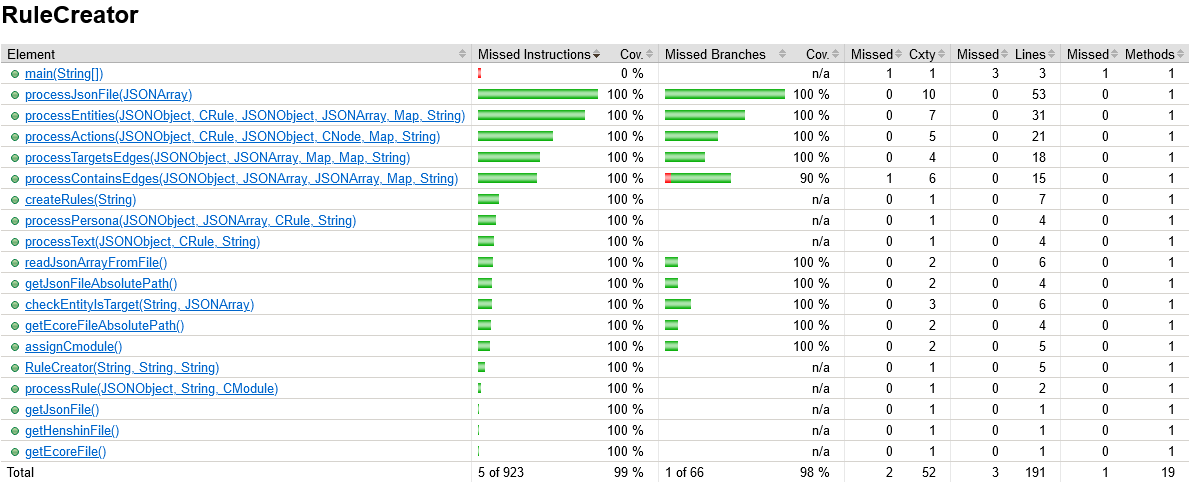
\includegraphics[scale=0.35]{code_coverage_rule_creator}
	%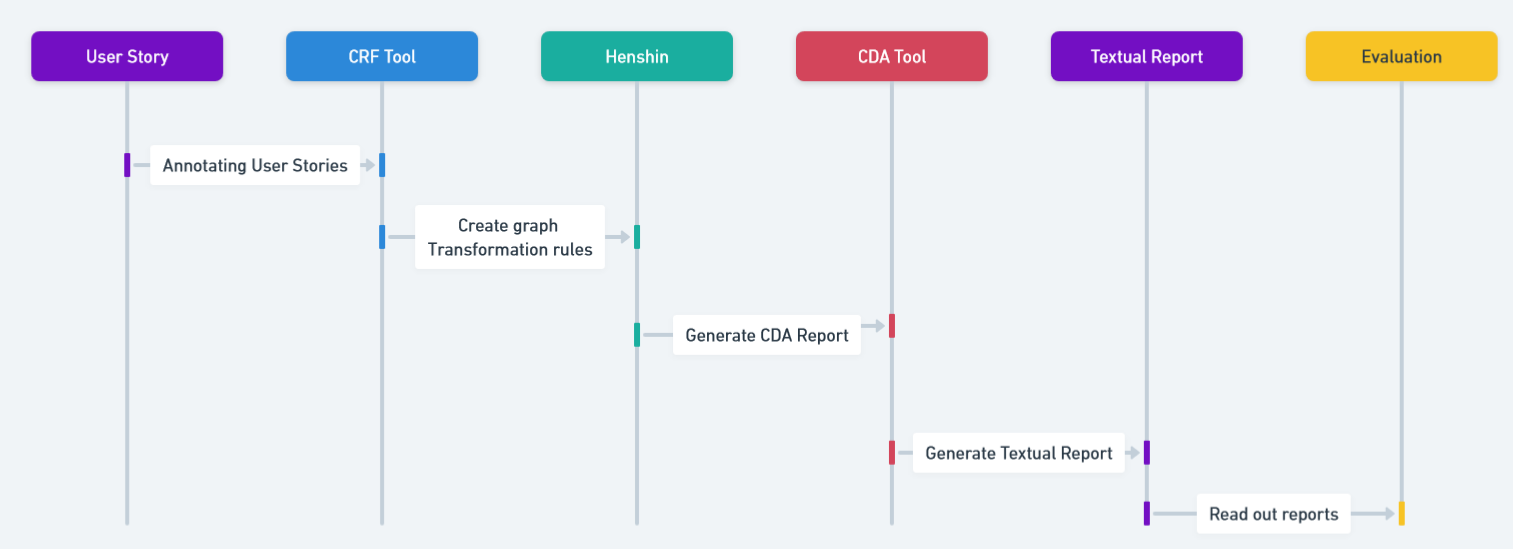
\includegraphics[scale=0.35]{sequence_diagram}
	\caption{Code coverage related to class RuleCreator}\label{fig:code_coverage_rule_creator}
\end{figure} 
Table \ref{tb:test_cases_report_extractor} shows the test cases for the ReportExtractor.java class and Figure \ref{fig:code_coverage_report_extractor} shows the code coverage.

%\end{figure}
%\end{landscape}
%\restoregeometry
%\newgeometry{margin=2.5cm}
%\begin{landscape}
	\thispagestyle{empty}
%	\begin{figure}[h]
		\begingroup
		\centering
		\scriptsize
		\renewcommand{\arraystretch}{1,5} 
		\keepXColumns
		\begin{tabularx}{\textwidth}{X  X  X  X}		
			\hline
			Test Case &Supplied Data&Expected Outcome&Description\\
			\hline\hline
			\endfirsthead
			\hline
			Test Case &Supplied Data&Expected Outcome&Description\\
			\hline\hline
			\endhead
			testEmptyDirectroy&Assign a dummy directory&Through an exception: \textit{CdaReportDirIsEmpty}&Check if CDA Report directory is empty\\
			
			testEmptyJSONFile&Assign an empty JSON dataset file&Through an exception: \textit{EmptyOrNotExistJsonFile}&Check if JSON dataset file is empty\\
			
			testCdaDirNotADirectroy&Assign a file instead of CDA directory&Through an exception: \textit{CdaReportDirIsNotA Directory}&Check if assigned path is a directory\\
			
			testCdaDirectroy&Assign a not readable directory&Through an exception: \textit{CdaReportDir NotFound}&Check whether CDA directory is accessible\\
			
			testFinalReportDir&Assign an empty dataset directory&Return \textit{false} if the assigned directory is empty&Check if directory of datasets are empty\\
			
			testMinimalEcoreExist&Assign a CDA directory without minimal-ecore file&Return \textit{false} if the minimal-ecore file not found&Check whether the Ecore file already exist in CDA directory\\
			
			testWriteTable&Provide a CDA report for a US-pair&A table should be created in the report file&Check whether the table for US-pairs has already been created\\
			
			completeMajorElements \newline Edge\newline(testExtractReports)&Provision of a CDA report for US-pair with exactly one redundant \enquote{Targets} clause&Inclusion of this US-pair in the redundancy report with the entries \enquote{Action}, \enquote{Entity} and \enquote{Targets} &Verifies \textit{extractReports} method when all major elements are present in the CDA report\\
			
			completeMajorElements\newline Upper Edge\newline(testExtractReports)&Provide a CDA report for a US-pair with at least one \enquote{Targets} clause and redundant elements such as Triggers&Generated redundancy report contains information about Secondary Entities, Secondary Actions, Targets, and Triggers&Verifies \textit{extractReports} method when all major elements are present in the CDA report and the up	per edge case is reached\\
			
			notCompleteMajor\newline Elements\newline(testExtractReports)&Provide a CDA report for a US-pair without \enquote{Targets} edge, but with action and entity&The US-pair should not be reported&Verifies the behaviour of the \textit{extractReports} method when not all major elements are present in the input data\\
			
			getBenefitPart\newline RedundanciesElements\newline(testExtractReports)&Provision of a CDA report for a US-pair that only contains redundancy clauses in the \enquote{Benefit} part&Check whether the count of redundancy clauses in the benefit part of the USs matches the value \enquote{Benefit Part Redundancy Clause} specified in the
			JSON\_Report file&Verifies the behaviour of the \textit{extractReports} method when there are redundancy elements in the benefit part of USs\\
			
			getMainPartRedundancies\newline Elements\newline(testExtractReports)&Provision of a CDA report for a US-pair that only contains redundancy clauses in the \enquote{Main} part&Check whether the count of redundancy clauses in the main part of the USs matches the value \enquote{Main Part Redundancy Clause} specified in the JSON\_Report file&Verifies the behaviour of the \textit{extractReports} method when there are redundancy elements only in the main part of USs\\
			
			getTotalRedundancy\newline Elements\newline(testExtractReports)&Provision of a CDA report for a US-pair that contains redundancy clauses in the \enquote{Main}and \enquote{Benefit} parts&Check whether the count of redundancy clauses in the main and benefit parts of the USs matches the value \enquote{Total Redundancy Clause} specified in the JSON\_Report file&Verifies the behaviour of the \textit{extractReports} method when there are redundancy elements in the main and benefit parts of USs\\
			
			highlightPersona\newline(testExtractReports)&Providing a CDA report for a US-pair with redundancy clauses in \enquote{Triggers} (from Persona to Primary Action) and Targets&The persona should also be marked with hash symbol if there is a redundant targets clause in the main part&Checks the behaviour of the \textit{extractReports} method when highlighting redundant persona in USs\\
				
			BenefitInBothUSs\newline(testHlightRedundancies)&Provision of a CDA report for a US-pair where both USs have the \enquote{benefit} part&Search both the main and the benefit parts of USs and mark redundancy clauses with a hash symbol if they occur&Verifies the behaviour of the \textit{highlightRedundancies} method when both USs have benefit parts\\
			
			noBenefitInBothUSs\newline(testHlightRedundancies)&Provision of a CDA report for a US-pair where both USs do not have the \enquote{benefit} part&Search only the main part of USs and mark redundancy clauses with a hash symbol&Verifies the behaviour of the \textit{highlightRedundancies} method when both USs don't have benefit parts\\
			
			noBenefitInUS1\newline(testHlightRedundancies)&Provision of a CDA report for a US-pair where only the second US have the \enquote{benefit} part&Search only the main part of USs and mark redundancy clauses with a hash symbol&Verifies the behaviour of the \textit{highlightRedundancies} method when only the second US have benefit part\\
			
			noBenefitInUS2\newline(testHlightRedundancies)&Provision of a CDA report for a US-pair where only the first US have the \enquote{benefit} part&Search only the main part of USs and mark redundancy clauses with a hash symbol&Verifies the behaviour of the \textit{highlightRedundancies} method when only the first US have benefit part\\
			
			ContainInBenefitPart\newline(testHighlightRedundancies)&Provide a CDA report for a US-pair with redundancy clauses of \enquote{Contains} within \enquote{Benefit} part&The entities included in Contains should be marked with hash symbol&Checks the behaviour of the \textit{highlightRedundancies} method when highlighting redundant entities included in the Contains\\
			
			ContainInMainPart\newline(testHighlightRedundancies)&Provide a CDA report for a US-pair with redundancy clauses of \enquote{Contains} within \enquote{Main} part&The entities included in Contains should be marked with hash symbol&Checks the behaviour of the \textit{highlightRedundancies} method when redundant entities detected in the Contains\\
			
			TargetsInMainPart \newline(testHighlightRedundancies)&Provide a CDA report for a US-pair with redundancy clauses with more than one \enquote{Targets} within the \enquote{Main} part&Founded redundancy clauses should also be marked with a hash symbol, if the main part contains more than one redundancy clause as Targets&Check the behaviour of the \textit{highlightRedundancies} method if there are more than one redundancy clause as Targets in main part\\
			
			TargetsInBenefitPart \newline(testHighlightRedundancies)&Provide a CDA report for a US-pair with redundancy clauses with more than one \enquote{Targets} within the \enquote{Benefit} part&Founded redundancy clauses should also be marked with a hash symbol, if the benefit part contains more than one redundancy clause as Targets&Check the behaviour of the \textit{highlightRedundancies} method if there are more than one redundancy clause as Targets in benefit part\\
			
			
			\hline
				\caption{Test cases for ReportExtractor  class}\label{tb:test_cases_report_extractor}
		\end{tabularx}		
	%	\captionof{table}{Test cases for ReportExtractor  class}\label{tb:test_cases_report_extractor}
		\endgroup
	%\end{figure}

\begin{figure}[h]
	\centering
	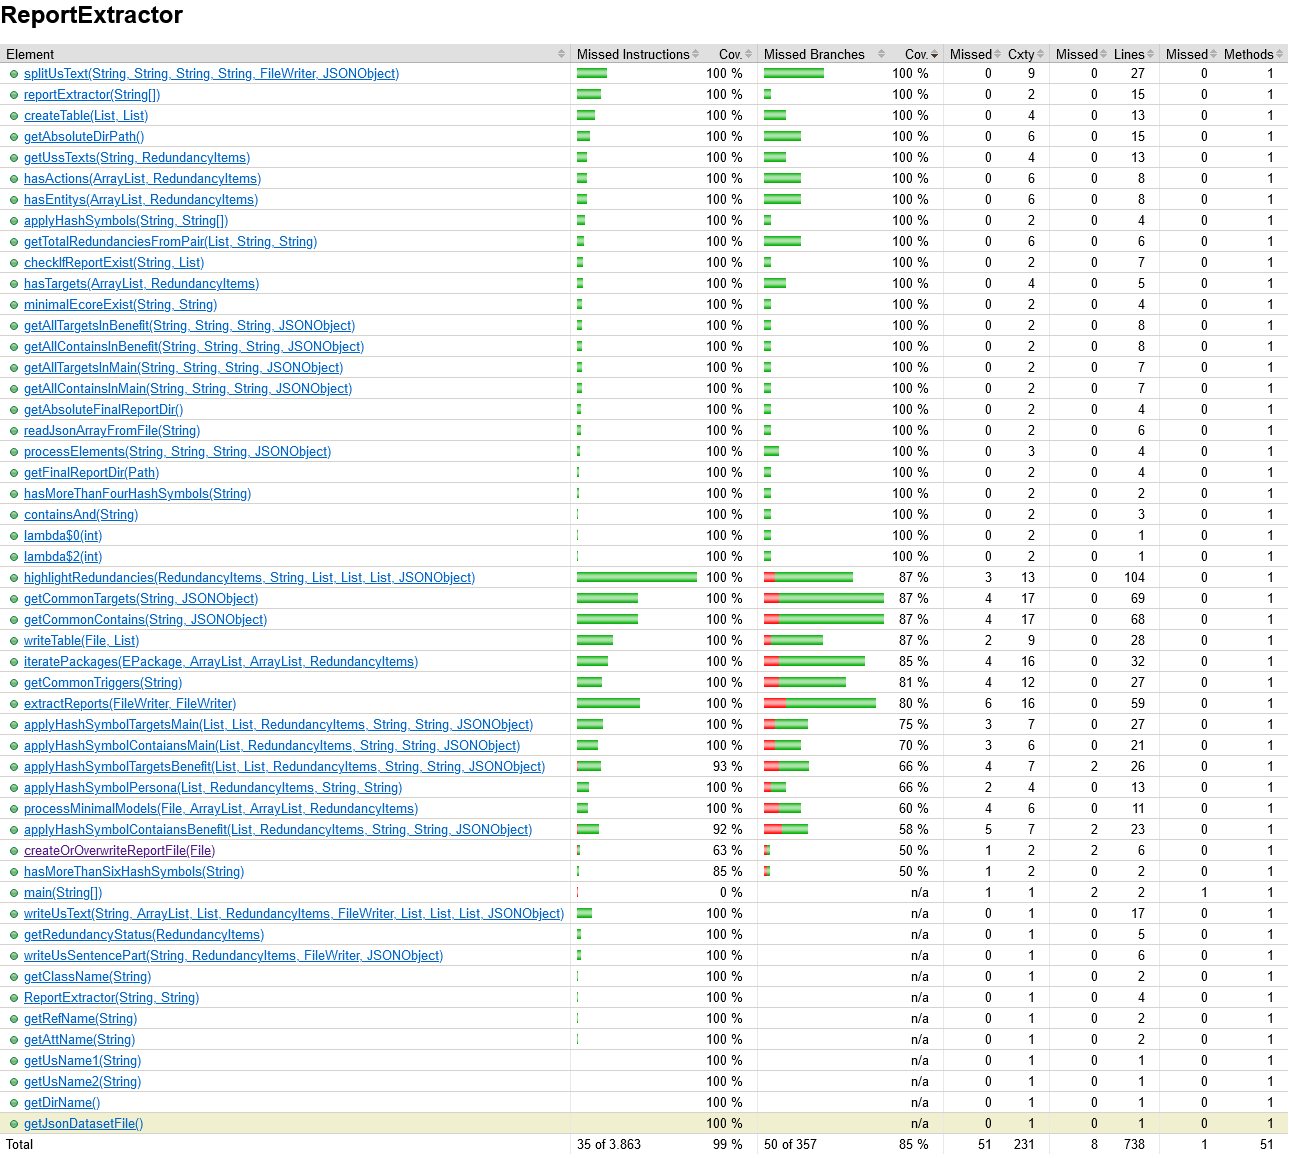
\includegraphics[scale=0.3]{code_coverage_report_extractor}
	\caption{Code coverage related to class ReportExtractor}\label{fig:code_coverage_report_extractor}
\end{figure} 

Table \ref{tb:test_cases_evaluation} shows the test cases for the Evaluation.java class and Figure \ref{fig:code_coverage_evaluation} shows the code coverage.

%\newgeometry{margin=2.5cm}
%\begin{landscape}
%\thispagestyle{empty}
%\begin{figure}[h]
\begingroup
\centering
\scriptsize
\renewcommand{\arraystretch}{1,5} 
\keepXColumns

\begin{tabularx}{\textwidth}{X  X  X  X}
	\hline
	Test Case &Supplied Data&Expected Outcome&Description\\
	\hline\hline
	\endfirsthead
	\hline
	Test Case &Supplied Data&Expected Outcome&Description\\
	\hline\hline
	\endhead
	
	testEmptyOrNotExist JsonFile&Provision of a dummy JSON file&Through an exception: \textit{EmptyOrNotExist JsonFile}&Check whether the provided JSON file already exists and is not empty\\
	
	testJsonFile&Provision of a JSON file which is not accessible&Through an exception: \textit{IOException}&Check whether the provided JSON file is accessible\\
	
	main/benefitFull\_Case1&Provide a JSON file with US-pair that have no common \textit{Contains} entries but have common \textit{Targets} entries in main/benefit parts&In JSON report the entry "Main/Benefit Part Fully Redundant" should be \textit{true}&Check whether US-pair without \textit{Contains} entries can also be fully redundant in main/benefit parts\\
	
	main/benefitFull\_Case2&Provide a JSON file with US-pair that have not common \textit{Contains} entries but one US has entries as Contains in main/benefit&In JSON report the entry "Main/Benefit Part Fully Redundant" should be \textit{true}&Check whether US-pair without common \textit{Contains} entries can also be fully redundant in main/benefit parts\\
	
	main/benefitFull\_Case3&Provide a JSON file with US-pair that have common \textit{Contains} entries but one US have additional entries as Contains in main/benefit parts&In JSON report the entry "Main/Benefit Part Fully Redundant" should be \textit{true}&Check whether USs with additional \textit{Contains} entries from common contains can also be fully redundant in main/benefit parts\\
		
	main/benefitFull\_Case4&Provide a JSON file with US-pair that have exactly common \textit{Contains} entries as well as common \textit{Targets} in main/benefit parts&In JSON report the entry "Main/Benefit Part Fully Redundant" should be \textit{true}&Check whether USs with \textit{Contains} and \textit{Targets} entries can also be fully redundant in main/benefit parts\\
	
	mainBenefitFull&Provide a JSON file with US-pair that all clauses in the main and benefit parts are identical&The JSON report the entries "Main Part Fully Redundant" and "Benefit Part Fully Redundant" should be \textit{true}&Check that all clauses in the main and benefit part are identical, main and benefit part are evaluated as fully redundant\\
	
	mainPartial\_Case1&Provide a JSON file with a US-pair whose entries in \textit{Targets} are partially identical&In the JSON report, the entry "Main Part Partially Redundant" should be \textit{true}&Check whether USs with partially redundant entries in \textit{Targets} are evaluated as partially redundant\\
	
	mainPartial\_Case2&Provide a JSON file with a US-pair whose entries in \textit{Contains} are partially identical&In the JSON report, the entry "Main Part Partially Redundant" should be \textit{true}&Check whether USs with partially redundant entries in \textit{Contains} are evaluated as partially redundant\\
	
	benefitParial&Provide a JSON file with US-pair where only some clauses in \textit{Targets} and \textit{Contains} entries in benefit parts are common&In the JSON report, the entry "Benefit Part Partially Redundant" should be \textit{true}&Check whether USs with partially common \textit{Targets} and \textit{Contains} entries in benefit parts are evaluated as partially redundant\\
	
	mainFullBenefitPartial&Provide a JSON file with US-pair where all clauses in the main parts and some in the benefit parts are identical&In the JSON report, the entry "Main Part Fully Redundant" and "Benefit Part Partially Redundant" should be \textit{true}&Check whether the main parts are evaluated as fully redundant if all clauses are identical and the benefit parts are evaluated as partially redundant if some clauses are identical\\
	
	mainPartialBenefitFull&Provide a JSON file with US-pair where some clauses in the main parts and all in the benefit parts are identical&In the JSON report, the entry "Main Part Partially Redundant" and "Benefit Part Fully Redundant" should be \textit{true}&Check whether the main parts are evaluated as partially redundant if some clauses are identical and the benefit parts are evaluated as fully redundant if all clauses are identical\\
	
	\hline
	\caption{Test cases for Evaluation  class}\label{tb:test_cases_evaluation}
\end{tabularx}

%\captionof{table}{Test cases for RuleCreator  class}\label{tb:test_cases_rule_creator}
\endgroup
\thispagestyle{empty}
%\end{landscape}
%\restoregeometry

\begin{figure}[h]
	\centering
	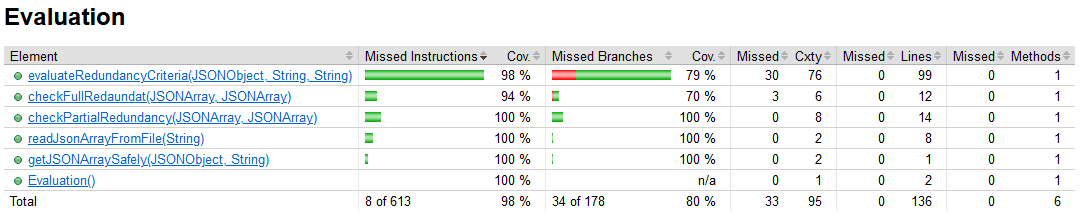
\includegraphics[scale=0.45]{code_coverage_evaluation}
	%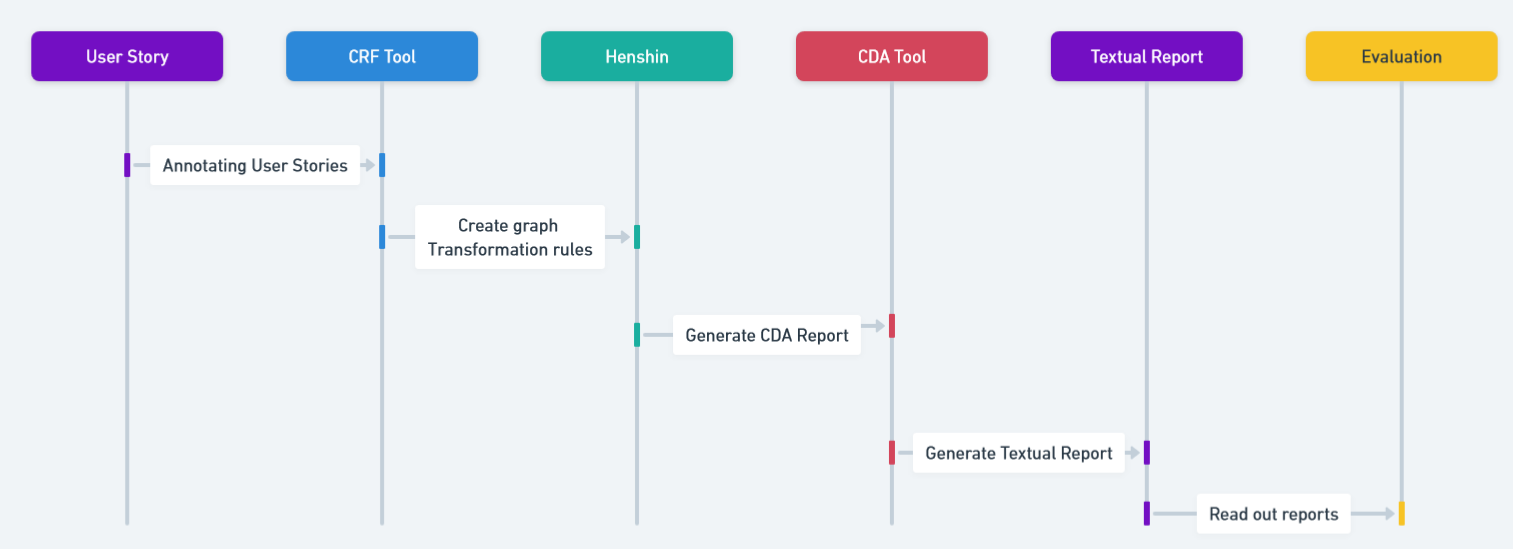
\includegraphics[scale=0.35]{sequence_diagram}
	\caption{Code coverage related to class Evaluation}\label{fig:code_coverage_evaluation}
\end{figure}
%\subsubsection*{Performance Test}
%In this section, we describe the performance testing approach used for this project, including the test setup, key metrics, and the results of the tests.

\subsection{Evaluation}\label{redundancy_evaluation}
%In this section we will present the results of applying our approach to analyse USs in 19 by CRF tool annotated backlog datasets. 
%The purpose of this section is to assess the effectiveness of our approach in analysing redundancy between USs. This section serves several key objective:
In this section, we address two different research questions and provide a detailed explanation of the experimental design and execution for each question. We also present a detailed analysis of the results to provide answers to these research questions, highlight their implications and provide insights into the research findings.
%\begin{itemize}
%	\item Demonstrating the validity and reliability of our proposed methodology for identifying and categorising redundancies between USs.
%	\item Presenting the results of our analysis across multiple datasets, highlighting the prevalence of \enquote{Full and Partial Redundancy} for both the main and benefit parts of USs.
%	\item Gaining insights into the nature and extent of redundancies between USs and its potential impact on software development processes.
%	\item Comparing results from different data sets, identifying patterns or trends and analysing variations in redundancy levels.
%\end{itemize}
\subsubsection*{Research Questions}
The research questions addressed in this section are as follows:
\begin{enumerate}
	\item Does our tool reliably determine the level of redundancy —either partial or full— between different parts of USs (main and benefit)?
	\item How does the tool's performance scale when the number of USs in a backlog increases?
	\end{enumerate}
\subsubsection*{Methodology}
To address the first questions "Does our tool reliably determine the level of redundancy—either partial or full—between different parts of USs (main and benefit)?", we recap the methodology employed to analyse redundancy between USs. We utilized a systematic approach that involved several key steps:
\begin{itemize}
	
	\item Data Collection: For a comprehensive assessment, we applied our approach to 19 backlog datasets presented by Mosser et al.\footnote{https://github.com/ace-design/nlp-stories}. They applied the Doccano approach to these publicly available requirements datasets\cite{requirementsdatasets}.
	
	It is also worth noting that some backlog datasets (g02, g13, g17, g27) did not follow the expected sentence structure, which is why we did not include them in the evaluation results to avoid unexpected behaviour. Table \ref{tb:backlogs} shows the project number of each dataset and the count of USs.
	%	- You have to describe all that in your work, how do you define Main Partial/Full and Benefit Partial/Full, so how do you decide that. And generating this JSON_Report and filling this table is all interesting implementation information.
	
	%When evaluating, I use tools on a large scale and I go through all the cases and look at what comes out of the use case as a meaningful result. As an evaluation, I will enter all the datasets we have as input and then what comes out will be 
	\begingroup
	\centering
	\scriptsize
	\renewcommand{\arraystretch}{1.5} 
	%\keepXColumns
	\begin{tabularx}{\linewidth}{l|XXXXXXXXXXXXXXXXXXX|X}
		Item&	1&	2&	3&	4&	5&	6&	7&	8&	9&	10&	11&	12&	13&	14&	15&	16&	17&	18&	19&	\\
		\hline
		%Project Name&loudoun&recycling&openspending&frictionless&scrumalliance	&nsf&camperplus&datahub&mis&neurohub&alfred&badcamp&rdadmp&archivesspace	&unibath&duraspace&racdam&culrepo&zooniverse&\\
		Project Nr.&	g03	&g04	&g05	&g08	&g10	&g11	&g12	&g14	&g16	&g18	&g19	&g21	&g22	&g23	&g24	&g25	&g26	&g27	&g28	&Total USs\\
		\hline
		Total USs&	57&	51	&53	&66	&97	&73	&54	&67	&66	&102	&137	&69	&83	&56	&53	&100	&100	&114	&60	&1458 \\
		\caption{Project number and count of USs contained in each backlog dataset}\label{tb:backlogs}
	\end{tabularx}	
	\endgroup
	
	%\item Preprocessing: Using the generated JSON report file for each dataset, we create a VBA script called \textit{extractFromJSONFiles}\footnote{https://github.com/amirrabieyannejad/USs\_Annotation/tree/main/Skript/extractFromJSONFiles} to iterate through all the JSON report files and extract the information such as \enquote{US-pair}, \enquote{US-text}, \enquote{total redundancy clauses}, \enquote{main redundancy clauses}, \enquote{benefit redundancy clauses} and \enquote{project number} and collect them all in an Excel file to perform further analyses.
	
	\item Identification of main and benefit parts: Each US was divided into its main part, which is the core functionality, and its benefit part, which describes the value to the persona.
	
	\item Detection of overlapping clauses: Recognition of overlapping clauses between a US-pair in a specific part of the USs.
	
	\item Redundancy analysis in main and benefit parts: Based on the redundant clauses identified, an automatic redundancy analysis was performed for the main and benefit parts of the US-pair based on certain criteria indicating the level of redundancy (partial or full) in the main and benefit parts.
		
	%\item Preprocessing: \item preprocessing: We transform each data set into graph transformation rules, apply CDA and generate a textual report in which each redundancy clause between US-pairs is marked with a hash symbol. Additionally,  the number of founded redundancies in the main and benefit sections is also determined.
\end{itemize}
\subsubsection*{Ground Truth Evaluation of US Redundancy}
Answering the first research question requires our automated system to have a reference point against which its accuracy can be measured. This reference point or "ground truth" is derived from a personal assessment and serves as a benchmark for the tool's performance.

In contrast to the tool evaluation, we did not evaluate based on labels (e.g., action, entity, persona, targets, etc.) in the personal evaluation. This means that when evaluating ground truth, we evaluate partial and full redundancy based on the phrases occurring in a given part as a one-to-one comparison.

The ground truth is the final assessment against which automated results are compared. It is derived from the personal judgement of a subject matter expert (in this case myself) using a combination of expertise, experience and specific evaluation criteria. The personal assessment is targeted at providing a reliable and accurate reference for redundancy between USs.\\\\
	The following criteria were taken into account in the personal assessment:
	\begin{itemize}
		\item A US-pair is evaluated as fully redundant in the main part, if all phrases occurred in the main parts of both USs fully overlap with one-to-one comparison. For example, the following US-pair is assessed as fully redundant:\\
		user\_story\_01: "\#g14\# as a \#publisher\#, i want to \#publish\# a \#dataset\#, so that i can view just the dataset with a few people."
		
		user\_story\_02: "\#g14\# as a \#publisher\#, i want to \#publish\# a \#dataset\#, so that i can share the dataset publicly with everyone."
		
		\item A US-pair is considered fully redundant in the main part, if all phrases in the main part of at least one US completely overlap. For instance:\\
		user\_story\_22: "\#g14\# as a \#consumer\#, i want to \#view\# a \#data package\# online, so that i can \#get\# a \#sense\# of whether this is the dataset i want."
		
		user\_story\_24: "\#g14\# as a \#consumer\#, i want to \#view\# the \#data package\#, so that that i can \#get\# a \#sense\# of whether i want this dataset or not."
		
		\item A US-pair is categorised as partially redundant in the main part if some phrases remain distinctive between the USs. For Instance:\\
		user\_story\_09: "\#g04\# as a \#user\#, i want to be able to \#view\# a \#map display\# of the public recycling bins around my \#area\#."
		
		user\_story\_10: "\#g04\# as a \#user\#, i want to be able to \#view\# a \#map display\# of the special waste drop off sites around my \#area\#."
		
		\item The criteria mentioned were also applied to the benefit part.
	\end{itemize}
Table \ref{tb:ground_truth} shows the aggregation of full and partial redundancies in the main and benefit parts as ground truth.
\begin{figure}[h]
	\begingroup
	\scriptsize
	\centering
	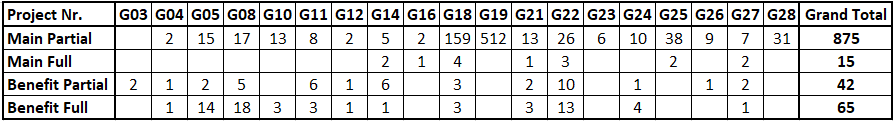
\includegraphics[scale=0.6]{Table/ground_truth.png}
	\captionof{table}{Detail about full and partial redundancies related to main or benefit parts as ground truth}\label{tb:ground_truth}
	
	\endgroup
\end{figure}
As we can see, the main parts of the US-pairs have less full redundancy (15 cases), which means that there are 15 cases where the main part of the US-pairs is exactly the same. This level of redundancy indicates common functionality of the US-pairs, which is a sign of overlapping features. 

A much higher occurrence of partial redundancy in the main parts(875 cases) indicates that there are common elements between the US-pairs, but still enough differences to avoid a complete match. 

Fewer instances of partial redundancy in the benefit parts (42 cases) indicate that the USs diverge in their benefit clauses, they are more tailored to specific project outcomes. 

The higher count of full redundancies (42 cases) compared to partial redundancies in the benefit parts is interesting, as it indicates that the expected objectives of certain features are often repeated in the USs. This suggests that the project is aiming for a set of common goals regardless of the specific functionality.
\subsubsection*{Evaluation of US Redundancy using Tool}
The automated tool is designed to identify redundancy among USs based on predefined criteria. It operates by analysing the text and structure of USs to detect similarities that could indicate redundancy.

In contrast to ground truth, which is based on one-to-one comparison of phrases in specific parts of USs, tool evaluation relies heavily on specified labelling (targets, triggers, contains) using the Doccano tool.

The following criteria are defined for the evaluation of US-pairs:
\begin{itemize}
	\item Full redundancy: 	A pair of US is considered to have "full redundancy" in the main or benefit part when every labelled clause in that part—comprising triggers (in the main part), targets, and contains—is syntactically identical.
	
	\item Partial redundancy: When only some labelled clauses, such as targets, have significant overlap but are not completely identical. This means that while certain labelled clauses, such as targets, may match between USs, other labelled clauses, such as triggers or contains, may differ, meaning that the USs are not fully redundant. This scenario suggests that while USs have significant similarities, they still contain unique aspects.
\end{itemize}
Table \ref{tb:tool} shows the aggregation of the full and partial redundancies in the main and benefit parts assessed by the tool. It is also worth noting that the numbers highlighted in red show the variation in the ground truth evaluation.
\begin{figure}[h]
	\begingroup
	\scriptsize
	\centering
	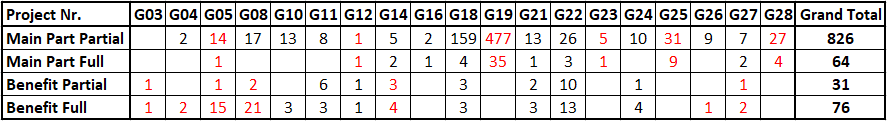
\includegraphics[scale=0.6]{Table/tool.png}
	\captionof{table}{Aggregation of the count of full and partial redundancies in relation to the main or benefit parts assessed by the tool}\label{tb:tool}
	\endgroup
\end{figure}
\paragraph{Assessment of Result: High-Level Overview}Based on the datasets provided, it was found that 1,851 redundancy clauses were identified across all projects, with the highest count found in the backlog G19 dataset (925 clauses), indicating a significant presence of redundancy in the USs of this project. 

Table \ref{tb:redundancy_clauses} shows the total number of redundancy clauses found in each dataset.
\begin{figure}[h]
	\begingroup
	\scriptsize
	\centering
	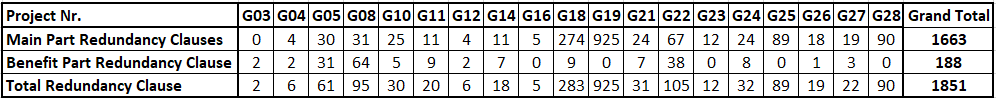
\includegraphics[scale=0.55]{Table/redundancy_clauses.png}
	\captionof{table}{Detail about number of redundancy clauses occurred in main and benefit parts}\label{tb:redundancy_clauses}
	
	\endgroup
\end{figure}
\paragraph{Assessment of Result: Aggregated Analysis}We also look for an aggregate for the count of redundant clauses in both the main and the benefit parts of the USs. 

In the main parts, the large count of full redundancies, especially where two clauses are present (6 clauses), indicates a high degree of similarity in the functionalities described.

In the benefit part of the USs, there is a considerable count of cases where full redundancy prevails, especially where two clauses are inserted (24 clauses). The large count of full redundancies with two clauses indicates that benefits are often described in a standardised way in the different USs.

Figure \ref{fig:aggregation} illustrates the aggregation of the count of redundancy clauses that occur in USs.

\begin{figure}[h]
	\centering
	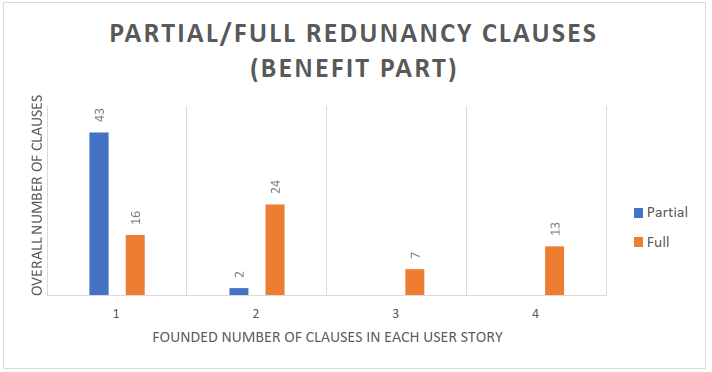
\includegraphics[scale=0.5]{aggregation_benefit}
	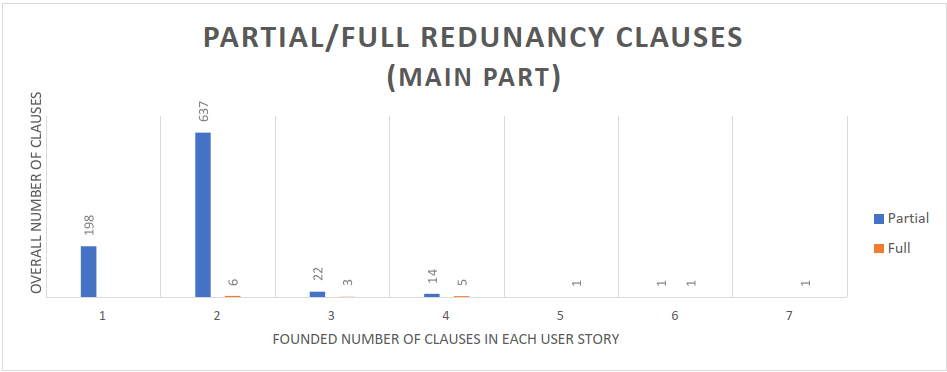
\includegraphics[scale=0.5]{aggregation_main}
	\caption{The aggregation between the count of redundancy clauses occurred in USs}\label{fig:aggregation}
\end{figure}
\paragraph{Assessment of Result: Detailed Insights}In the dataset of Backlog G19, the clause \enquote{have alfred} was repeated in all USs, indicating that \enquote{alfred} is the end product and not a specific functionality. This suggests that the quality of the USs should be considered, so that they do not contain generic information that results in a lot of redundant information(false positives) being provided.

In the main parts of the USs, 1,663 clauses were redundant("Main Part Redundancy Clauses" in Table \ref{tb:redundancy_clauses}), while only 188 redundancy clauses were found in the benefit parts("Benefit Part Redundancy Clauses" in Table \ref{tb:redundancy_clauses}). This means that some USs are not often written in a standardised format for the description of core functions, resulting in a higher count of redundant clauses in the main part.
\begin{example}
	In the dataset of backlog G18 (274 clauses out of 283 in the main parts), for example, this is due to the clauses \enquote{have ability} in the main part, which are unnecessarily repeated in most USs:\\
	\textit{user\_story\_92:} \#g18\# as a \#researcher\# I want to have \#the \#ability\# to search files by file type and format.\\
	\textit{user\_story\_80:} \#g18\# as a \#researcher\# I want to have \#the \#ability\# to attach standard metadata for behavioural observations (and video) so that my data can be searched and understood later.\\
	Actually, the clause \enquote{have ability} in USs should be deleted and no redundancy should be possible at all:\\
	\textit{user\_story\_92:} \#g18\# as a researcher I want to search for files by file type and format.\\
	\textit{user\_story\_80:} \#As a researcher, I want to attach standard metadata for behavioural observations (and videos), so that my data can be searched and understood later.
\end{example}

There are also USs with the same functionality, but one provides more details about the functionality. In other words, one US is contained within another, and we refer to them as full
redundant US-pairs, as deleting the US with less detail has no negative impact on the system. Sometimes it is necessary to merge these two USs to obtain a single detailed US.
\begin{example}
	In the dadaset of backlog G18, for example, we have two US-pairs that are marked as full redundancy between user\_story\_12 and user\_story\_11 as well as user\_story\_13 and user\_story\_11:\\
	\textit{user\_story\_12}: \enquote{\#g18\# as a \#researcher\#, I want to \#upload\# \#files\# prior to having them \#attached\# to a \#log book page\# using the web interface.}\\
	\textit{user\_story\_11:} \enquote{\#g18\# as a \#researcher\#, I want to \#upload\# \#files\# prior to having them \#attached\# to a \#log book page\#.}\\
	\textit{user\_story\_13:} \enquote{\#g18\# as a \#researcher\#, I want to \#upload\# \#files\# prior to having them \#attached\# to a \#log book page\# using a mapped network drive.}\\
	
	As we can see, the user\_story\_11 is an incomplete version of two other USs, and deleting it has no negative impact in the system, due to the fact that its goal is achieved and fulfilled by two other USs.
\end{example}
\paragraph{Research question 1: Conclusion}
After comparing the Ground Truth result with the result provided by our tool, the following realisation was made:
\begin{itemize}
	\item Main Part Partial: A -5.6\% (negative) percentage suggests that the Framework has fewer "Main Part Partial" counts than the Ground Truth.
	In this case, the Framework has about 5.6\% fewer "Main Part Partial" counts than expected.
	
	\item Main Part Full: A high positive percentage of 326.67\% indicates that the Framework has a significantly higher count of Main Part Full compared to Ground Truth.
	At 326.67\%, the framework has more than three times as many main part full compared to the ground truth.
	In our investigation, we found that some phrases are not included as relationship (contains or targets) in the USs annotated with the Doccano tool. Therefore, our tool categorised some USs as fully redundant when in reality they were only partially redundant.
	
	\item Count of Benefit Partial: -26.19\% a negative percentage here indicates that the Framework has fewer "Benefit Partial" counts compared to the Ground Truth.
	With -26.19\%, the Framework has approximately one-quarter fewer "Benefit Partial" counts.
	
	\item Count of Benefit Full: 16.92\% a positive percentage indicates that the Framework has more "Benefit Full" counts compared to the Ground Truth.
	With 16.92\%, the Framework has almost 17\% more "Benefit Full" counts than the Ground Truth.
\end{itemize}
It is also notable that if we add founded partial and full redundancies in main or benefit parts, we both amount are identical(main part: 890 cases , benefit part: 107).

This consistency indicates that the automated tool's results align with the ground truth, suggesting that the tool is reliable in detecting redundancy. It demonstrates that the tool's performance closely matches the personal assessment, reinforcing confidence in its accuracy and validity.
\subsubsection*{Performance Evaluation}
To answer the second research question "How does the tool's performance scale as the count of USs in a backlog increases?", we conducted a series of tests to measure the time it takes the tool to process different counts of USs. This section describes the testing methodology, the results obtained and the impact on the scalability of the tool.
\paragraph{Test Methodology}To evaluate the tool's performance, we conducted a set of experiments in which the tool processed different numbers of USs in a backlog. The tests involved the following steps:
\begin{enumerate}
	\item Backlog Setup: We used backlogs with varying numbers of USs around—50, 70, 90, 120 and 140—to simulate different workload sizes. Each backlog contained USs with varying content, redundancy elements, and complexity to represent a realistic range of cases. Table \ref{tb:performance_env} shows information on the backlog data records provided for the performance test application.
	\begin{figure}[h]
		\begingroup
		\scriptsize
		\centering
		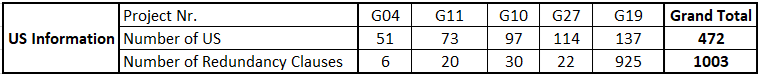
\includegraphics[scale=0.7]{Table/performance_env.png}
		\captionof{table}{Information on the backlog datasets provided for the application of the performance test}\label{tb:performance_env}
		\endgroup
	\end{figure}
	\item Tool Execution: Each part of toolchain(Rule creation, CDA tool, report creation and evaluation) was run for each backlog and the total time taken to process the entire backlog was recorded. The performance of the tool was measured by the processing time, i.e. the total time taken to process all USs in the backlog and identify redundancies.
	
	\item Repeating Tests: To ensure reliability, each test was conducted multiple times, and the average processing time was calculated.
\end{enumerate}
The test environment consisted of:
\begin{itemize}
	\item Processor: Intel(R) Core(TM) i7-8565U CPU @ 1.80GHz (8 CPUs), ~2.0GHz		
	\item Memory: 8070MB RAM
	\item Display Devices: Intel(R) UHD Graphics 620, 4163 MB(Display Memory)
	\item Hard Disk: INTEL SSDPEKNW512G8H
	\item Operating System: Windows 11 Home 64-bit (10.0, Build 22631) (22621.ni\_release.220506-1250)
	\item System Type: 64-bit operating system, x64-based processor
\end{itemize}
Table \ref{tb:performance_result} shows the result of tool's performance in seconds which were conducted on a controlled environment to ensure consistency.

	\begin{figure}[h]
	\begingroup
	\scriptsize
	\centering
	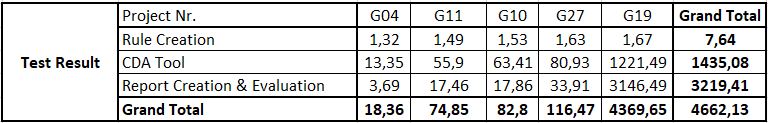
\includegraphics[scale=0.7]{Table/performance_result.png}
	\captionof{table}{Information about the result of the tool's performance test, which was measured using the processing time in seconds.}\label{tb:performance_result}
	\endgroup
\end{figure}
\paragraph{Research question 2: Conclusion}As we can see, there is a direct correlation between the number of USs in a backlog and the time our tool needs to process them. The results confirm that developers and project managers should expect a longer processing time when evaluating redundancy as the backlog grows.

However, the impact on processing time varies depending on the process in question. While rule creation using the Henshin API shows relatively consistent and lower processing times, other components such as the CDA tool and report creation processes show an exponential increase in processing time as the number of USs increases. This indicates that certain processes scale differently as the data load increases.

An important observation is that with a larger number of USs, the probability of finding redundant clauses between USs increases. This has a significant impact on redundancy detection and backlog management specially during processing of CDA tool. As the data set grows, there are more opportunities for overlaps, repetitions or similar USs that could indicate redundancy.
\subsubsection*{Threats to Validity}
When assessing the redundancy of USs through both personal assessment (ground truth) and the automated tool, several potential threats to validity must be considered. This section outlines the main threats to validity and describes how they were mitigated during the study.
\paragraph{Construct validity}It refers to the extent to which the assessment measures what it is intended to measure. The following risks were identified:
\begin{itemize}
	\item Ambiguity of criteria: If the criteria for redundancy are unclear or open to interpretation, this can lead to inconsistent scores. To avoid this, we defined clear and detailed criteria for identifying redundancy in USs.
	
	\item Subjectivity in ground truth: As ground truth is based on personal judgement, subjectivity could lead to bias. To minimise this risk, we cross-checked out evaluations with another experienced evaluator.
\end{itemize}
\paragraph{External validity}External validity refers to the generalisability of the study results to other contexts or population groups. Threats to external validity include:

\begin{itemize}
	\item specificity of USs: If the USs used in the study are too specific or context-dependent, the results may not be transferable to other projects. To mitigate this, we included 19 backlog datasets with different USs and different project types in the analysis.
	
	\item Tool Limitation: The automated tool is designed for a specific format of USs, which limits its broader applicability. Our tool depends heavily on the specific US's format (e.g. "As a \textless user\textgreater, I want to ..., so that..."), which is essential for the application of the tool. Therefore, we tested the tool in isolated contexts limited to well-formed USs and analysed its performance in a number of scenarios.
	
	Another limitation is that our tool is dependent on the specific type of annotation used for USs. In our case, these are annotations such as action, entity, their reference targets, triggers and contains. This means that the effectiveness of the tool depends on the accuracy and consistency of these annotations. If the annotations are incomplete or incorrect, the tool may not work as expected. In addition, the tool may not be compatible with other annotation schemes that do not use these specific labels.
\end{itemize}
\paragraph{Internal Validity}Internal validity is concerned with whether the observed results are attributable to the factors analysed or are influenced by other variables. Potential threats to internal validity include:
\begin{itemize}
	\item Confounding factors: External influences or unintended variables could influence the assessment of redundancy. In particular, USs annotated with Doccano are a very critical impact when evaluating full and partial redundancies between USs using tool. The more phrases are covered in the relationship(targets, contains), the better the score. Since our tool uses Doccano annotated USs as primary input without any changes, these discrepancies are unavoidable. % To avoid this, I controlled the scope of the study to ensure that all user reports came from a consistent context and that consistent evaluation methods were used.
	
	\item Limitation of tool: The automated tool may not capture all aspects of redundancy, especially semantically. This leads us to the next step, the semantic analysis of USs.
\end{itemize}
\subsection{Conclusion}\label{redundancy_conclustion}
In this study, we developed and applied a comprehensive approach that combines the Doccano tool, Henshin and the CDA tool to systematically identify and report redundancies in USs within software development projects with an evaluation.

By carefully analysing 19 different backlog datasets, our method not only separated USs into main and benefit parts for nuanced examination, but also facilitated the distinction between full and partial redundancies within these parts.

Our results reveal a crucial finding: the effectiveness of redundancy detection is significantly influenced by the quality of the USs as well as annotated USs. Well-formulated USs that do not contain unnecessary clauses (e.g. the repetition of \enquote{end product} in all USs) and a concisely annotated backlog specially in relation properties also have a major influence on the effective redundancy analysis process.

 If the main part is evaluated to be full redundant, then we have a US-pair that is functionally identical and we can merge the US-pair into one US. In the case of full redundancy in the benefit part, this means that the US-pairs belong to the same goal and objective, to which they should be categorised for better accessibility and understanding.
 
A notable trend emerged from our analysis: the benefit parts are more often fully redundant than the main parts of USs. This indicates that multiple USs often strive for different functions that contribute to a common system aspect or goal.

Recognising such redundancies not only helps to consolidate functionally identical US-pairs into single, more compact USs, but also to group US-pairs together, improving accessibility and understanding of project backlogs.

In summary, our study confirms the central role of a syntactic analysis approach in detecting and managing redundancies in project backlogs, thereby contributing to the rationalisation of software development processes.

While the quality of annotated USs plays a critical role in the success of this approach, the insights gained from this research provide valuable guidance for both current practices and future research in software project management.

However, our investigation has also shown that we can only consider USs with syntactic redundancy. If they are indeed US-pairs with the same functionality but using different words and clauses to achieve the same goal, we cannot detect this with this approach.

This finding shows that the distinction between actual redundancy and mere superficial similarity can be further refined, which leads us to analyse the USs semantically.

In the next section, we therefore present a method for analysing conflicts and dependencies between USs in semantic way.
%We also find that there are more full redundancy in the benefit part as compared to main part, as the USs with the same benefit achieve different functions for the same aspect of system.

%We have realised that some user stories are only apparently part of other USs, so we can merge them into a compact single US.
%\subsection{Evaluation}\label{redundancy_evaluation}
%In this section we will present the results of applying our approach to analyse USs in 19 by CRF tool annotated backlog datasets. 
%The purpose of this section is to assess the effectiveness of our approach in analysing redundancy between USs. This section serves several key objective:
In this section, we address two different research questions and provide a detailed explanation of the experimental design and execution for each question. We also present a detailed analysis of the results to provide answers to these research questions, highlight their implications and provide insights into the research findings.
%\begin{itemize}
%	\item Demonstrating the validity and reliability of our proposed methodology for identifying and categorising redundancies between USs.
%	\item Presenting the results of our analysis across multiple datasets, highlighting the prevalence of \enquote{Full and Partial Redundancy} for both the main and benefit parts of USs.
%	\item Gaining insights into the nature and extent of redundancies between USs and its potential impact on software development processes.
%	\item Comparing results from different data sets, identifying patterns or trends and analysing variations in redundancy levels.
%\end{itemize}
\subsubsection*{Research Questions}
The research questions addressed in this section are as follows:
\begin{enumerate}
	\item Does our tool reliably determine the level of redundancy —either partial or full— between different parts of USs (main and benefit)?
	\item How does the tool's performance scale when the number of USs in a backlog increases?
	\end{enumerate}
\subsubsection*{Methodology}
To address the first questions "Does our tool reliably determine the level of redundancy—either partial or full—between different parts of USs (main and benefit)?", we recap the methodology employed to analyse redundancy between USs. We utilized a systematic approach that involved several key steps:
\begin{itemize}
	
	\item Data Collection: For a comprehensive assessment, we applied our approach to 19 backlog datasets presented by Mosser et al.\footnote{https://github.com/ace-design/nlp-stories}. They applied the Doccano approach to these publicly available requirements datasets\cite{requirementsdatasets}.
	
	It is also worth noting that some backlog datasets (g02, g13, g17, g27) did not follow the expected sentence structure, which is why we did not include them in the evaluation results to avoid unexpected behaviour. Table \ref{tb:backlogs} shows the project number of each dataset and the count of USs.
	%	- You have to describe all that in your work, how do you define Main Partial/Full and Benefit Partial/Full, so how do you decide that. And generating this JSON_Report and filling this table is all interesting implementation information.
	
	%When evaluating, I use tools on a large scale and I go through all the cases and look at what comes out of the use case as a meaningful result. As an evaluation, I will enter all the datasets we have as input and then what comes out will be 
	\begingroup
	\centering
	\scriptsize
	\renewcommand{\arraystretch}{1.5} 
	%\keepXColumns
	\begin{tabularx}{\linewidth}{l|XXXXXXXXXXXXXXXXXXX|X}
		Item&	1&	2&	3&	4&	5&	6&	7&	8&	9&	10&	11&	12&	13&	14&	15&	16&	17&	18&	19&	\\
		\hline
		%Project Name&loudoun&recycling&openspending&frictionless&scrumalliance	&nsf&camperplus&datahub&mis&neurohub&alfred&badcamp&rdadmp&archivesspace	&unibath&duraspace&racdam&culrepo&zooniverse&\\
		Project Nr.&	g03	&g04	&g05	&g08	&g10	&g11	&g12	&g14	&g16	&g18	&g19	&g21	&g22	&g23	&g24	&g25	&g26	&g27	&g28	&Total USs\\
		\hline
		Total USs&	57&	51	&53	&66	&97	&73	&54	&67	&66	&102	&137	&69	&83	&56	&53	&100	&100	&114	&60	&1458 \\
		\caption{Project number and count of USs contained in each backlog dataset}\label{tb:backlogs}
	\end{tabularx}	
	\endgroup
	
	%\item Preprocessing: Using the generated JSON report file for each dataset, we create a VBA script called \textit{extractFromJSONFiles}\footnote{https://github.com/amirrabieyannejad/USs\_Annotation/tree/main/Skript/extractFromJSONFiles} to iterate through all the JSON report files and extract the information such as \enquote{US-pair}, \enquote{US-text}, \enquote{total redundancy clauses}, \enquote{main redundancy clauses}, \enquote{benefit redundancy clauses} and \enquote{project number} and collect them all in an Excel file to perform further analyses.
	
	\item Identification of main and benefit parts: Each US was divided into its main part, which is the core functionality, and its benefit part, which describes the value to the persona.
	
	\item Detection of overlapping clauses: Recognition of overlapping clauses between a US-pair in a specific part of the USs.
	
	\item Redundancy analysis in main and benefit parts: Based on the redundant clauses identified, an automatic redundancy analysis was performed for the main and benefit parts of the US-pair based on certain criteria indicating the level of redundancy (partial or full) in the main and benefit parts.
		
	%\item Preprocessing: \item preprocessing: We transform each data set into graph transformation rules, apply CDA and generate a textual report in which each redundancy clause between US-pairs is marked with a hash symbol. Additionally,  the number of founded redundancies in the main and benefit sections is also determined.
\end{itemize}
\subsubsection*{Ground Truth Evaluation of US Redundancy}
Answering the first research question requires our automated system to have a reference point against which its accuracy can be measured. This reference point or "ground truth" is derived from a personal assessment and serves as a benchmark for the tool's performance.

In contrast to the tool evaluation, we did not evaluate based on labels (e.g., action, entity, persona, targets, etc.) in the personal evaluation. This means that when evaluating ground truth, we evaluate partial and full redundancy based on the phrases occurring in a given part as a one-to-one comparison.

The ground truth is the final assessment against which automated results are compared. It is derived from the personal judgement of a subject matter expert (in this case myself) using a combination of expertise, experience and specific evaluation criteria. The personal assessment is targeted at providing a reliable and accurate reference for redundancy between USs.\\\\
	The following criteria were taken into account in the personal assessment:
	\begin{itemize}
		\item A US-pair is evaluated as fully redundant in the main part, if all phrases occurred in the main parts of both USs fully overlap with one-to-one comparison. For example, the following US-pair is assessed as fully redundant:\\
		user\_story\_01: "\#g14\# as a \#publisher\#, i want to \#publish\# a \#dataset\#, so that i can view just the dataset with a few people."
		
		user\_story\_02: "\#g14\# as a \#publisher\#, i want to \#publish\# a \#dataset\#, so that i can share the dataset publicly with everyone."
		
		\item A US-pair is considered fully redundant in the main part, if all phrases in the main part of at least one US completely overlap. For instance:\\
		user\_story\_22: "\#g14\# as a \#consumer\#, i want to \#view\# a \#data package\# online, so that i can \#get\# a \#sense\# of whether this is the dataset i want."
		
		user\_story\_24: "\#g14\# as a \#consumer\#, i want to \#view\# the \#data package\#, so that that i can \#get\# a \#sense\# of whether i want this dataset or not."
		
		\item A US-pair is categorised as partially redundant in the main part if some phrases remain distinctive between the USs. For Instance:\\
		user\_story\_09: "\#g04\# as a \#user\#, i want to be able to \#view\# a \#map display\# of the public recycling bins around my \#area\#."
		
		user\_story\_10: "\#g04\# as a \#user\#, i want to be able to \#view\# a \#map display\# of the special waste drop off sites around my \#area\#."
		
		\item The criteria mentioned were also applied to the benefit part.
	\end{itemize}
Table \ref{tb:ground_truth} shows the aggregation of full and partial redundancies in the main and benefit parts as ground truth.
\begin{figure}[h]
	\begingroup
	\scriptsize
	\centering
	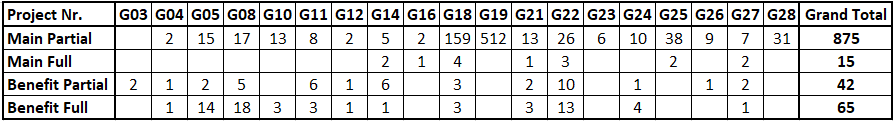
\includegraphics[scale=0.6]{Table/ground_truth.png}
	\captionof{table}{Detail about full and partial redundancies related to main or benefit parts as ground truth}\label{tb:ground_truth}
	
	\endgroup
\end{figure}
As we can see, the main parts of the US-pairs have less full redundancy (15 cases), which means that there are 15 cases where the main part of the US-pairs is exactly the same. This level of redundancy indicates common functionality of the US-pairs, which is a sign of overlapping features. 

A much higher occurrence of partial redundancy in the main parts(875 cases) indicates that there are common elements between the US-pairs, but still enough differences to avoid a complete match. 

Fewer instances of partial redundancy in the benefit parts (42 cases) indicate that the USs diverge in their benefit clauses, they are more tailored to specific project outcomes. 

The higher count of full redundancies (42 cases) compared to partial redundancies in the benefit parts is interesting, as it indicates that the expected objectives of certain features are often repeated in the USs. This suggests that the project is aiming for a set of common goals regardless of the specific functionality.
\subsubsection*{Evaluation of US Redundancy using Tool}
The automated tool is designed to identify redundancy among USs based on predefined criteria. It operates by analysing the text and structure of USs to detect similarities that could indicate redundancy.

In contrast to ground truth, which is based on one-to-one comparison of phrases in specific parts of USs, tool evaluation relies heavily on specified labelling (targets, triggers, contains) using the Doccano tool.

The following criteria are defined for the evaluation of US-pairs:
\begin{itemize}
	\item Full redundancy: 	A pair of US is considered to have "full redundancy" in the main or benefit part when every labelled clause in that part—comprising triggers (in the main part), targets, and contains—is syntactically identical.
	
	\item Partial redundancy: When only some labelled clauses, such as targets, have significant overlap but are not completely identical. This means that while certain labelled clauses, such as targets, may match between USs, other labelled clauses, such as triggers or contains, may differ, meaning that the USs are not fully redundant. This scenario suggests that while USs have significant similarities, they still contain unique aspects.
\end{itemize}
Table \ref{tb:tool} shows the aggregation of the full and partial redundancies in the main and benefit parts assessed by the tool. It is also worth noting that the numbers highlighted in red show the variation in the ground truth evaluation.
\begin{figure}[h]
	\begingroup
	\scriptsize
	\centering
	\includegraphics[scale=0.6]{Table/tool.png}
	\captionof{table}{Aggregation of the count of full and partial redundancies in relation to the main or benefit parts assessed by the tool}\label{tb:tool}
	\endgroup
\end{figure}
\paragraph{Assessment of Result: High-Level Overview}Based on the datasets provided, it was found that 1,851 redundancy clauses were identified across all projects, with the highest count found in the backlog G19 dataset (925 clauses), indicating a significant presence of redundancy in the USs of this project. 

Table \ref{tb:redundancy_clauses} shows the total number of redundancy clauses found in each dataset.
\begin{figure}[h]
	\begingroup
	\scriptsize
	\centering
	\includegraphics[scale=0.55]{Table/redundancy_clauses.png}
	\captionof{table}{Detail about number of redundancy clauses occurred in main and benefit parts}\label{tb:redundancy_clauses}
	
	\endgroup
\end{figure}
\paragraph{Assessment of Result: Aggregated Analysis}We also look for an aggregate for the count of redundant clauses in both the main and the benefit parts of the USs. 

In the main parts, the large count of full redundancies, especially where two clauses are present (6 clauses), indicates a high degree of similarity in the functionalities described.

In the benefit part of the USs, there is a considerable count of cases where full redundancy prevails, especially where two clauses are inserted (24 clauses). The large count of full redundancies with two clauses indicates that benefits are often described in a standardised way in the different USs.

Figure \ref{fig:aggregation} illustrates the aggregation of the count of redundancy clauses that occur in USs.

\begin{figure}[h]
	\centering
	\includegraphics[scale=0.5]{aggregation_benefit}
	\includegraphics[scale=0.5]{aggregation_main}
	\caption{The aggregation between the count of redundancy clauses occurred in USs}\label{fig:aggregation}
\end{figure}
\paragraph{Assessment of Result: Detailed Insights}In the dataset of Backlog G19, the clause \enquote{have alfred} was repeated in all USs, indicating that \enquote{alfred} is the end product and not a specific functionality. This suggests that the quality of the USs should be considered, so that they do not contain generic information that results in a lot of redundant information(false positives) being provided.

In the main parts of the USs, 1,663 clauses were redundant("Main Part Redundancy Clauses" in Table \ref{tb:redundancy_clauses}), while only 188 redundancy clauses were found in the benefit parts("Benefit Part Redundancy Clauses" in Table \ref{tb:redundancy_clauses}). This means that some USs are not often written in a standardised format for the description of core functions, resulting in a higher count of redundant clauses in the main part.
\begin{example}
	In the dataset of backlog G18 (274 clauses out of 283 in the main parts), for example, this is due to the clauses \enquote{have ability} in the main part, which are unnecessarily repeated in most USs:\\
	\textit{user\_story\_92:} \#g18\# as a \#researcher\# I want to have \#the \#ability\# to search files by file type and format.\\
	\textit{user\_story\_80:} \#g18\# as a \#researcher\# I want to have \#the \#ability\# to attach standard metadata for behavioural observations (and video) so that my data can be searched and understood later.\\
	Actually, the clause \enquote{have ability} in USs should be deleted and no redundancy should be possible at all:\\
	\textit{user\_story\_92:} \#g18\# as a researcher I want to search for files by file type and format.\\
	\textit{user\_story\_80:} \#As a researcher, I want to attach standard metadata for behavioural observations (and videos), so that my data can be searched and understood later.
\end{example}

There are also USs with the same functionality, but one provides more details about the functionality. In other words, one US is contained within another, and we refer to them as full
redundant US-pairs, as deleting the US with less detail has no negative impact on the system. Sometimes it is necessary to merge these two USs to obtain a single detailed US.
\begin{example}
	In the dadaset of backlog G18, for example, we have two US-pairs that are marked as full redundancy between user\_story\_12 and user\_story\_11 as well as user\_story\_13 and user\_story\_11:\\
	\textit{user\_story\_12}: \enquote{\#g18\# as a \#researcher\#, I want to \#upload\# \#files\# prior to having them \#attached\# to a \#log book page\# using the web interface.}\\
	\textit{user\_story\_11:} \enquote{\#g18\# as a \#researcher\#, I want to \#upload\# \#files\# prior to having them \#attached\# to a \#log book page\#.}\\
	\textit{user\_story\_13:} \enquote{\#g18\# as a \#researcher\#, I want to \#upload\# \#files\# prior to having them \#attached\# to a \#log book page\# using a mapped network drive.}\\
	
	As we can see, the user\_story\_11 is an incomplete version of two other USs, and deleting it has no negative impact in the system, due to the fact that its goal is achieved and fulfilled by two other USs.
\end{example}
\paragraph{Research question 1: Conclusion}
After comparing the Ground Truth result with the result provided by our tool, the following realisation was made:
\begin{itemize}
	\item Main Part Partial: A -5.6\% (negative) percentage suggests that the Framework has fewer "Main Part Partial" counts than the Ground Truth.
	In this case, the Framework has about 5.6\% fewer "Main Part Partial" counts than expected.
	
	\item Main Part Full: A high positive percentage of 326.67\% indicates that the Framework has a significantly higher count of Main Part Full compared to Ground Truth.
	At 326.67\%, the framework has more than three times as many main part full compared to the ground truth.
	In our investigation, we found that some phrases are not included as relationship (contains or targets) in the USs annotated with the Doccano tool. Therefore, our tool categorised some USs as fully redundant when in reality they were only partially redundant.
	
	\item Count of Benefit Partial: -26.19\% a negative percentage here indicates that the Framework has fewer "Benefit Partial" counts compared to the Ground Truth.
	With -26.19\%, the Framework has approximately one-quarter fewer "Benefit Partial" counts.
	
	\item Count of Benefit Full: 16.92\% a positive percentage indicates that the Framework has more "Benefit Full" counts compared to the Ground Truth.
	With 16.92\%, the Framework has almost 17\% more "Benefit Full" counts than the Ground Truth.
\end{itemize}
It is also notable that if we add founded partial and full redundancies in main or benefit parts, we both amount are identical(main part: 890 cases , benefit part: 107).

This consistency indicates that the automated tool's results align with the ground truth, suggesting that the tool is reliable in detecting redundancy. It demonstrates that the tool's performance closely matches the personal assessment, reinforcing confidence in its accuracy and validity.
\subsubsection*{Performance Evaluation}
To answer the second research question "How does the tool's performance scale as the count of USs in a backlog increases?", we conducted a series of tests to measure the time it takes the tool to process different counts of USs. This section describes the testing methodology, the results obtained and the impact on the scalability of the tool.
\paragraph{Test Methodology}To evaluate the tool's performance, we conducted a set of experiments in which the tool processed different numbers of USs in a backlog. The tests involved the following steps:
\begin{enumerate}
	\item Backlog Setup: We used backlogs with varying numbers of USs around—50, 70, 90, 120 and 140—to simulate different workload sizes. Each backlog contained USs with varying content, redundancy elements, and complexity to represent a realistic range of cases. Table \ref{tb:performance_env} shows information on the backlog data records provided for the performance test application.
	\begin{figure}[h]
		\begingroup
		\scriptsize
		\centering
		\includegraphics[scale=0.7]{Table/performance_env.png}
		\captionof{table}{Information on the backlog datasets provided for the application of the performance test}\label{tb:performance_env}
		\endgroup
	\end{figure}
	\item Tool Execution: Each part of toolchain(Rule creation, CDA tool, report creation and evaluation) was run for each backlog and the total time taken to process the entire backlog was recorded. The performance of the tool was measured by the processing time, i.e. the total time taken to process all USs in the backlog and identify redundancies.
	
	\item Repeating Tests: To ensure reliability, each test was conducted multiple times, and the average processing time was calculated.
\end{enumerate}
The test environment consisted of:
\begin{itemize}
	\item Processor: Intel(R) Core(TM) i7-8565U CPU @ 1.80GHz (8 CPUs), ~2.0GHz		
	\item Memory: 8070MB RAM
	\item Display Devices: Intel(R) UHD Graphics 620, 4163 MB(Display Memory)
	\item Hard Disk: INTEL SSDPEKNW512G8H
	\item Operating System: Windows 11 Home 64-bit (10.0, Build 22631) (22621.ni\_release.220506-1250)
	\item System Type: 64-bit operating system, x64-based processor
\end{itemize}
Table \ref{tb:performance_result} shows the result of tool's performance in seconds which were conducted on a controlled environment to ensure consistency.

	\begin{figure}[h]
	\begingroup
	\scriptsize
	\centering
	\includegraphics[scale=0.7]{Table/performance_result.png}
	\captionof{table}{Information about the result of the tool's performance test, which was measured using the processing time in seconds.}\label{tb:performance_result}
	\endgroup
\end{figure}
\paragraph{Research question 2: Conclusion}As we can see, there is a direct correlation between the number of USs in a backlog and the time our tool needs to process them. The results confirm that developers and project managers should expect a longer processing time when evaluating redundancy as the backlog grows.

However, the impact on processing time varies depending on the process in question. While rule creation using the Henshin API shows relatively consistent and lower processing times, other components such as the CDA tool and report creation processes show an exponential increase in processing time as the number of USs increases. This indicates that certain processes scale differently as the data load increases.

An important observation is that with a larger number of USs, the probability of finding redundant clauses between USs increases. This has a significant impact on redundancy detection and backlog management specially during processing of CDA tool. As the data set grows, there are more opportunities for overlaps, repetitions or similar USs that could indicate redundancy.
\subsubsection*{Threats to Validity}
When assessing the redundancy of USs through both personal assessment (ground truth) and the automated tool, several potential threats to validity must be considered. This section outlines the main threats to validity and describes how they were mitigated during the study.
\paragraph{Construct validity}It refers to the extent to which the assessment measures what it is intended to measure. The following risks were identified:
\begin{itemize}
	\item Ambiguity of criteria: If the criteria for redundancy are unclear or open to interpretation, this can lead to inconsistent scores. To avoid this, we defined clear and detailed criteria for identifying redundancy in USs.
	
	\item Subjectivity in ground truth: As ground truth is based on personal judgement, subjectivity could lead to bias. To minimise this risk, we cross-checked out evaluations with another experienced evaluator.
\end{itemize}
\paragraph{External validity}External validity refers to the generalisability of the study results to other contexts or population groups. Threats to external validity include:

\begin{itemize}
	\item specificity of USs: If the USs used in the study are too specific or context-dependent, the results may not be transferable to other projects. To mitigate this, we included 19 backlog datasets with different USs and different project types in the analysis.
	
	\item Tool Limitation: The automated tool is designed for a specific format of USs, which limits its broader applicability. Our tool depends heavily on the specific US's format (e.g. "As a \textless user\textgreater, I want to ..., so that..."), which is essential for the application of the tool. Therefore, we tested the tool in isolated contexts limited to well-formed USs and analysed its performance in a number of scenarios.
	
	Another limitation is that our tool is dependent on the specific type of annotation used for USs. In our case, these are annotations such as action, entity, their reference targets, triggers and contains. This means that the effectiveness of the tool depends on the accuracy and consistency of these annotations. If the annotations are incomplete or incorrect, the tool may not work as expected. In addition, the tool may not be compatible with other annotation schemes that do not use these specific labels.
\end{itemize}
\paragraph{Internal Validity}Internal validity is concerned with whether the observed results are attributable to the factors analysed or are influenced by other variables. Potential threats to internal validity include:
\begin{itemize}
	\item Confounding factors: External influences or unintended variables could influence the assessment of redundancy. In particular, USs annotated with Doccano are a very critical impact when evaluating full and partial redundancies between USs using tool. The more phrases are covered in the relationship(targets, contains), the better the score. Since our tool uses Doccano annotated USs as primary input without any changes, these discrepancies are unavoidable. % To avoid this, I controlled the scope of the study to ensure that all user reports came from a consistent context and that consistent evaluation methods were used.
	
	\item Limitation of tool: The automated tool may not capture all aspects of redundancy, especially semantically. This leads us to the next step, the semantic analysis of USs.
\end{itemize}
\subsection{Conclusion}\label{redundancy_conclustion}
In this study, we developed and applied a comprehensive approach that combines the Doccano tool, Henshin and the CDA tool to systematically identify and report redundancies in USs within software development projects with an evaluation.

By carefully analysing 19 different backlog datasets, our method not only separated USs into main and benefit parts for nuanced examination, but also facilitated the distinction between full and partial redundancies within these parts.

Our results reveal a crucial finding: the effectiveness of redundancy detection is significantly influenced by the quality of the USs as well as annotated USs. Well-formulated USs that do not contain unnecessary clauses (e.g. the repetition of \enquote{end product} in all USs) and a concisely annotated backlog specially in relation properties also have a major influence on the effective redundancy analysis process.

 If the main part is evaluated to be full redundant, then we have a US-pair that is functionally identical and we can merge the US-pair into one US. In the case of full redundancy in the benefit part, this means that the US-pairs belong to the same goal and objective, to which they should be categorised for better accessibility and understanding.
 
A notable trend emerged from our analysis: the benefit parts are more often fully redundant than the main parts of USs. This indicates that multiple USs often strive for different functions that contribute to a common system aspect or goal.

Recognising such redundancies not only helps to consolidate functionally identical US-pairs into single, more compact USs, but also to group US-pairs together, improving accessibility and understanding of project backlogs.

In summary, our study confirms the central role of a syntactic analysis approach in detecting and managing redundancies in project backlogs, thereby contributing to the rationalisation of software development processes.

While the quality of annotated USs plays a critical role in the success of this approach, the insights gained from this research provide valuable guidance for both current practices and future research in software project management.

However, our investigation has also shown that we can only consider USs with syntactic redundancy. If they are indeed US-pairs with the same functionality but using different words and clauses to achieve the same goal, we cannot detect this with this approach.

This finding shows that the distinction between actual redundancy and mere superficial similarity can be further refined, which leads us to analyse the USs semantically.

In the next section, we therefore present a method for analysing conflicts and dependencies between USs in semantic way.
%We also find that there are more full redundancy in the benefit part as compared to main part, as the USs with the same benefit achieve different functions for the same aspect of system.

%We have realised that some user stories are only apparently part of other USs, so we can merge them into a compact single US.
%\input{Section/Redundancy_Evaluation}


